\section{Benchmarking}
\label{sec:res_bench}
This section presents the result from the IOZone benchmarking tests run on each filesystem. The benchmarking was completed successfully for all file sizes for \gls{FFFS} and \gls{APFS}. For the biggest file size, \SI{262144}{\kilo\byte}, \gls{GCSF} crashed multiple times, but it succeeded for the other file sizes. \gls{FFS} crashed multiple times for the \SI{262144}{\kilo\byte} file size when the \gls{UBC} was disabled but completed successfully for this file size when the \gls{UBC} was enabled. It was found during debugging that \gls{FFS} could not close a file of \SI{200}{\mega\byte} without \gls{FFS} crashing, seemingly due to a \gls{FUSE} error. Unfortunately, the reason behind these crashes was not found. Therefore, the results for the biggest file size were omitted from the tests of \gls{FFS} with the \gls{UBC} disabled, and for \gls{GCSF} for both states of the \gls{UBC}. Each of the six filesystems was benchmarked 20 times with the \gls{UBC} enabled and 20 times with the \gls{UBC} disabled. Nine file sizes were used (eight file sizes for \gls{FFS} with the \gls{UBC} disabled and for \gls{GCSF}) and up to 13 buffer sizes per file size. Each test per filesystem produced a table with nine rows (eight rows for \gls{FFS} with the \gls{UBC} disabled and \gls{GCSF}) and 13 columns, where each cell is the average performance of the 20 tests with the specific file size and buffer size on the filesystem. The tables for \gls{FFFS} and \gls{APFS} with both states of the \gls{UBC} and the table for \gls{FFS} with the \gls{UBC} enabled have 107 cells, while the table for \gls{FFS} with the \gls{UBC} disabled and the tables for \gls{GCSF} with both states of the \gls{UBC} have 94 cells. See Appendix~\ref{app:bench_data} starting on page \pageref{app:bench_data} for the tables.

The bandwidth used by the computer during the benchmarks was measured by Wireshark by capturing the number of bytes sent per ten-second interval. \Cref{tbl:sniff-data} presents the bandwidth in kilobits per second as recorded by Wireshark during the benchmarking of \gls{FFS} and \gls{GCSF}, with the \gls{UBC} enabled and disabled. Each data point is the incoming and outgoing bandwidth per ten-second window. For instance, it can be seen that the minimum bandwidth of \gls{GCSF} is \SI[per-mode = symbol]{0.00}{\kilo\byte\per\second}, meaning that no data was sent or received over the internet on the network interface of the computer during at least one ten second window. It can be observed that the maximum bandwidth of either filesystem does not exceed \SI[per-mode = symbol]{26}{\mega\bit\per\second}. \SI[per-mode = symbol]{26}{\mega\bit\per\second} is higher than the upload bandwidth of the internet subscription (\SI[per-mode = symbol]{20}{\mega\bit\per\second}) but significantly lower than the download bandwidth of the subscription (\SI[per-mode = symbol]{100}{\mega\bit\per\second}).

\begin{table}[!ht]
	\begin{center}
	\caption{Network bandwidth during the benchmarks of the cloud-based filesystems}
	
	\resizebox{\textwidth}{!}{
		\begin{tabular}{| r | r | r | r | r | }
			\hline
			{} & \multicolumn{4}{c |}{Bandwidth (kbit/s)} \\
		 	\multicolumn{1}{| c |}{\textbf{Filesystem}} & \multicolumn{1}{c |}{Minimum} & \multicolumn{1}{c |}{Average} & \multicolumn{1}{c |}{Median} & \multicolumn{1}{c |}{Maximum} \\
		 	\hline
		 	\hline
FFS, UBC Enabled & 0.28 & 636.26 & 241.02 & 12214.97\\
FFS, UBC Disabled & 0.11 & 310.61 & 185.28 & 17720.17\\
GCSF, UBC Enabled & 0.00 & 621.34 & 496.20 & 15781.85\\
GCSF, UBC Disabled & 0.00 & 512.95 & 403.32 & 25538.91\\


			\hline

		\end{tabular}
		}
		\label{tbl:sniff-data}
	\end{center}
\end{table}


Combining all the data points from one benchmark test for a filesystem over all 20 iterations, we get the overall performance of the test on the filesystem. With this data, we can use a box plot to present the values in the table, and by combining the results from all filesystems for a specific test, we can compare their box plots in one figure. Figure~\ref{fig:res_box_read} presents a box plot of the benchmarking results of the filesystems for the Read test. It can be observed that the read operation performance of \gls{FFS} and \gls{GCSF} with the \gls{UBC} enabled are in general worse than the performance for \gls{FFFS} and \gls{APFS} with the \gls{UBC} enabled. With the \gls{UBC} disabled, the median performance of \gls{GCSF} is higher than the median value of \gls{APFS}, and the median performance of \gls{FFS} and \gls{FFFS} are significantly worse. \gls{APFS} has a wide spread of values when the \gls{UBC} is disabled. All filesystems perform significantly better with the \gls{UBC} enabled. Note that the orders of the presentation of the boxplots is consistent across all of the \Cref{fig:res_box_read,fig:res_box_write,fig:res_box_reread,fig:res_box_rewrite,fig:res_box_rndread,fig:res_box_rndwrite}.

\begin{sidewaysfigure}[!ht]
	\label{fig:res_box_read}
	\begin{center}
		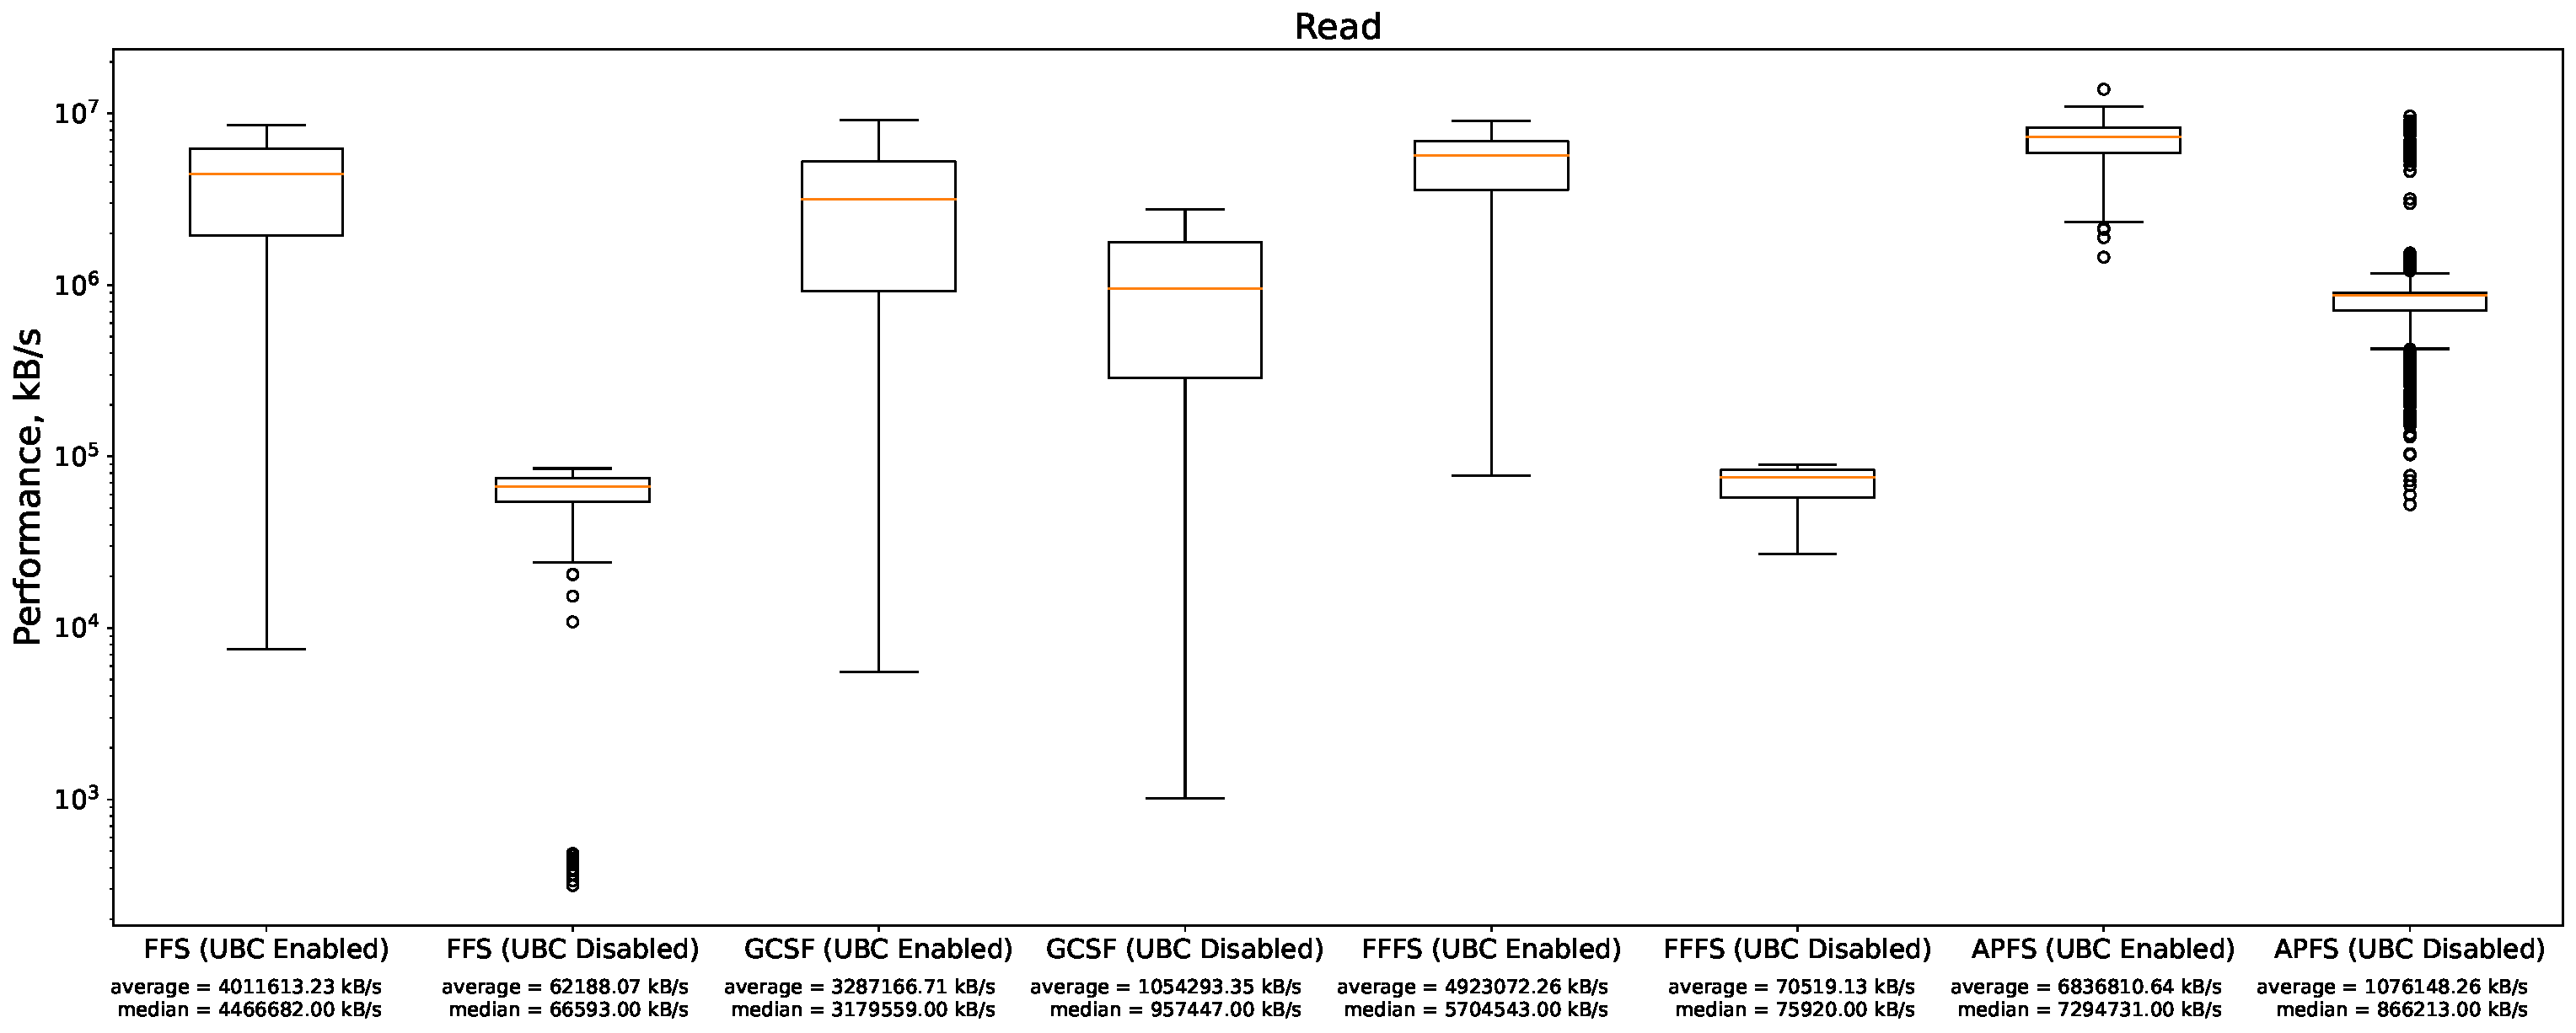
\includegraphics[width=1.0\textwidth]{figures.nosync/benchmarking/Read-boxplot.pdf}
	\end{center}
	\caption[Box plot of the IOZone output for the Read test]{Box plot of the IOZone output for the Read test on the different filesystems}
\end{sidewaysfigure}

\FloatBarrier

Figure~\ref{fig:res_box_write} presents a box plot of the benchmarking results of the filesystems of the Write test. \gls{APFS} has the best write performance of the four filesystems, both when the \gls{UBC} is enabled and when it is disabled. \gls{FFFS} performs better than the \mbox{cloud-based} filesystems for both states of the \gls{UBC}. \gls{FFFS} and \gls{GCSF} have similar performance when the \gls{UBC} is enabled and when it is disabled, while \gls{FFS} and \gls{APFS} perform significantly better with the \gls{UBC} enabled.

\begin{sidewaysfigure}[!ht]
	\label{fig:res_box_write}
	\begin{center}
		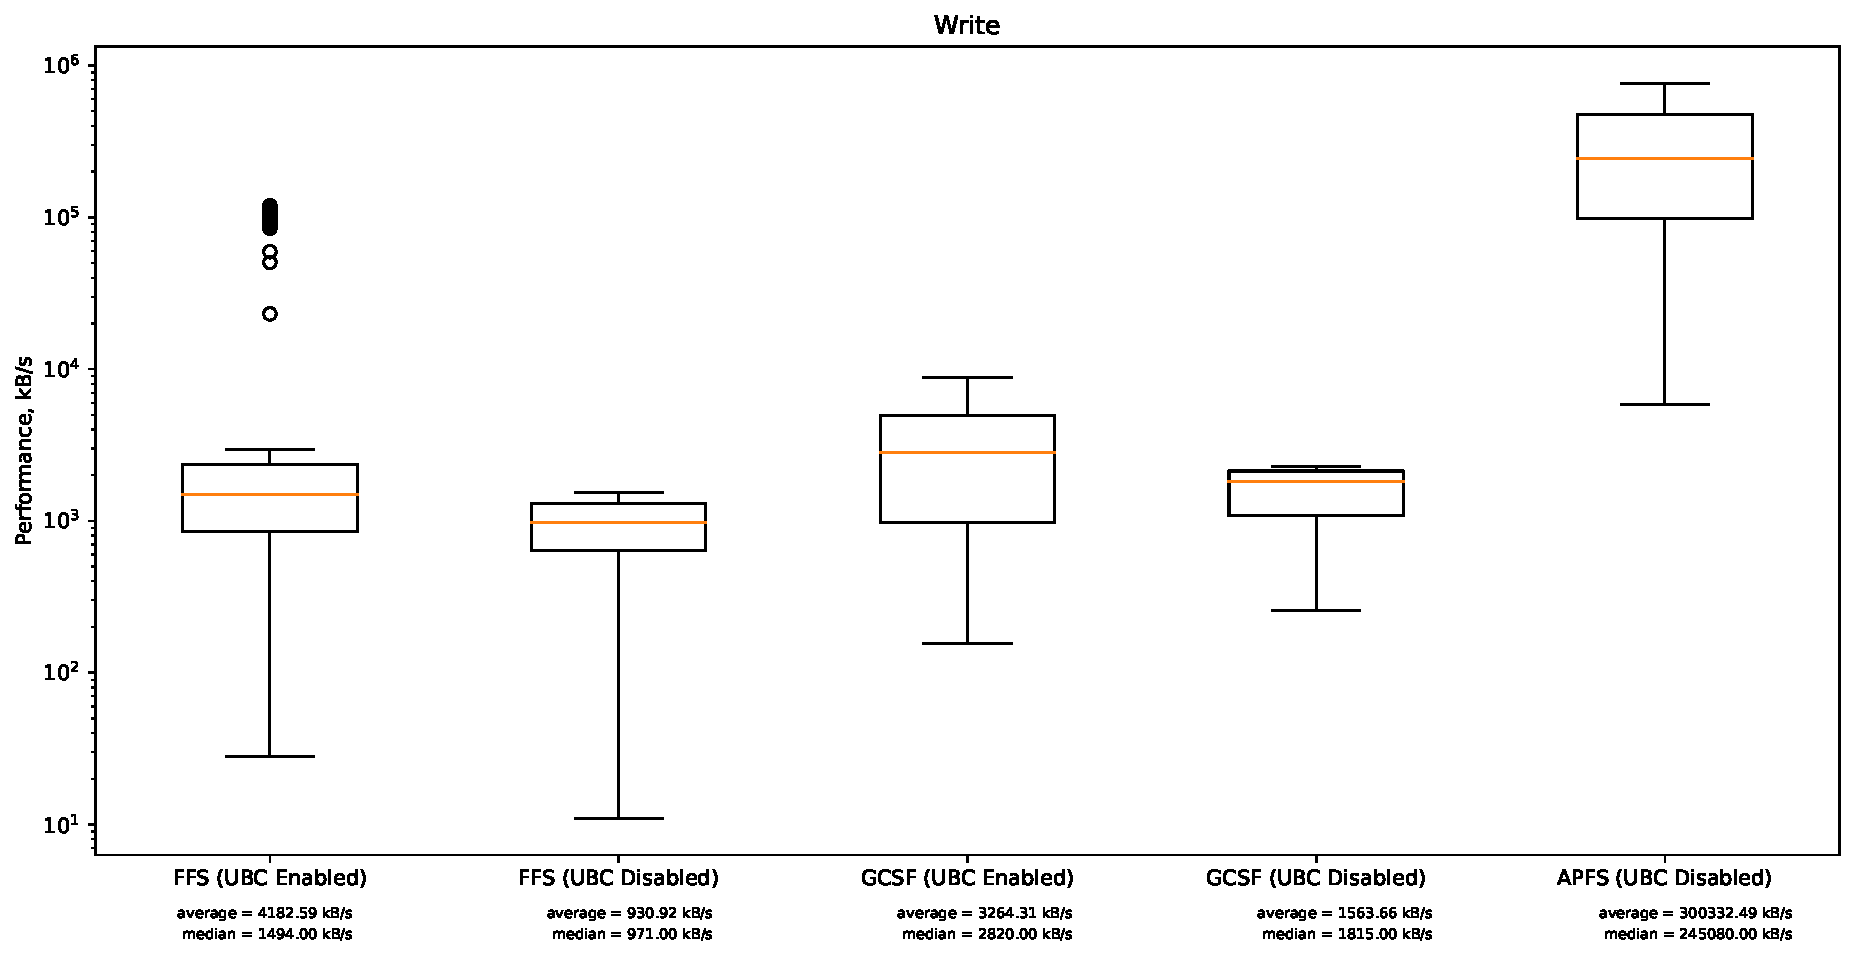
\includegraphics[width=1.0\textwidth]{figures.nosync/benchmarking/Write-boxplot.pdf}
	\end{center}
	\caption[Box plot of the IOZone output for the Write test]{Box plot of the IOZone output for the Write test on the different filesystems}
\end{sidewaysfigure}

\FloatBarrier

Figure~\ref{fig:res_box_reread} presents the result of the \mbox{Re-Read} test for the filesystems. \gls{FFS}, \gls{GCSF}, and \gls{FFFS} perform significantly better with the \gls{UBC} enabled compared to when it is disabled. \gls{APFS} also performs better with the \gls{UBC} enabled, but the performance difference compared to when the \gls{UBC} is disabled is not as large as for the other filesystems. When the \gls{UBC} is disabled, \gls{GCSF} performs better than \gls{FFS} and \gls{FFFS}. Although, when the \gls{UBC} is disabled, \gls{GCSF} has a greater spread of values with its worst performance being lower than the worst performance of \gls{FFS} and \gls{FFFS} when the \gls{UBC} is disabled.

\begin{sidewaysfigure}[!ht]
	\label{fig:res_box_reread}
	\begin{center}
		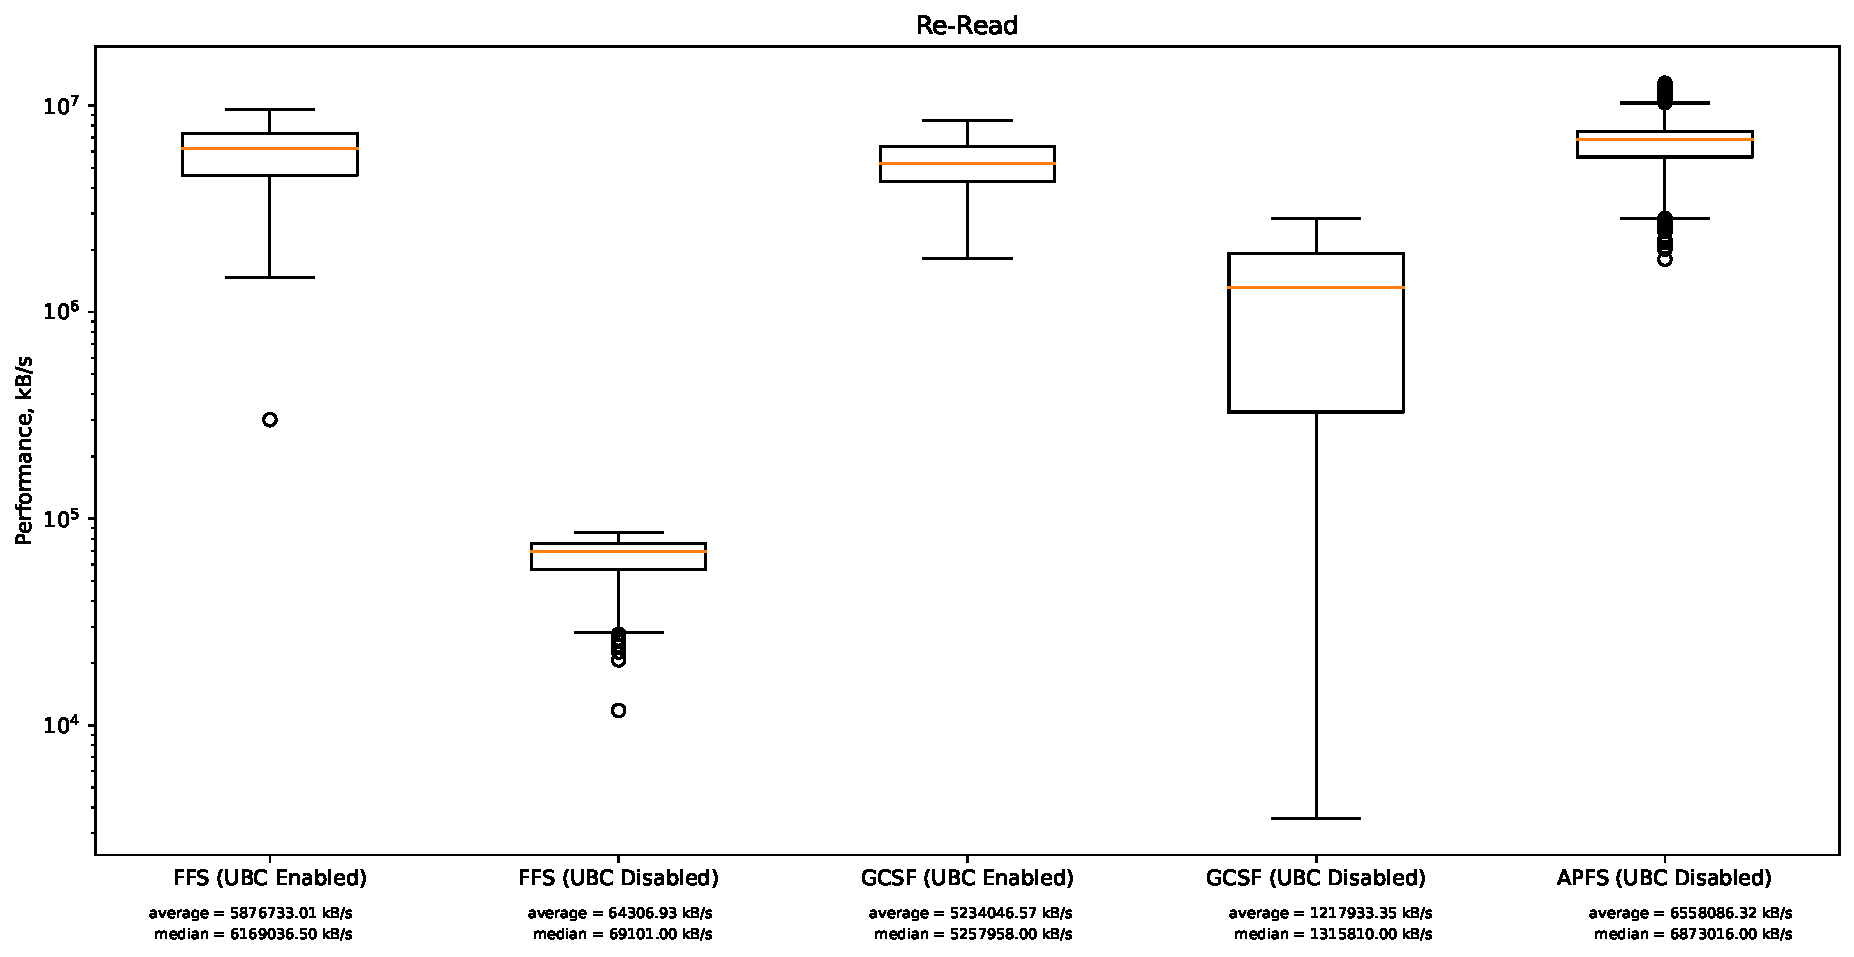
\includegraphics[width=1.0\textwidth]{figures.nosync/benchmarking/Re-Read-boxplot.pdf}
	\end{center}
	\caption[Box plot of the IOZone output for the Re-Read test]{Box plot of the IOZone output for the Re-Read test on the different filesystems}
\end{sidewaysfigure}

\FloatBarrier

Figure~\ref{fig:res_box_rewrite} presents a box plot for the \mbox{Re-Write} test for the filesystems. Similar to the Write test results presented in Figure~\ref{fig:res_box_write}, \gls{APFS} has the best performance of the filesystems, both when the \gls{UBC} is enabled and when it is disabled. \gls{FFFS} performs better than the \mbox{cloud-based} filesystems for both states of the \gls{UBC}. \gls{FFS} has slightly better average performance compared to \gls{GCSF} when the \gls{UBC} is enabled, but worse median performance. \gls{GCSF} has better average and median performance than \gls{FFS} when the \gls{UBC} is disabled.

\begin{sidewaysfigure}[!ht]
	\label{fig:res_box_rewrite}
	\begin{center}
		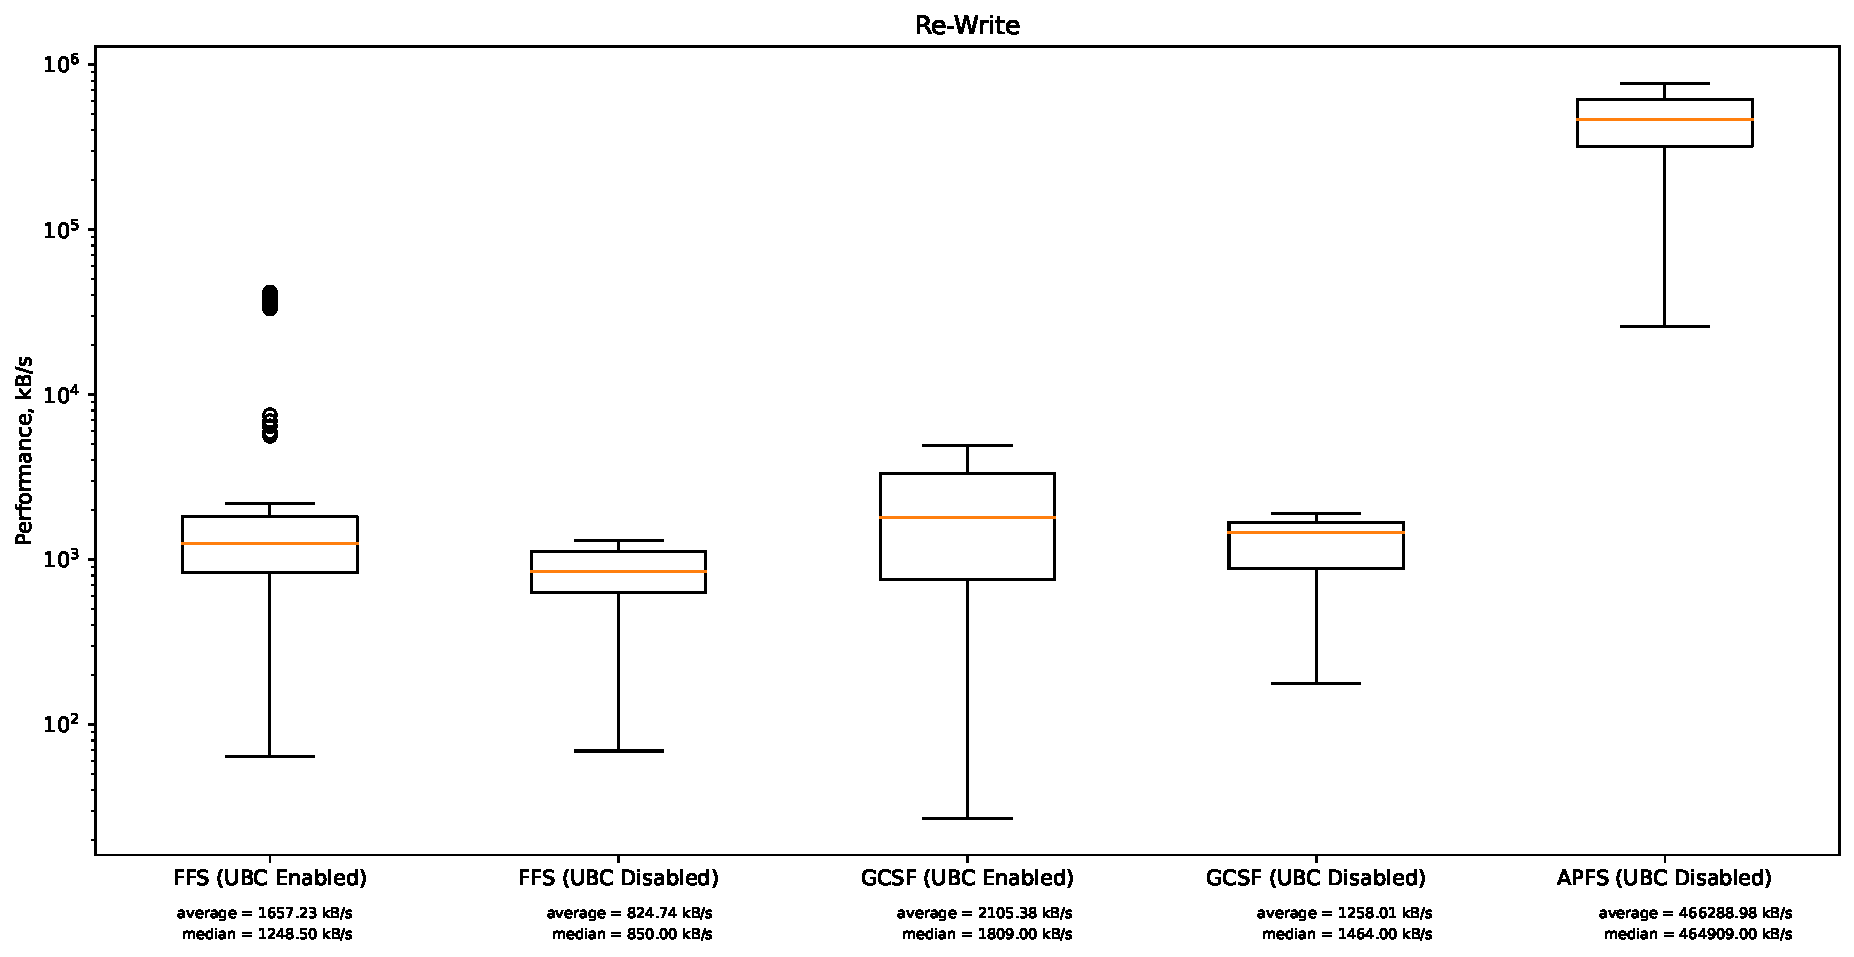
\includegraphics[width=1.0\textwidth]{figures.nosync/benchmarking/Re-Write-boxplot.pdf}
	\end{center}
	\caption[Box plot of the IOZone output for the Re-Write test]{Box plot of the IOZone output for the Re-Write test on the different filesystems}
\end{sidewaysfigure}

\FloatBarrier

Figure~\ref{fig:res_box_rndread} presents a box plot for the Random read test for the different filesystems. The results are similar to the results for the \mbox{Re-Read} test presented in Figure~\ref{fig:res_box_reread}.

\begin{sidewaysfigure}[!ht]
	\label{fig:res_box_rndread}
	\begin{center}
		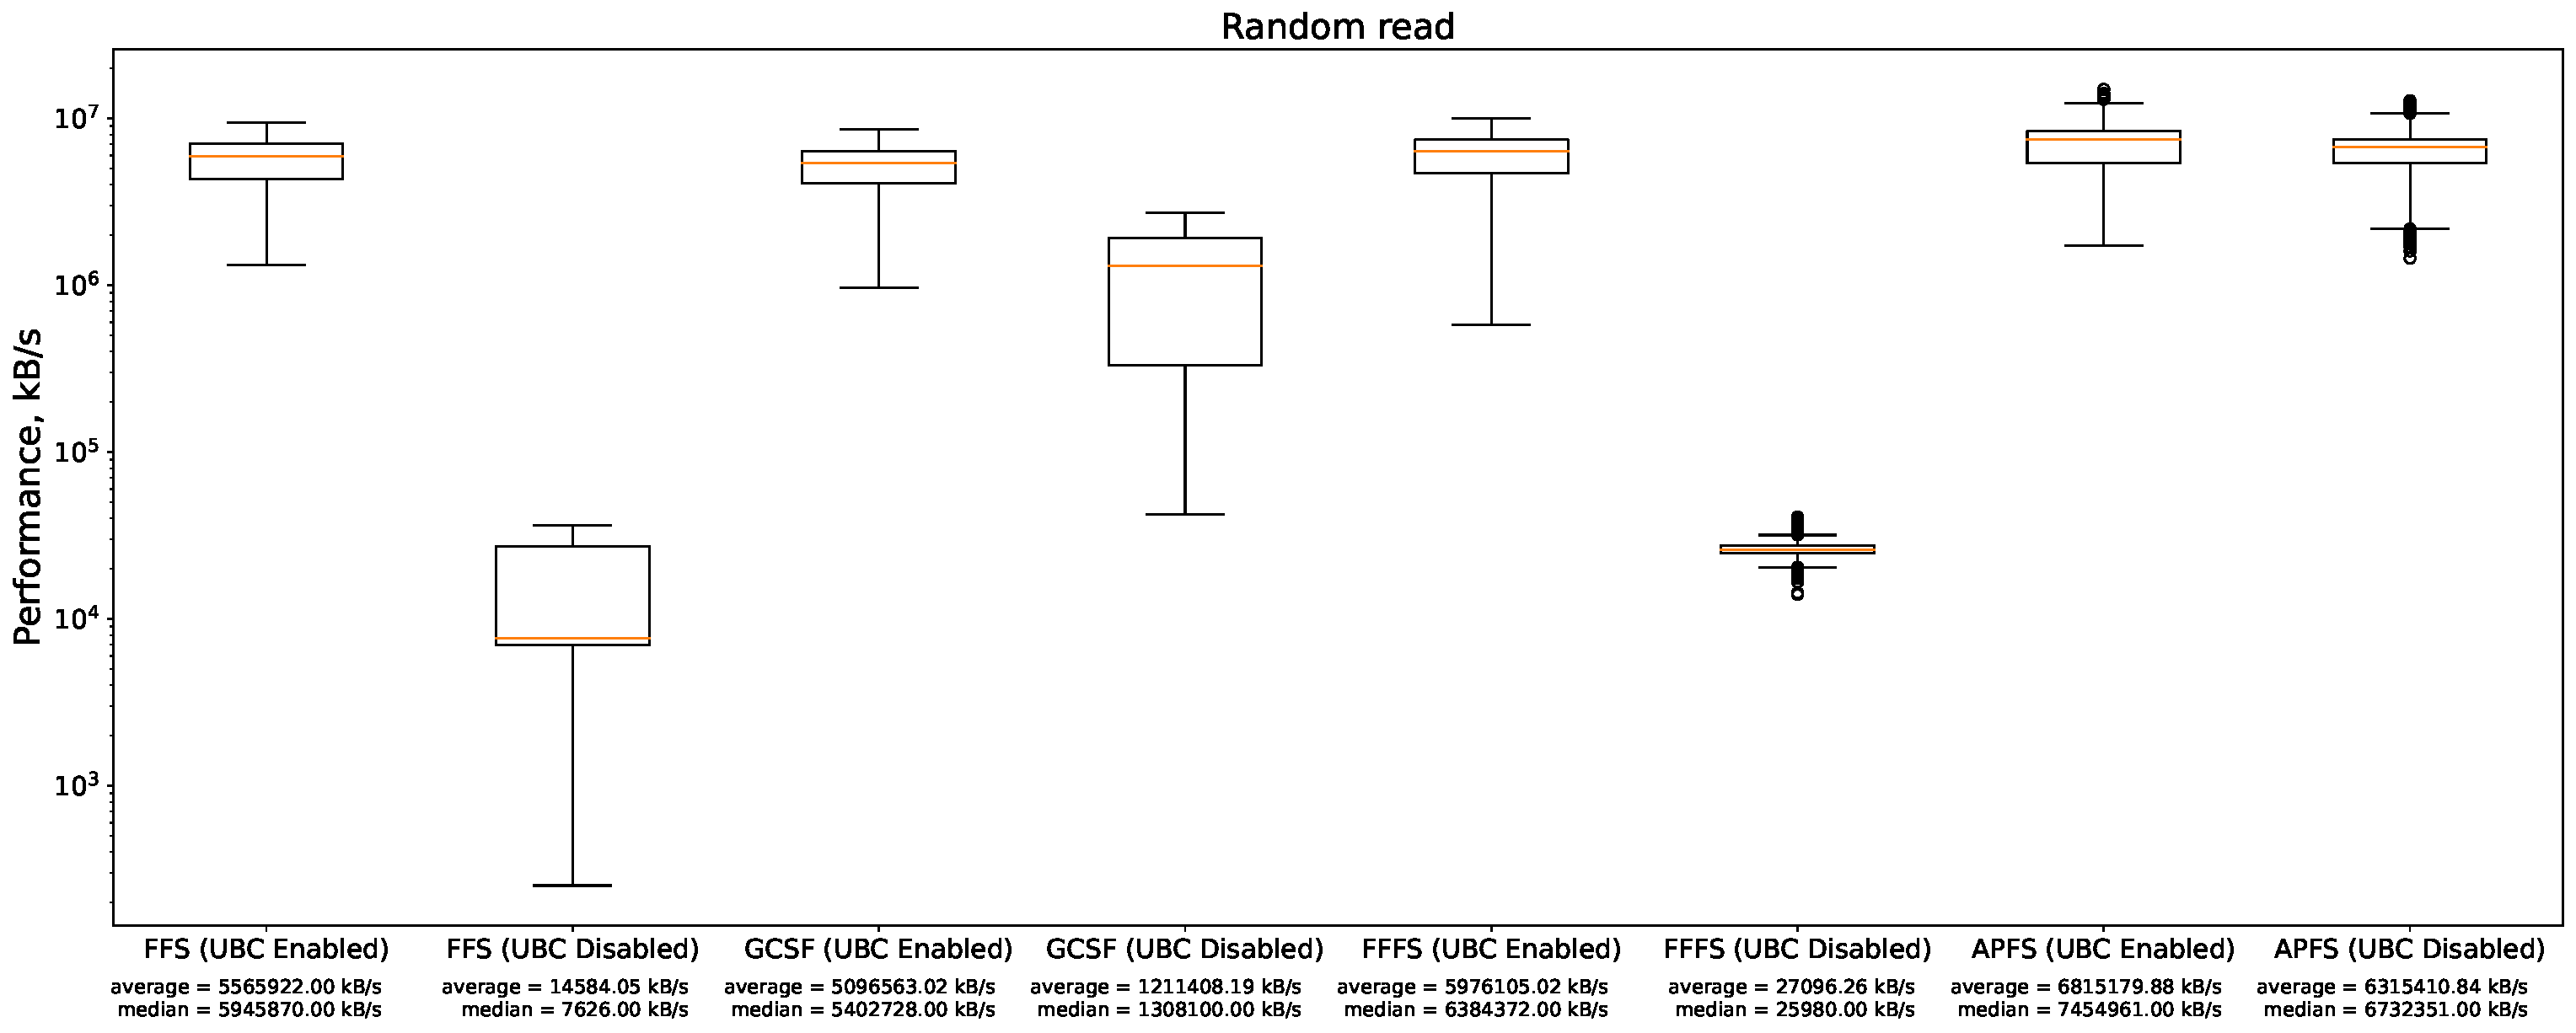
\includegraphics[width=1.0\textwidth]{figures.nosync/benchmarking/Random read-boxplot.pdf}
	\end{center}
	\caption[Box plot of the IOZone output for the Random read test]{Box plot of the IOZone output for the Random read test on the different filesystems}
\end{sidewaysfigure}

\FloatBarrier

Figure~\ref{fig:res_box_rndwrite} presents a box plot for the Random read test for the different filesystems.The results are similar to the results for the \mbox{Re-Write} test presented in Figure~\ref{fig:res_box_rewrite}.

\begin{sidewaysfigure}[!ht]
	\label{fig:res_box_rndwrite}
	\begin{center}
		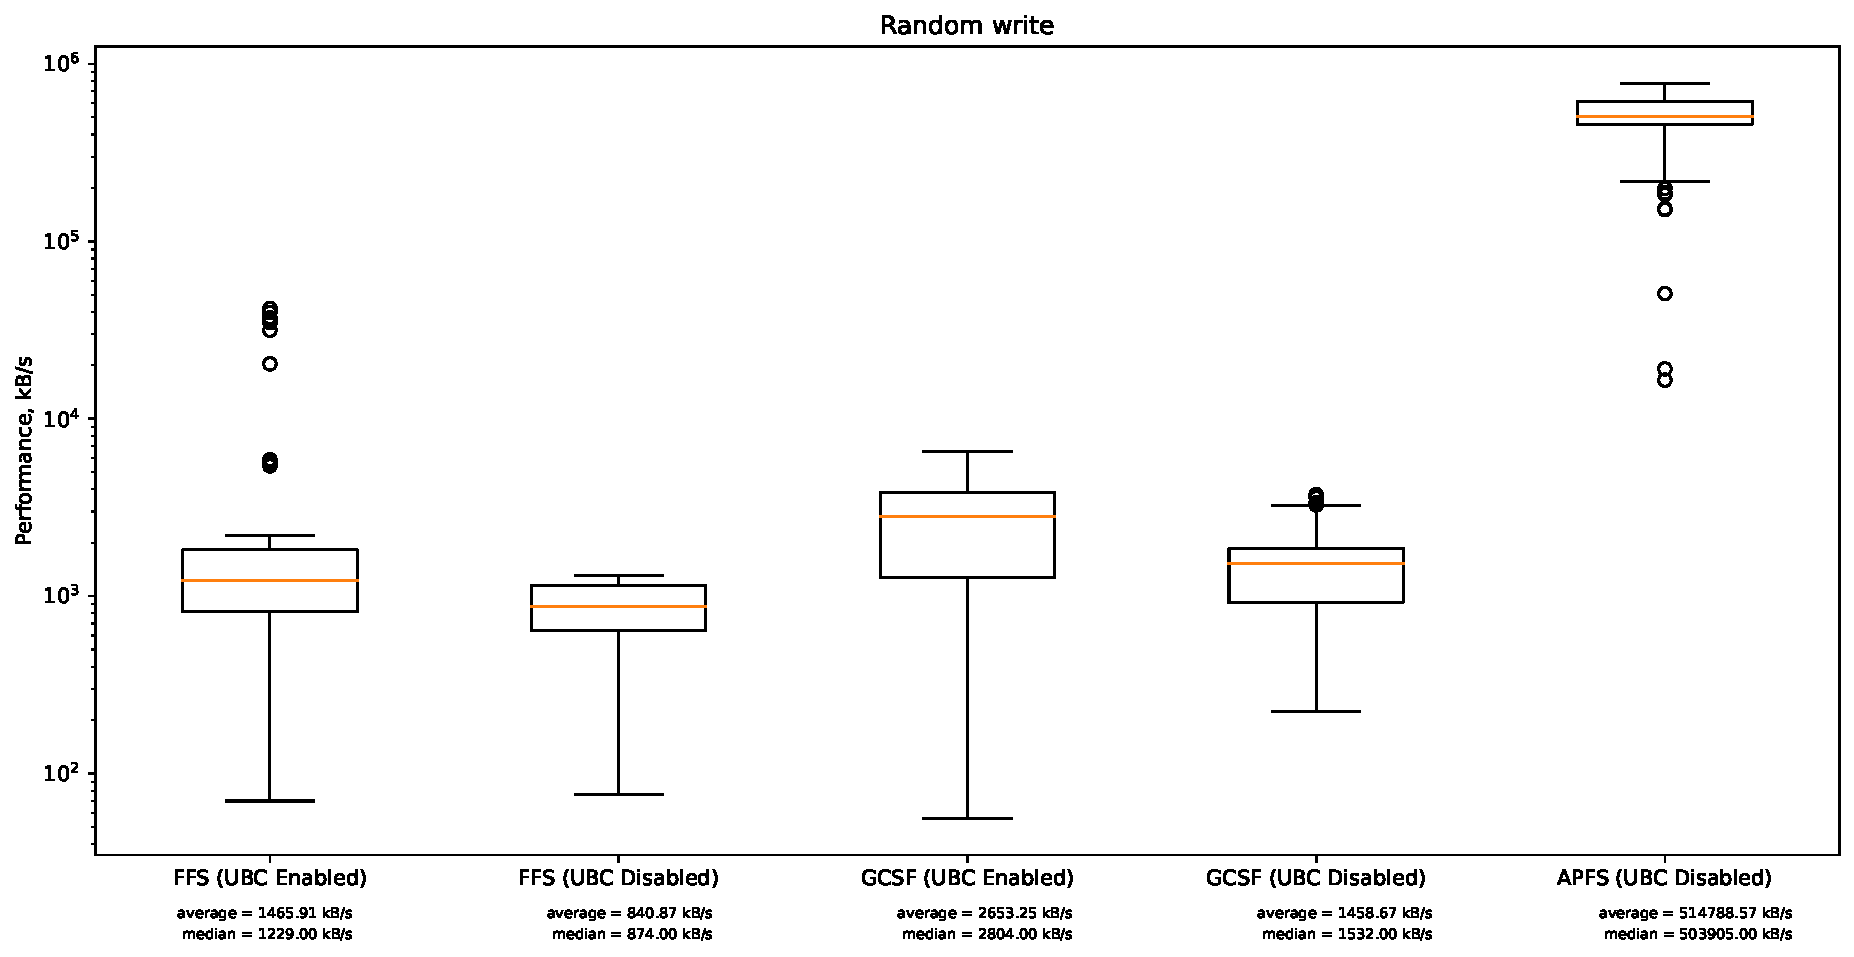
\includegraphics[width=1.0\textwidth]{figures.nosync/benchmarking/Random write-boxplot.pdf}
	\end{center}
	\caption[Box plot of the IOZone output for the Random write test]{Box plot of the IOZone output for the Random write test on the different filesystems}
\end{sidewaysfigure}

\FloatBarrier
\clearpage

Following are histograms for each filesystem and each state of the \gls{UBC}. Each histogram presents the performance distribution for each file size in each file operation test. \Cref{fig:bench_ffs_with_cache} and \Cref{fig:bench_ffs_without_cache} present the performance of \gls{FFS} with the \gls{UBC} enabled and disabled, respectively. \Cref{fig:bench_gcsf_with_cache} and \Cref{fig:bench_gcsf_without_cache} present the performance of \gls{GCSF} with the \gls{UBC} enabled and disabled, respectively. \Cref{fig:bench_fffs_with_cache} and \Cref{fig:bench_fffs_without_cache} present the performance of \gls{FFFS} with the \gls{UBC} enabled and disabled, respectively. \Cref{fig:bench_apfs_with_cache} and \Cref{fig:bench_apfs_without_cache} present the performance of \gls{APFS} with the \gls{UBC} enabled and disabled, respectively. The distribution patterns varies greatly for the different filesystems and the state of the \gls{UBC}. For instance, for \gls{FFS} with the \gls{UBC} enabled, most bars are on the same side of the graph for the write tests, while for \gls{FFS} with the \gls{UBC} disabled, the different file sizes show a pattern similar to a bell curve. The difference in the histograms indicate that the distribution of values differs greatly between the filesystems and the different states of the \gls{UBC}. The write tests for \gls{FFS}, \gls{GCSF}, and \gls{FFS}, all with the \gls{UBC} disabled, all look normally distributed when looking at each file size individually. \gls{FFFS} with the \gls{UBC} disabled also look to follow a normal distribution for each file size individually. No histogram show a normal distribution for all the values.
\clearpage

\begin{figure}[!htb]
	\label{fig:bench_ffs_with_cache}
	\begin{center}
		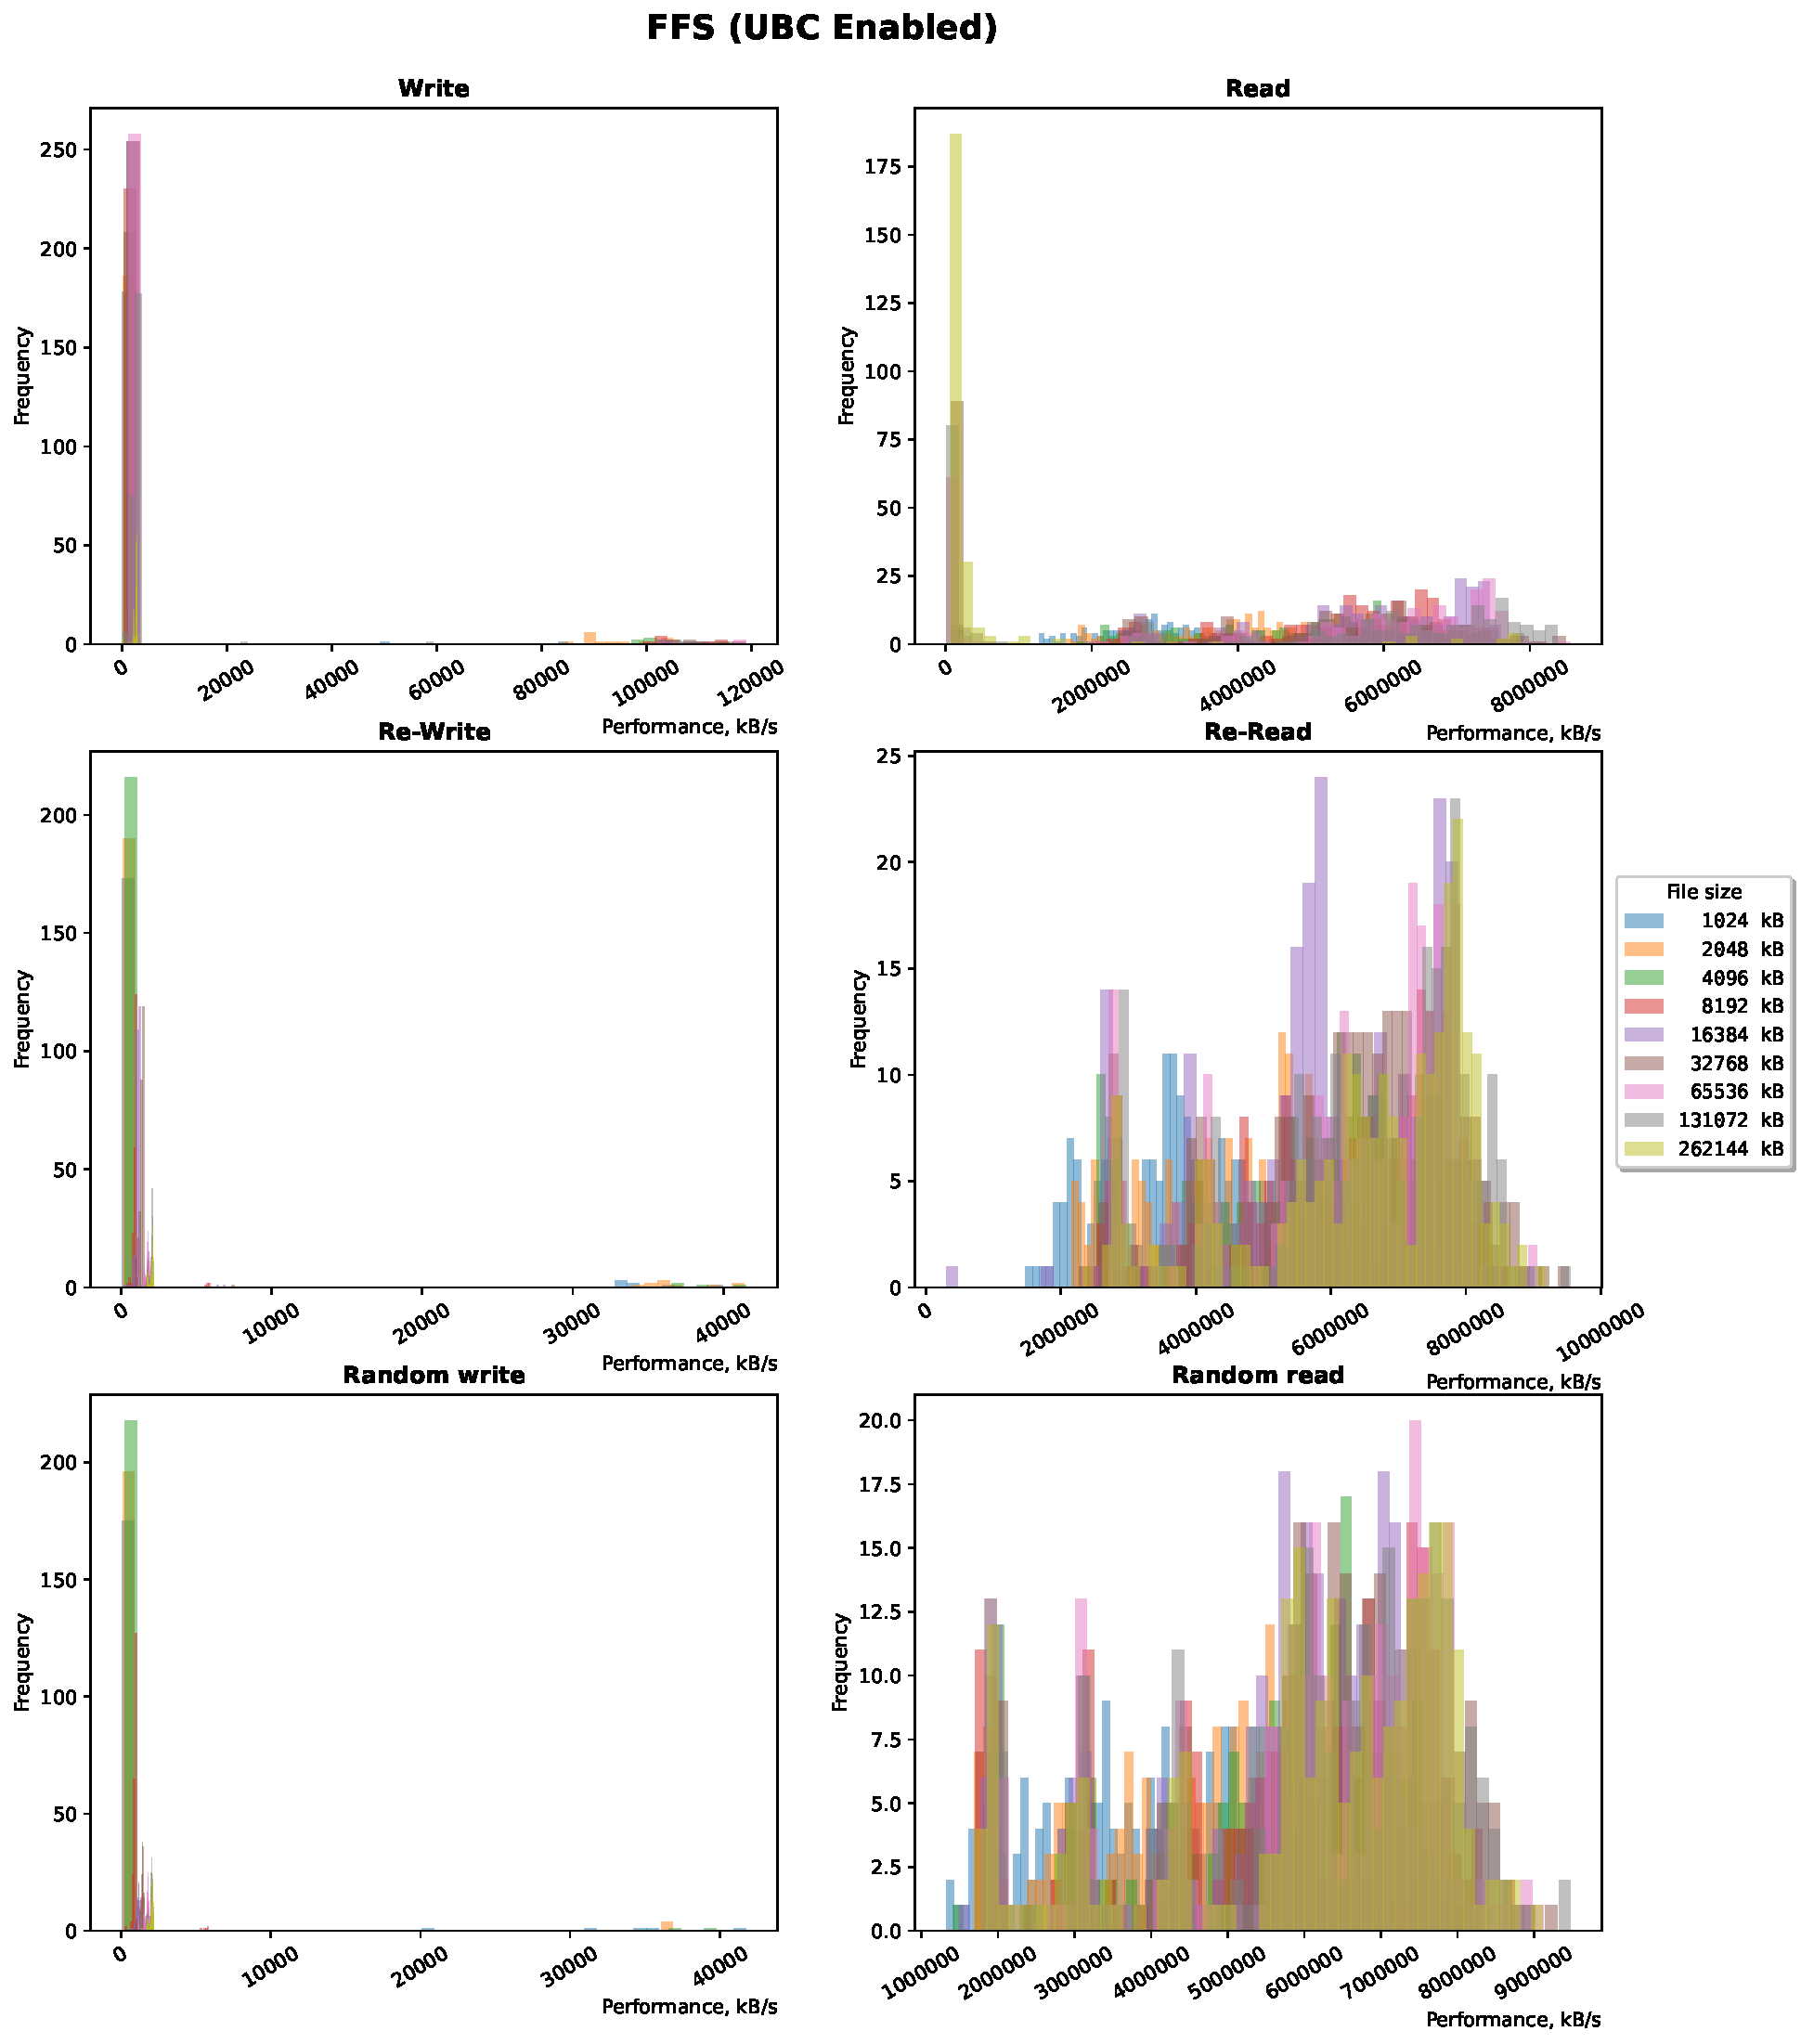
\includegraphics[width=1.2\textwidth]{figures.nosync/benchmarking/FFS/FFS-UBC Enabled-hist.pdf}
	\end{center}
	\caption[Performance comparison for FFS with the UBC enabled]{Performance comparison of different file sizes for FFS with the UBC enabled}
\end{figure}
\clearpage
\begin{figure}[!htb]
	\label{fig:bench_ffs_without_cache}
	\begin{center}
		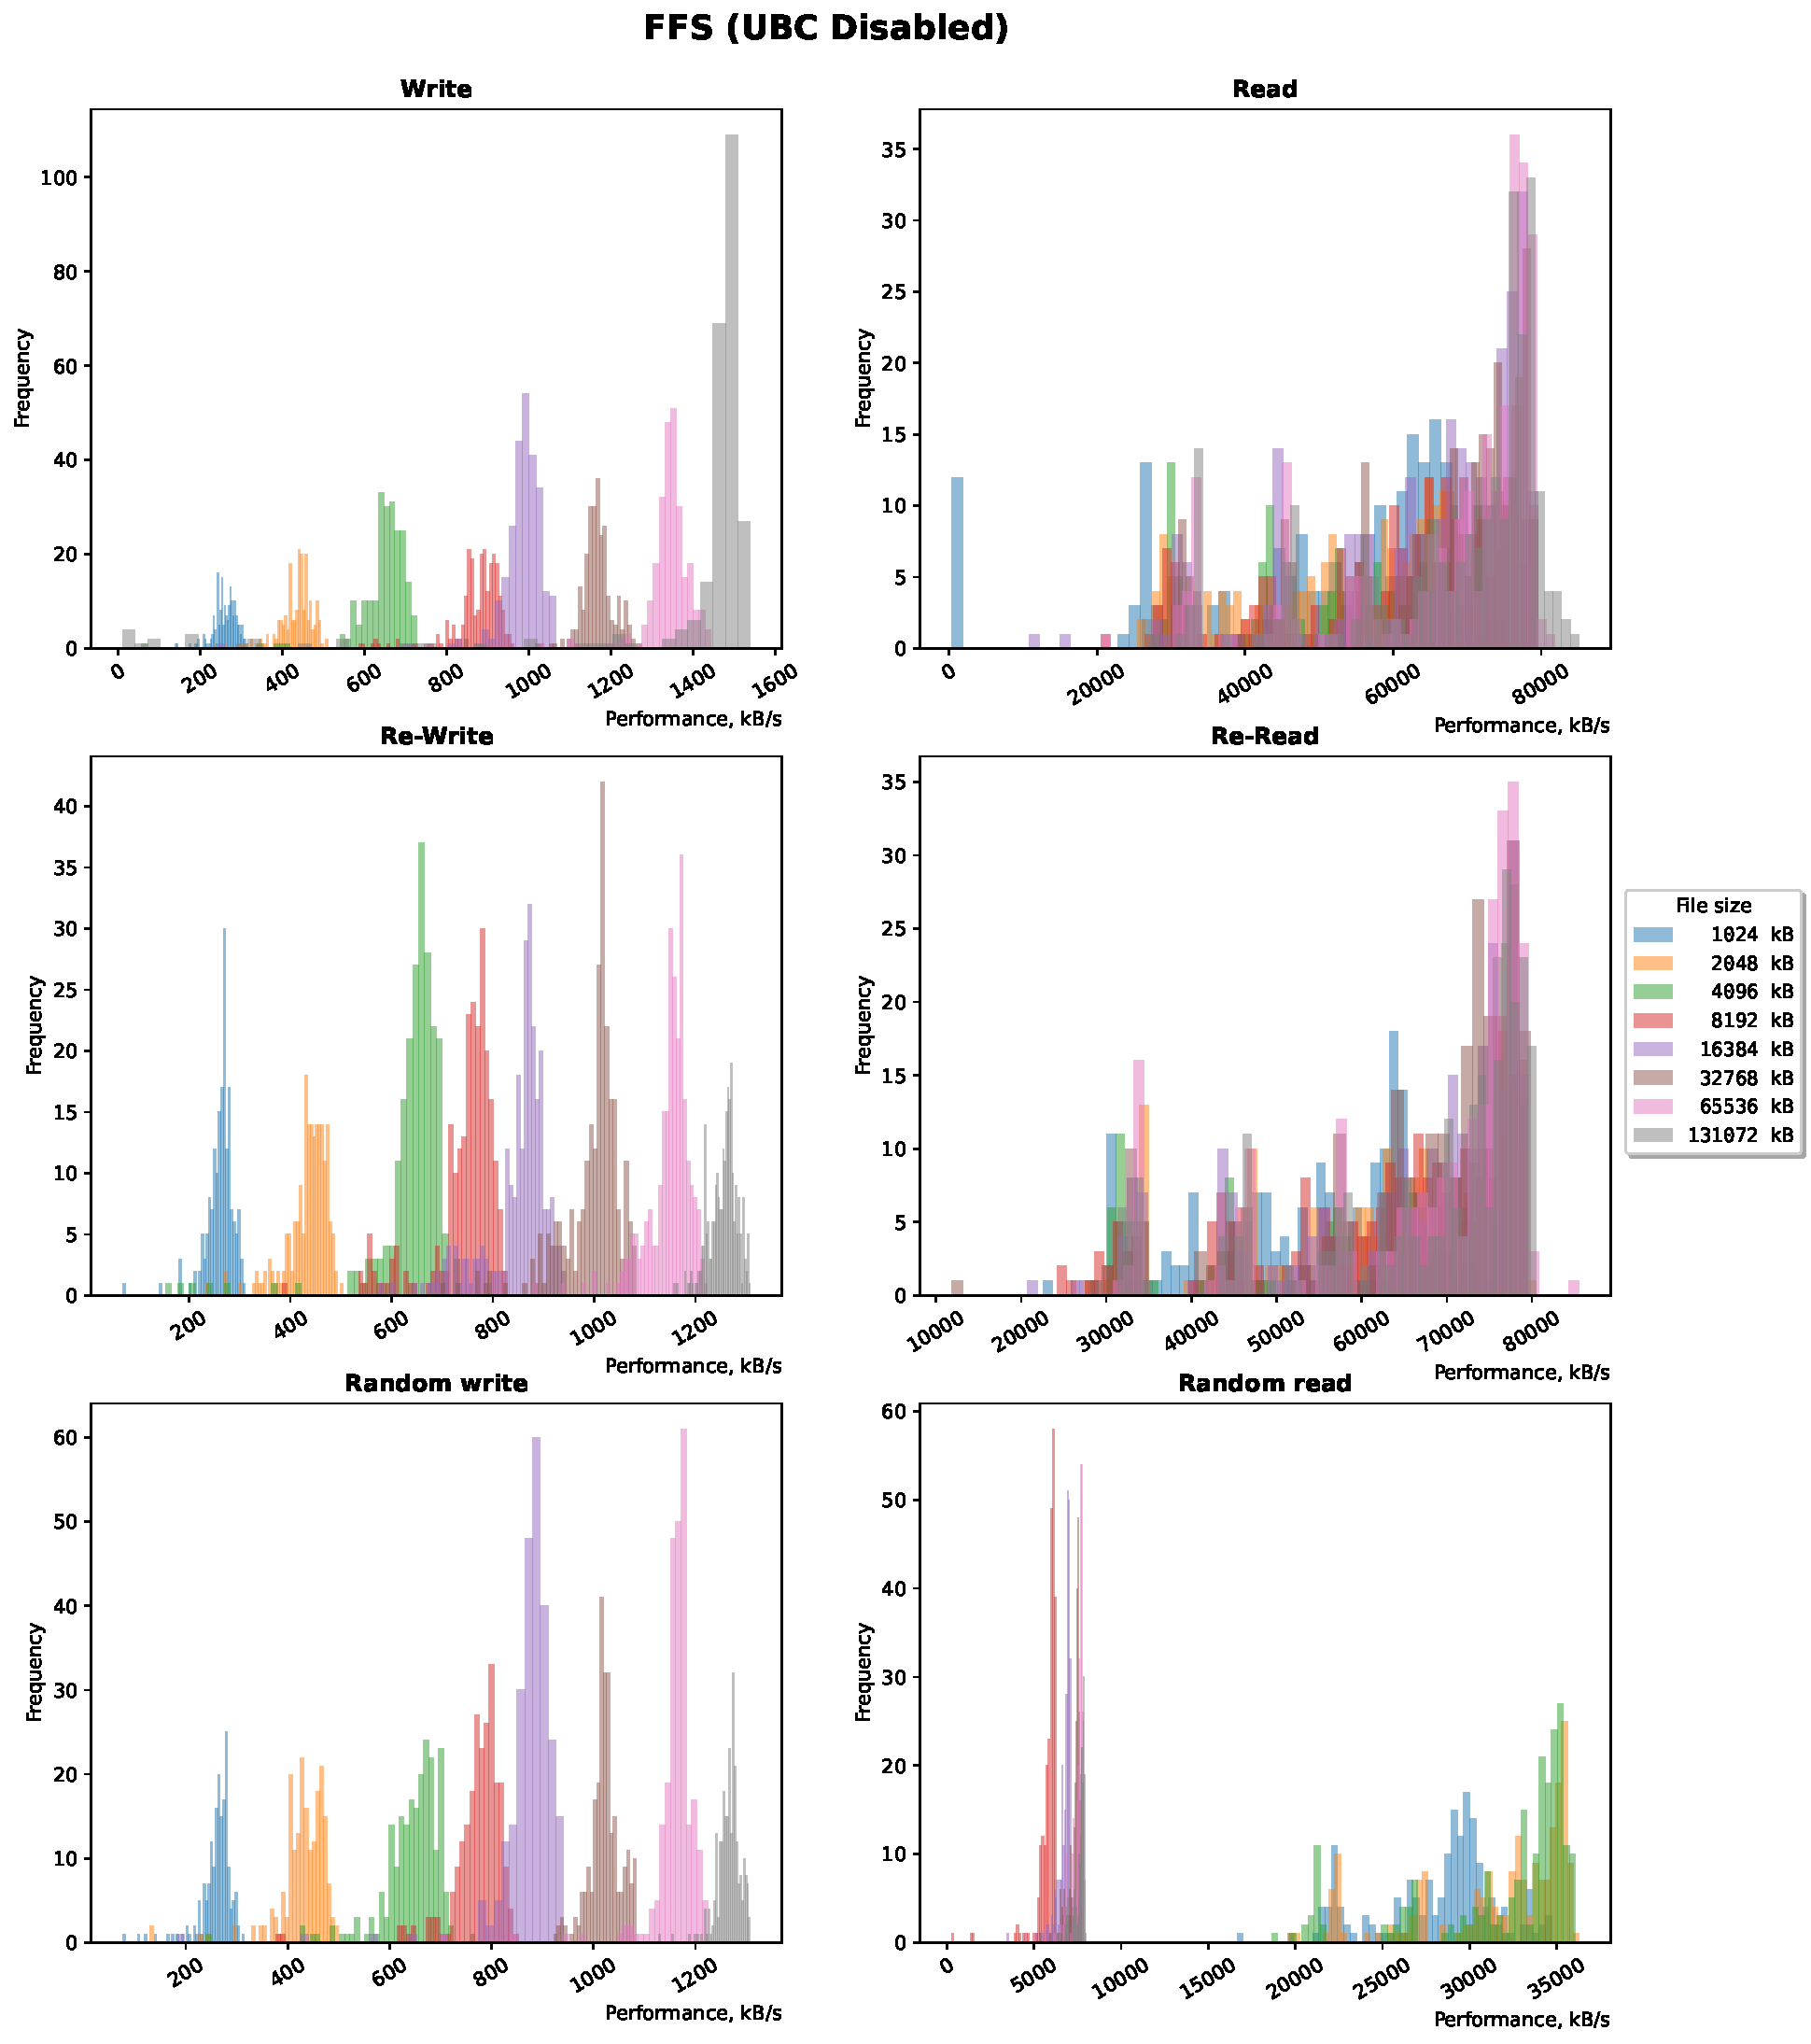
\includegraphics[width=1.0\textwidth]{figures.nosync/benchmarking/FFS/FFS-UBC Disabled-hist.pdf}
	\end{center}
	\caption[Performance comparison for FFS with the UBC disabled]{Performance comparison of different file sizes for FFS with the UBC disabled}
\end{figure}
\clearpage


\begin{figure}[!htb]
	\label{fig:bench_gcsf_with_cache}
	\begin{center}
		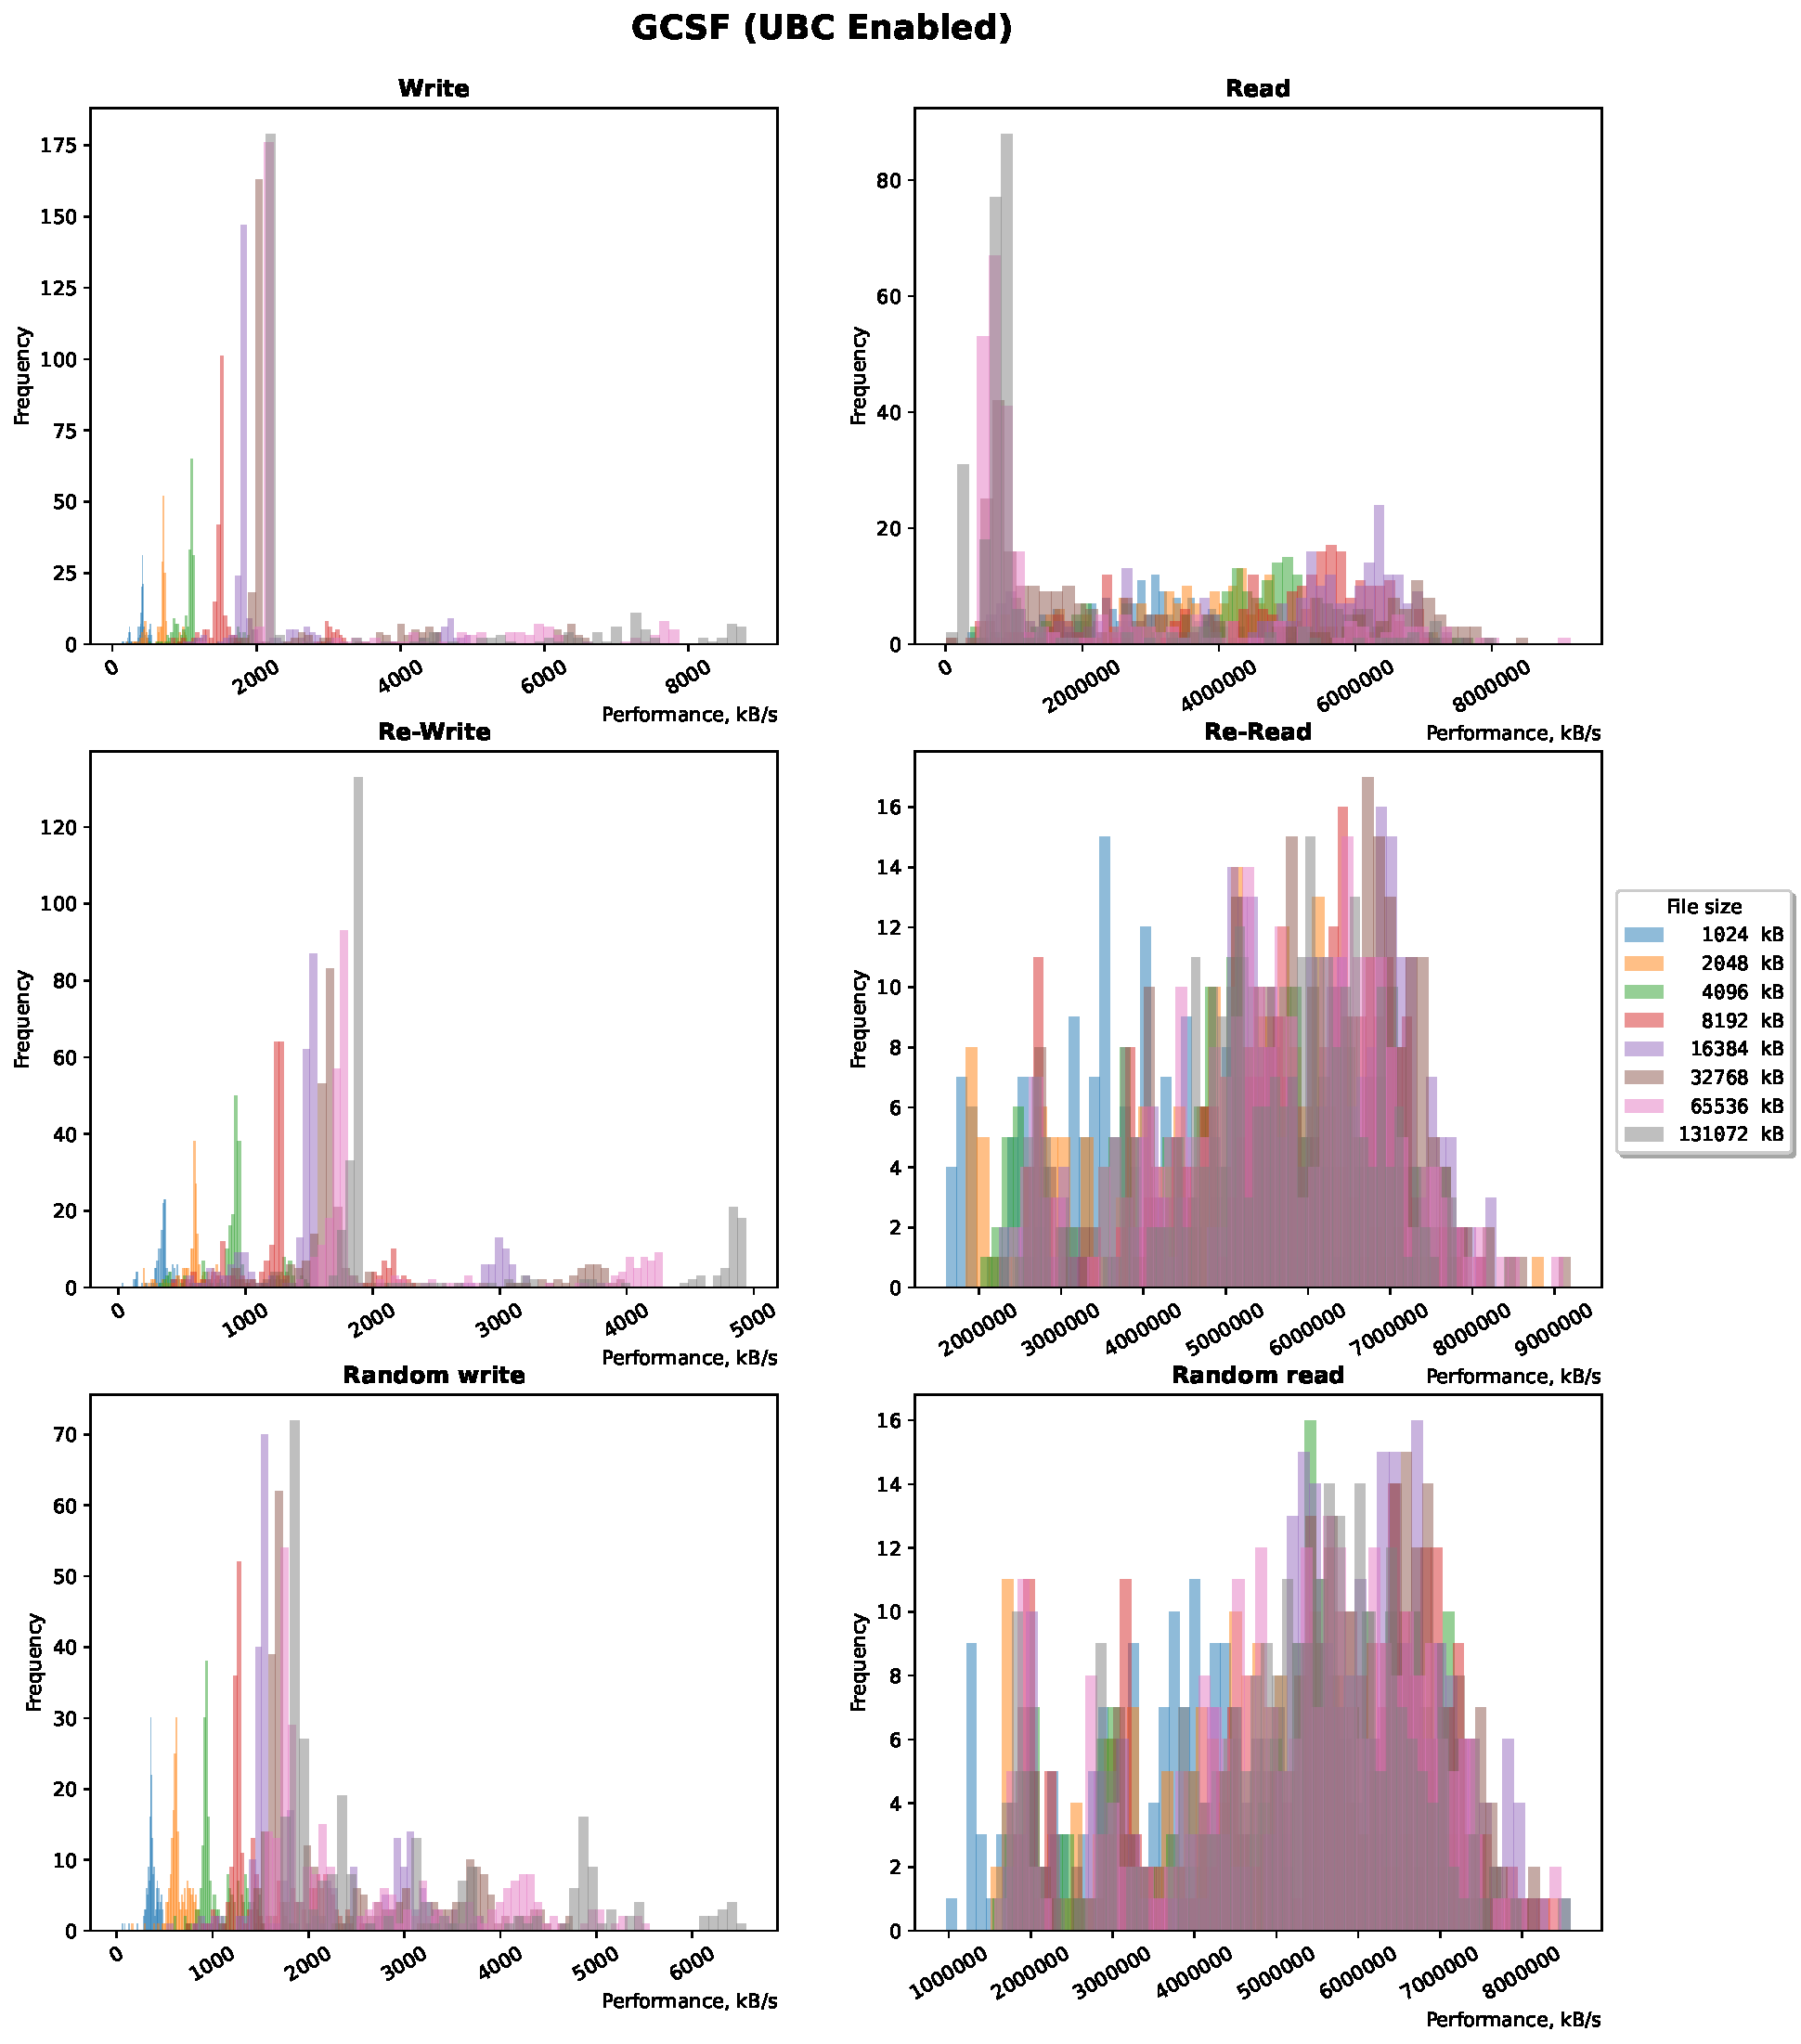
\includegraphics[width=1.0\textwidth]{figures.nosync/benchmarking/GCSF/GCSF-UBC Enabled-hist.pdf}
	\end{center}
	\caption[Performance comparison for GCSF with the UBC enabled]{Performance comparison of different file sizes for GCSF with the UBC enabled}
\end{figure}
\clearpage
\begin{figure}[!htb]
	\label{fig:bench_gcsf_without_cache}
	\begin{center}
		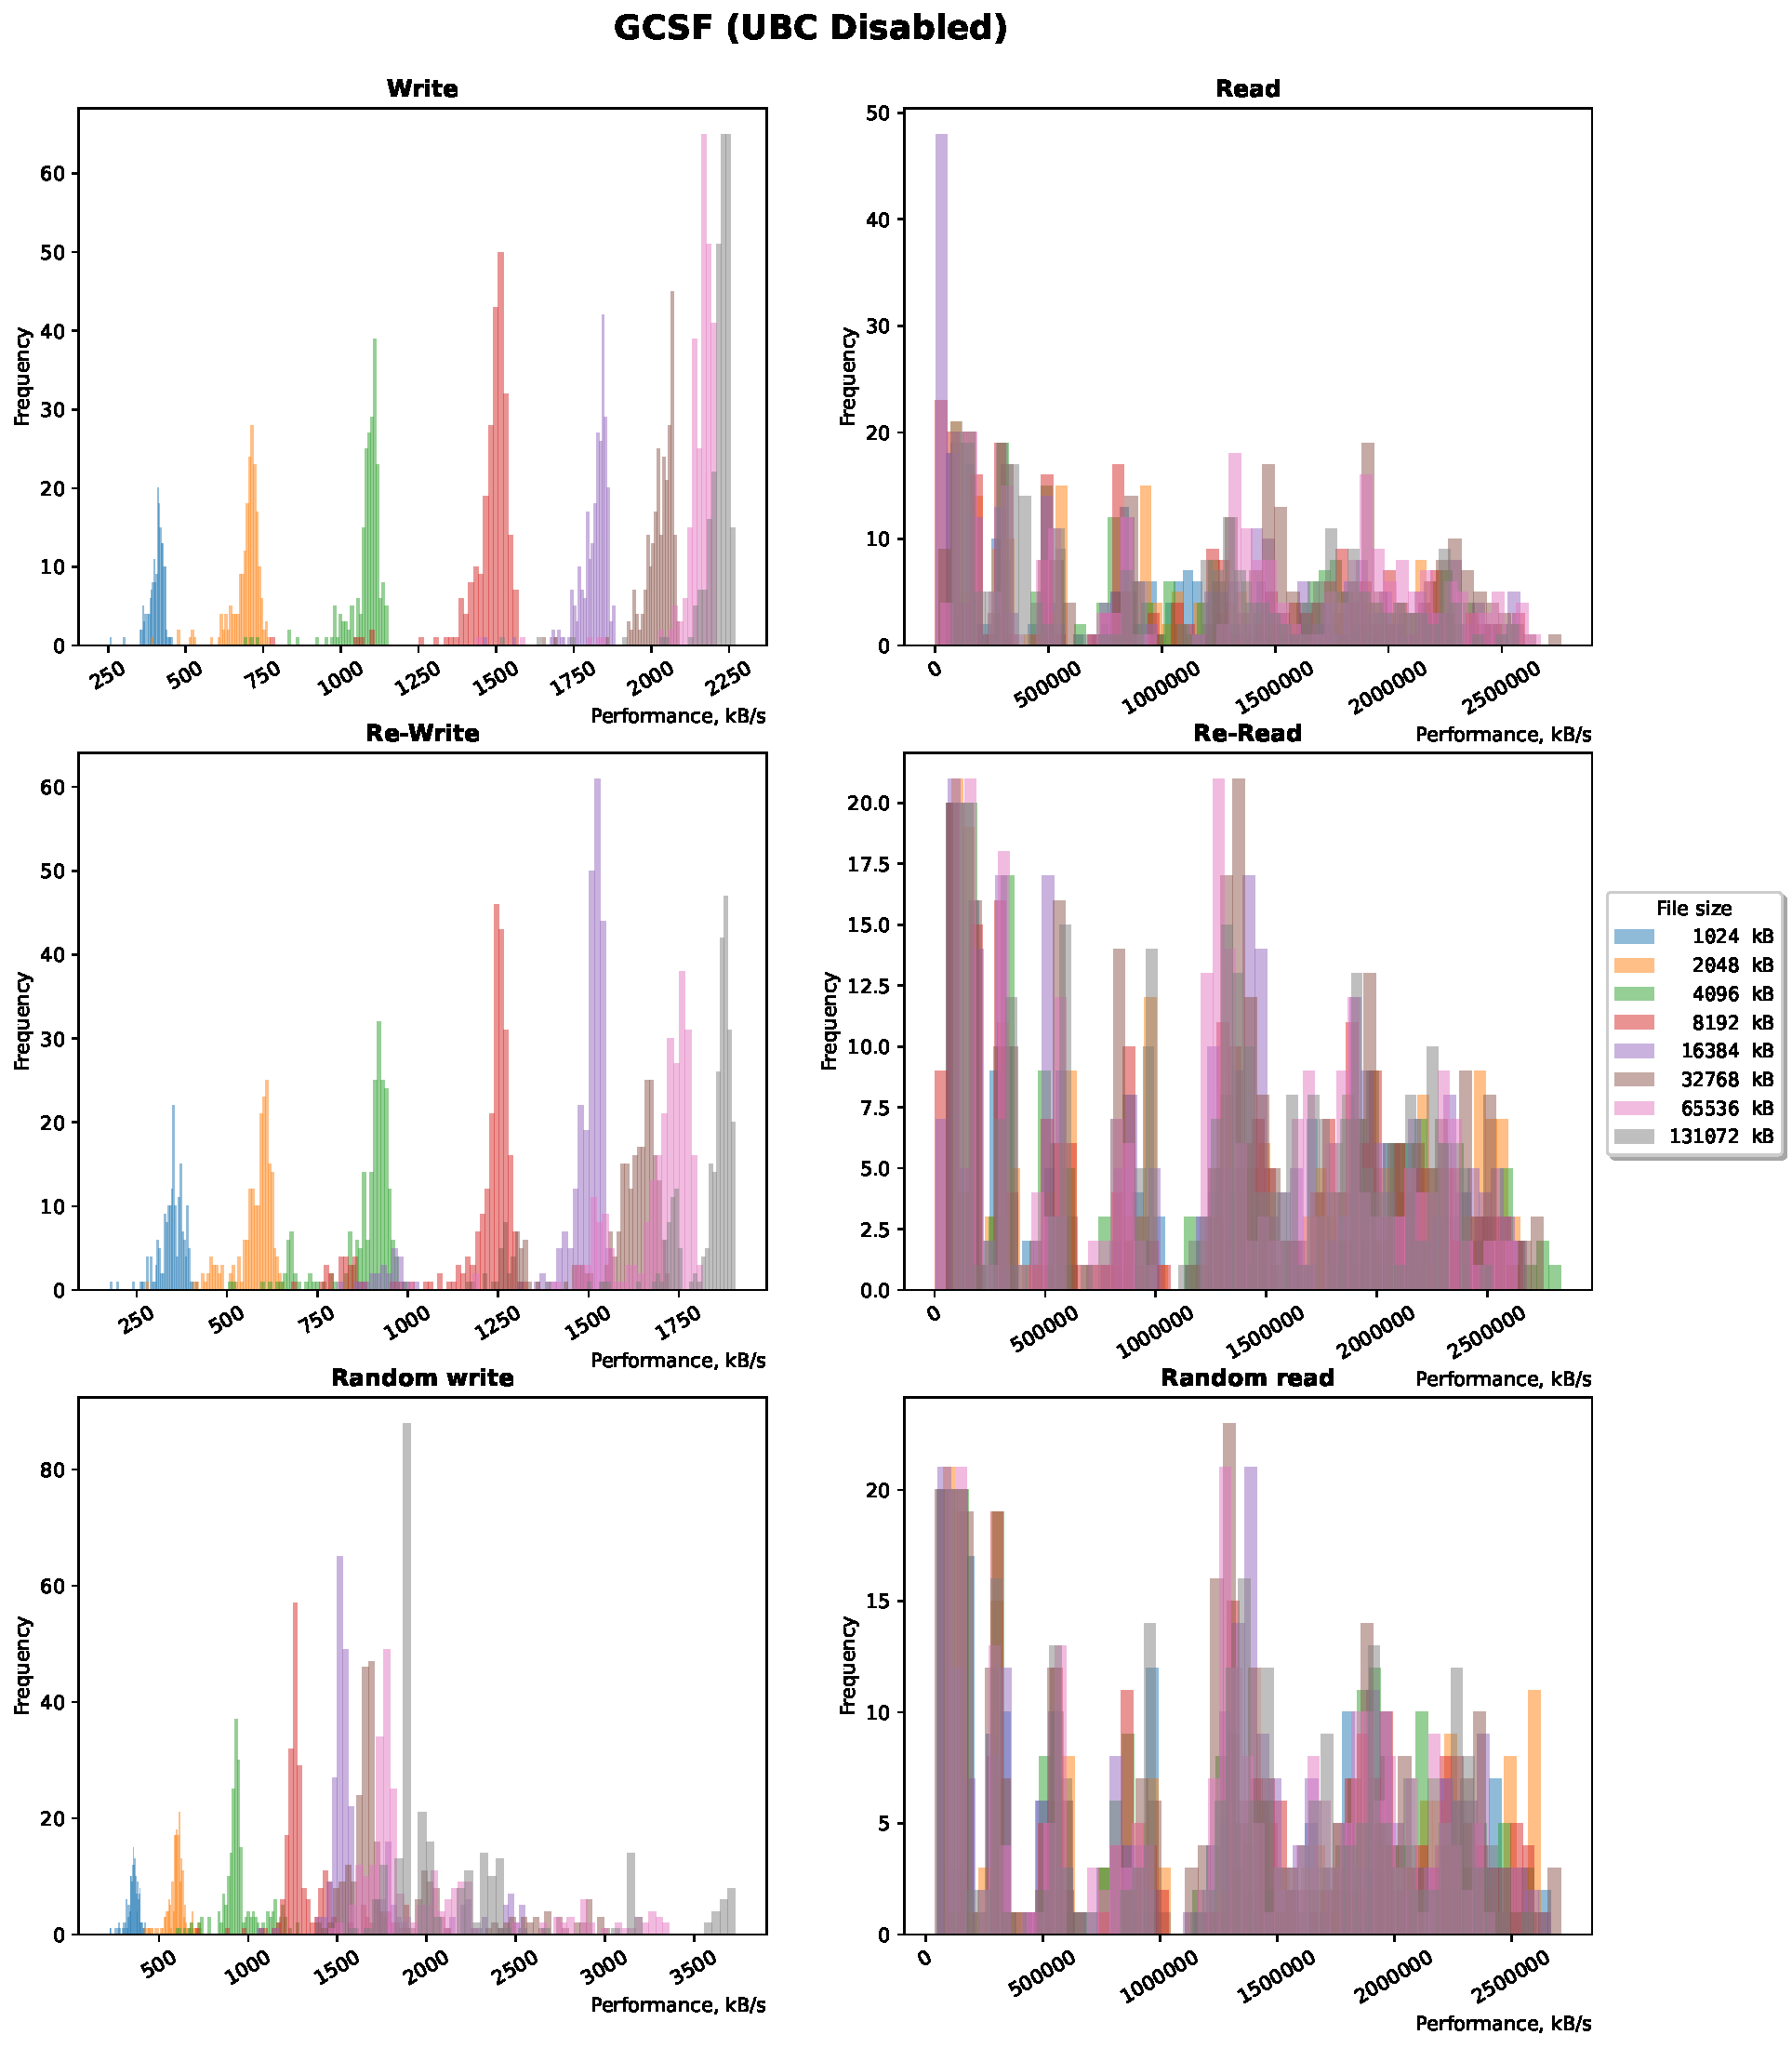
\includegraphics[width=1.0\textwidth]{figures.nosync/benchmarking/GCSF/GCSF-UBC Disabled-hist.pdf}
	\end{center}
	\caption[Performance comparison for GCSF with the UBC disabled]{Performance comparison of different file sizes for GCSF with the UBC disabled}
\end{figure}
\clearpage

\begin{figure}[!htb]
	\label{fig:bench_fffs_with_cache}
	\begin{center}
		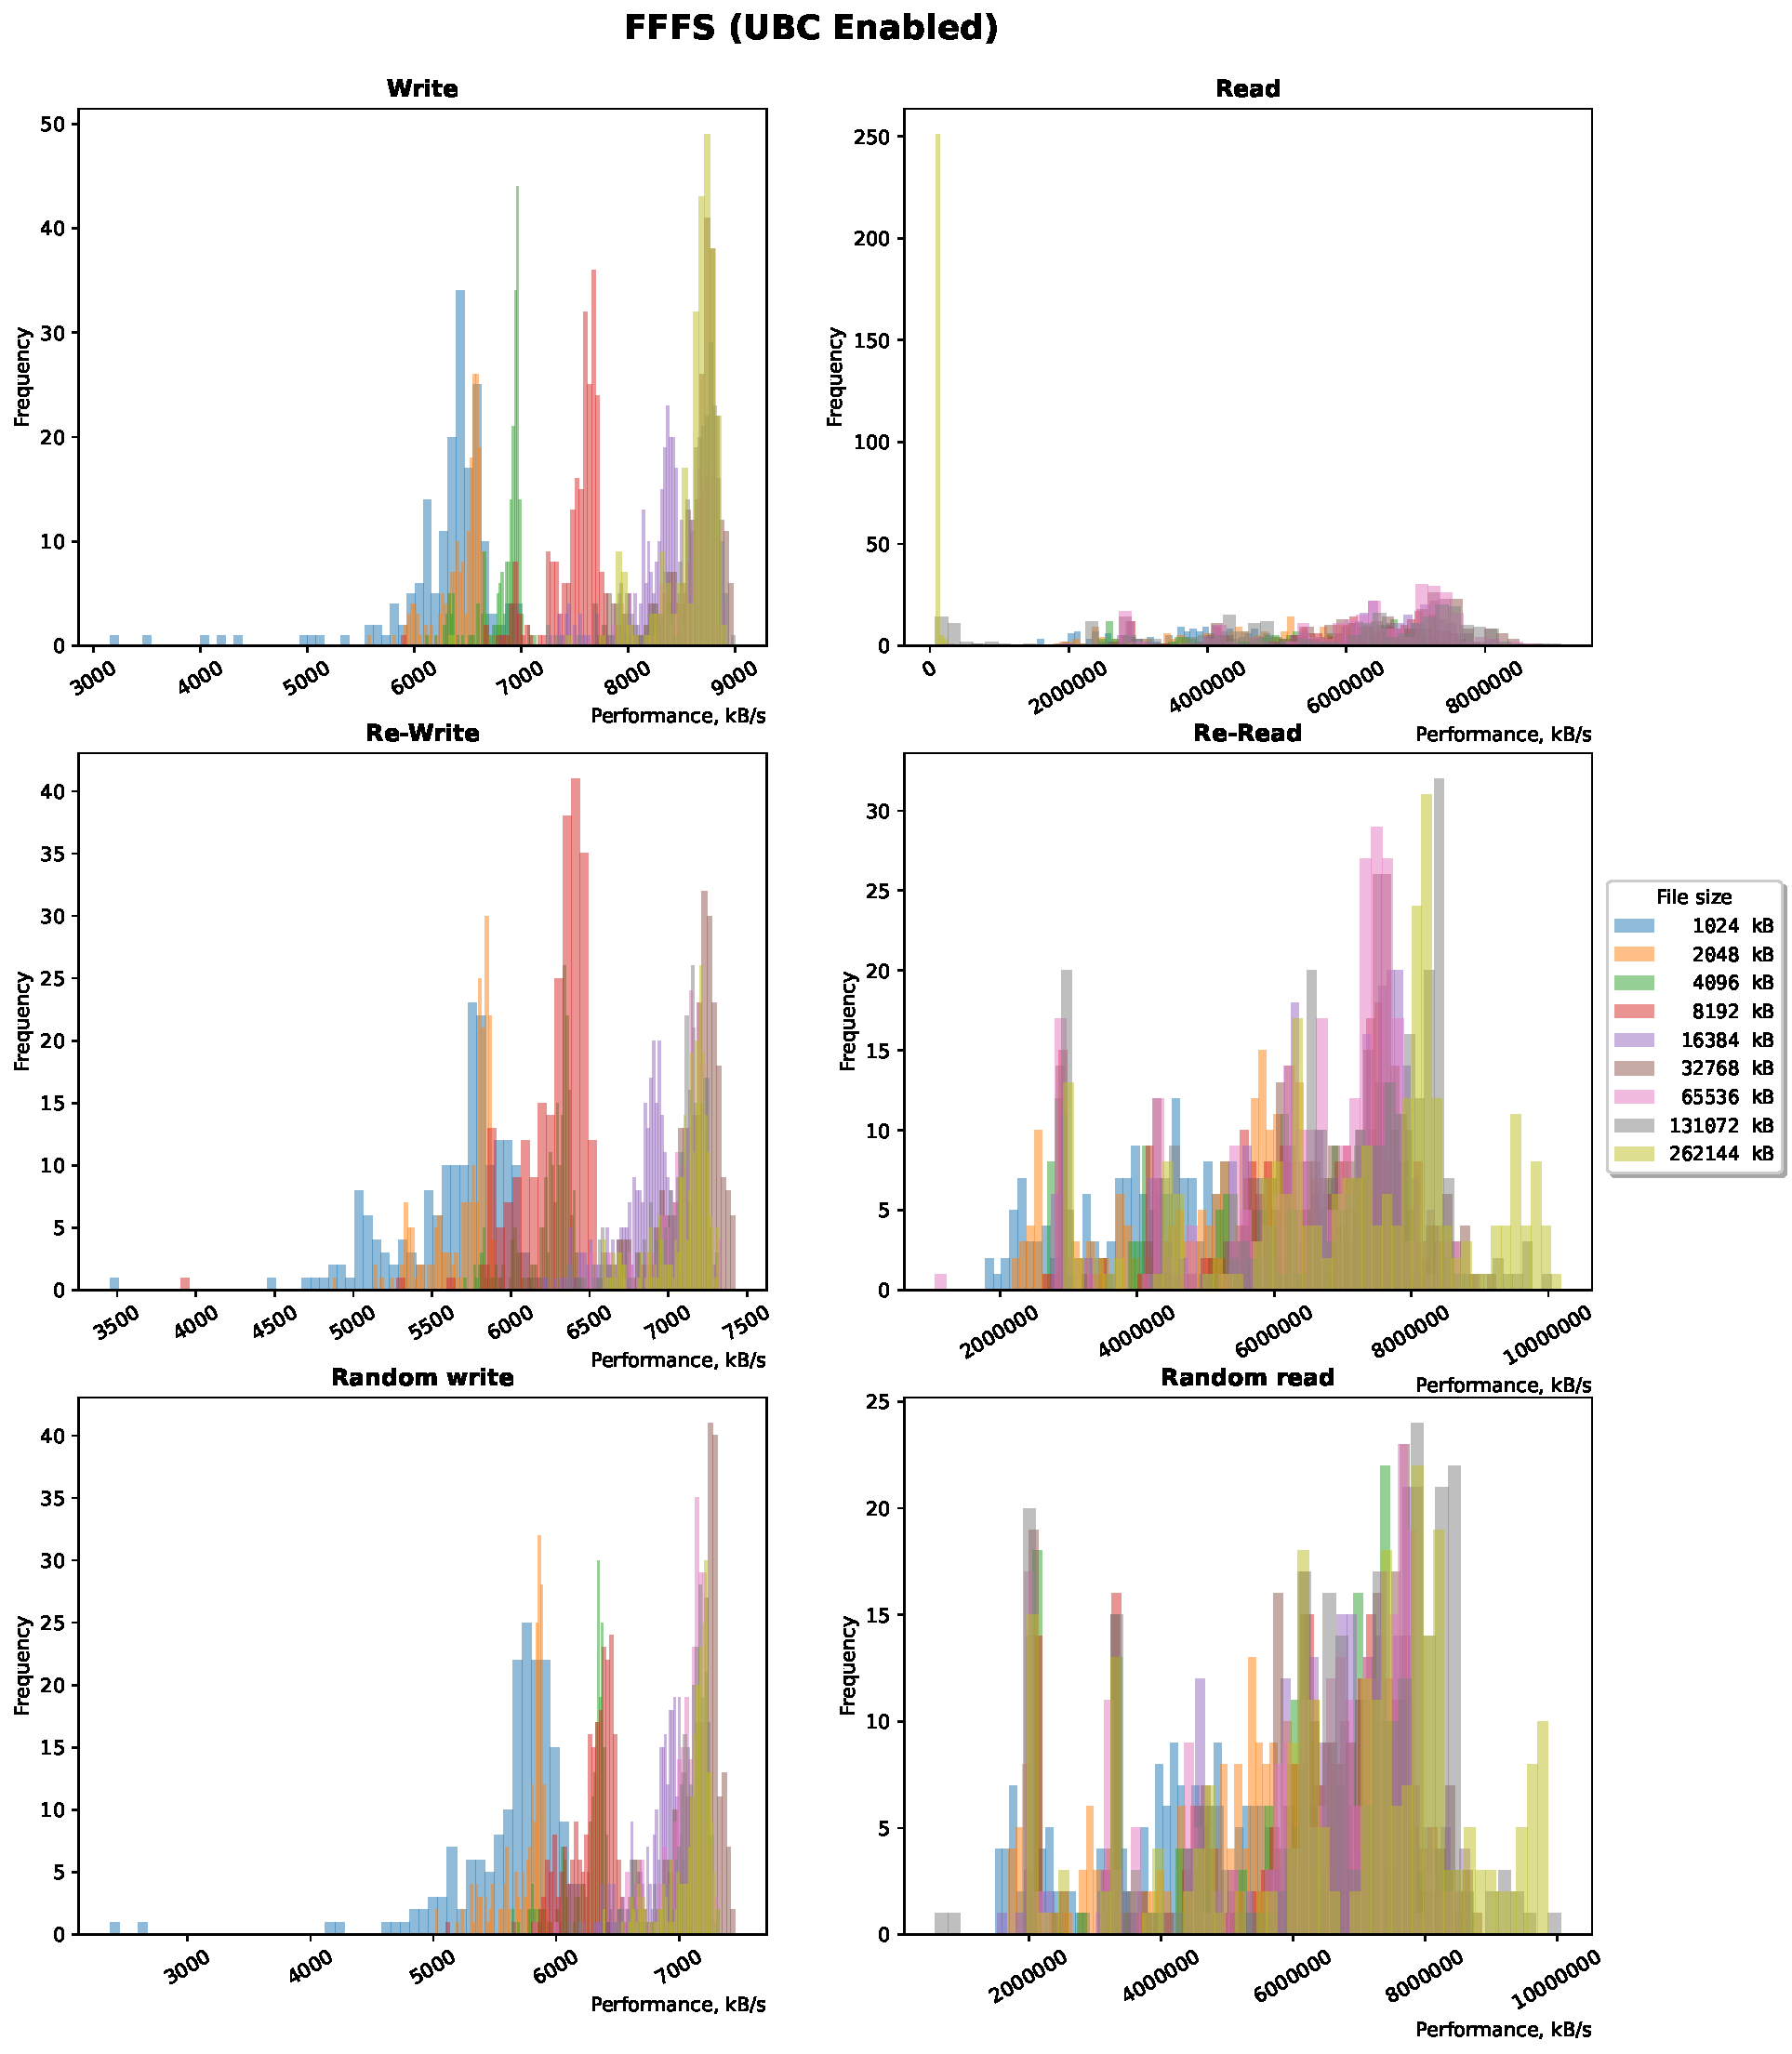
\includegraphics[width=1.0\textwidth]{figures.nosync/benchmarking/FFFS/FFFS-UBC Enabled-hist.pdf}
	\end{center}
	\caption[Performance comparison for FFFS with the UBC enabled]{Performance comparison of different file sizes for FFFS with the UBC enabled}
\end{figure}
\clearpage
\begin{figure}[!htb]
	\label{fig:bench_fffs_without_cache}
	\begin{center}
		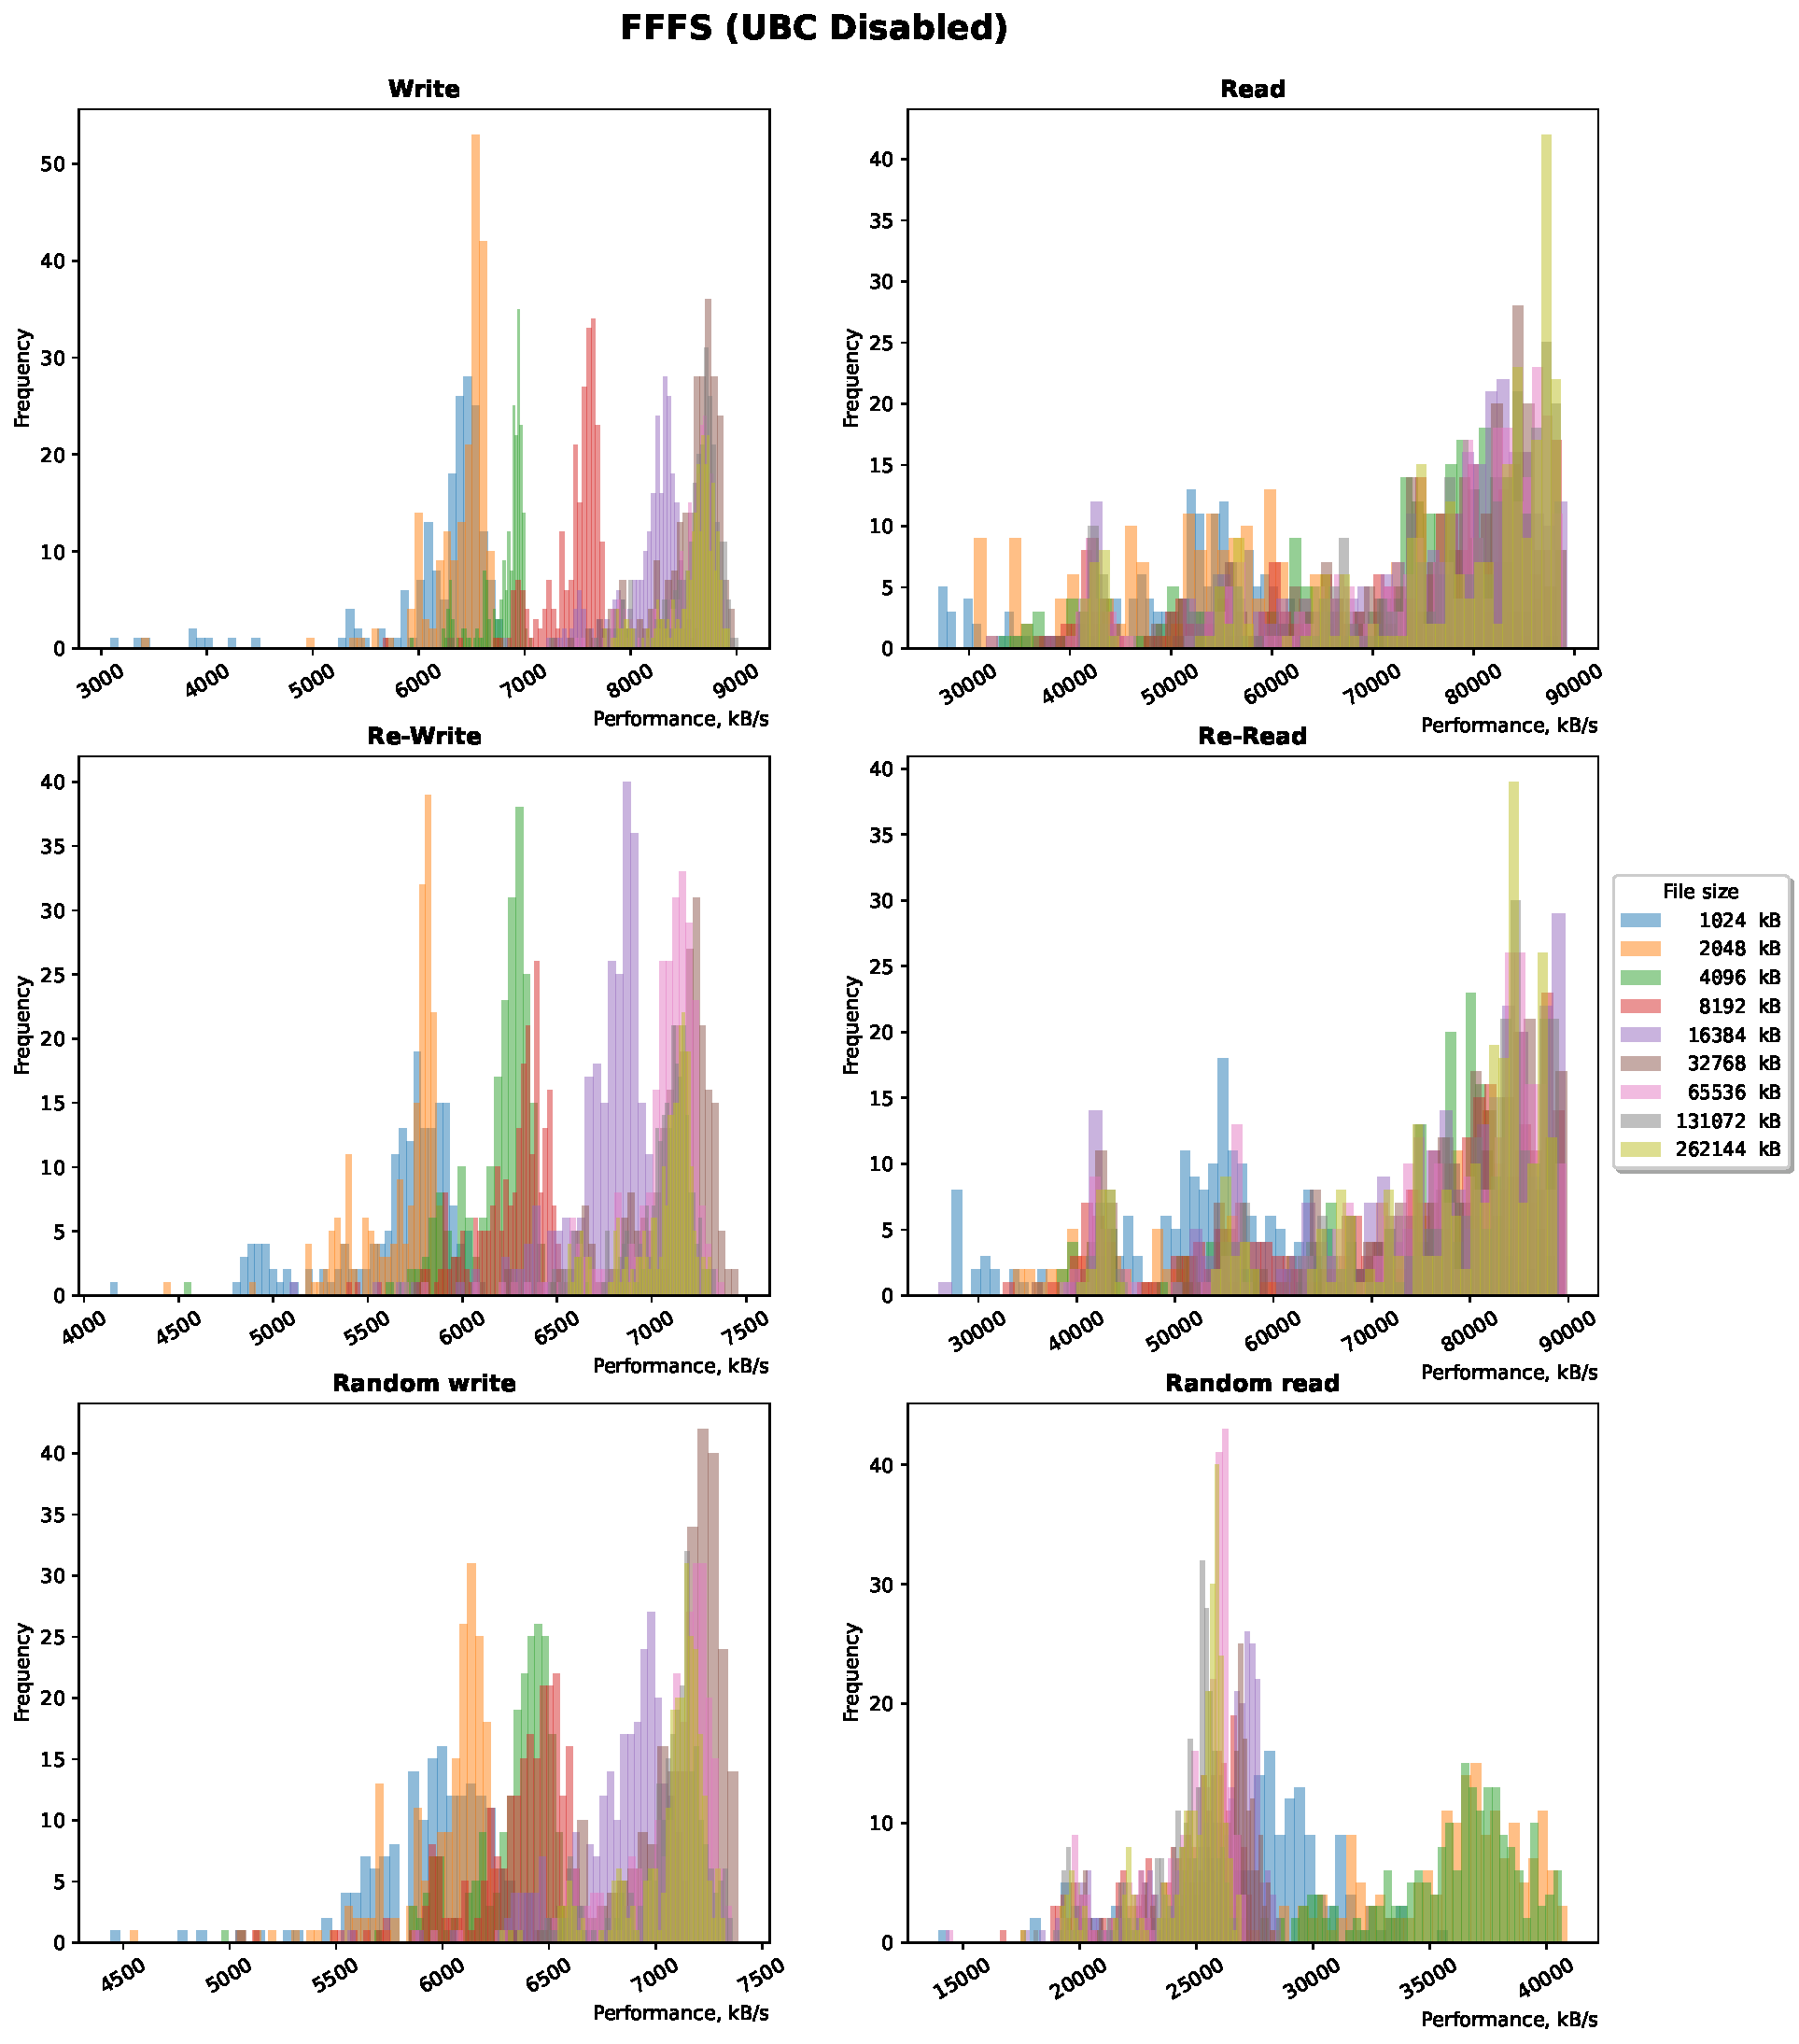
\includegraphics[width=1.0\textwidth]{figures.nosync/benchmarking/FFFS/FFFS-UBC Disabled-hist.pdf}
	\end{center}
	\caption[Performance comparison for FFFS with the UBC disabled]{Performance comparison of different file sizes for FFFS with the UBC disabled}
\end{figure}
\clearpage



\begin{figure}[!htb]
	\label{fig:bench_apfs_with_cache}
	\begin{center}
		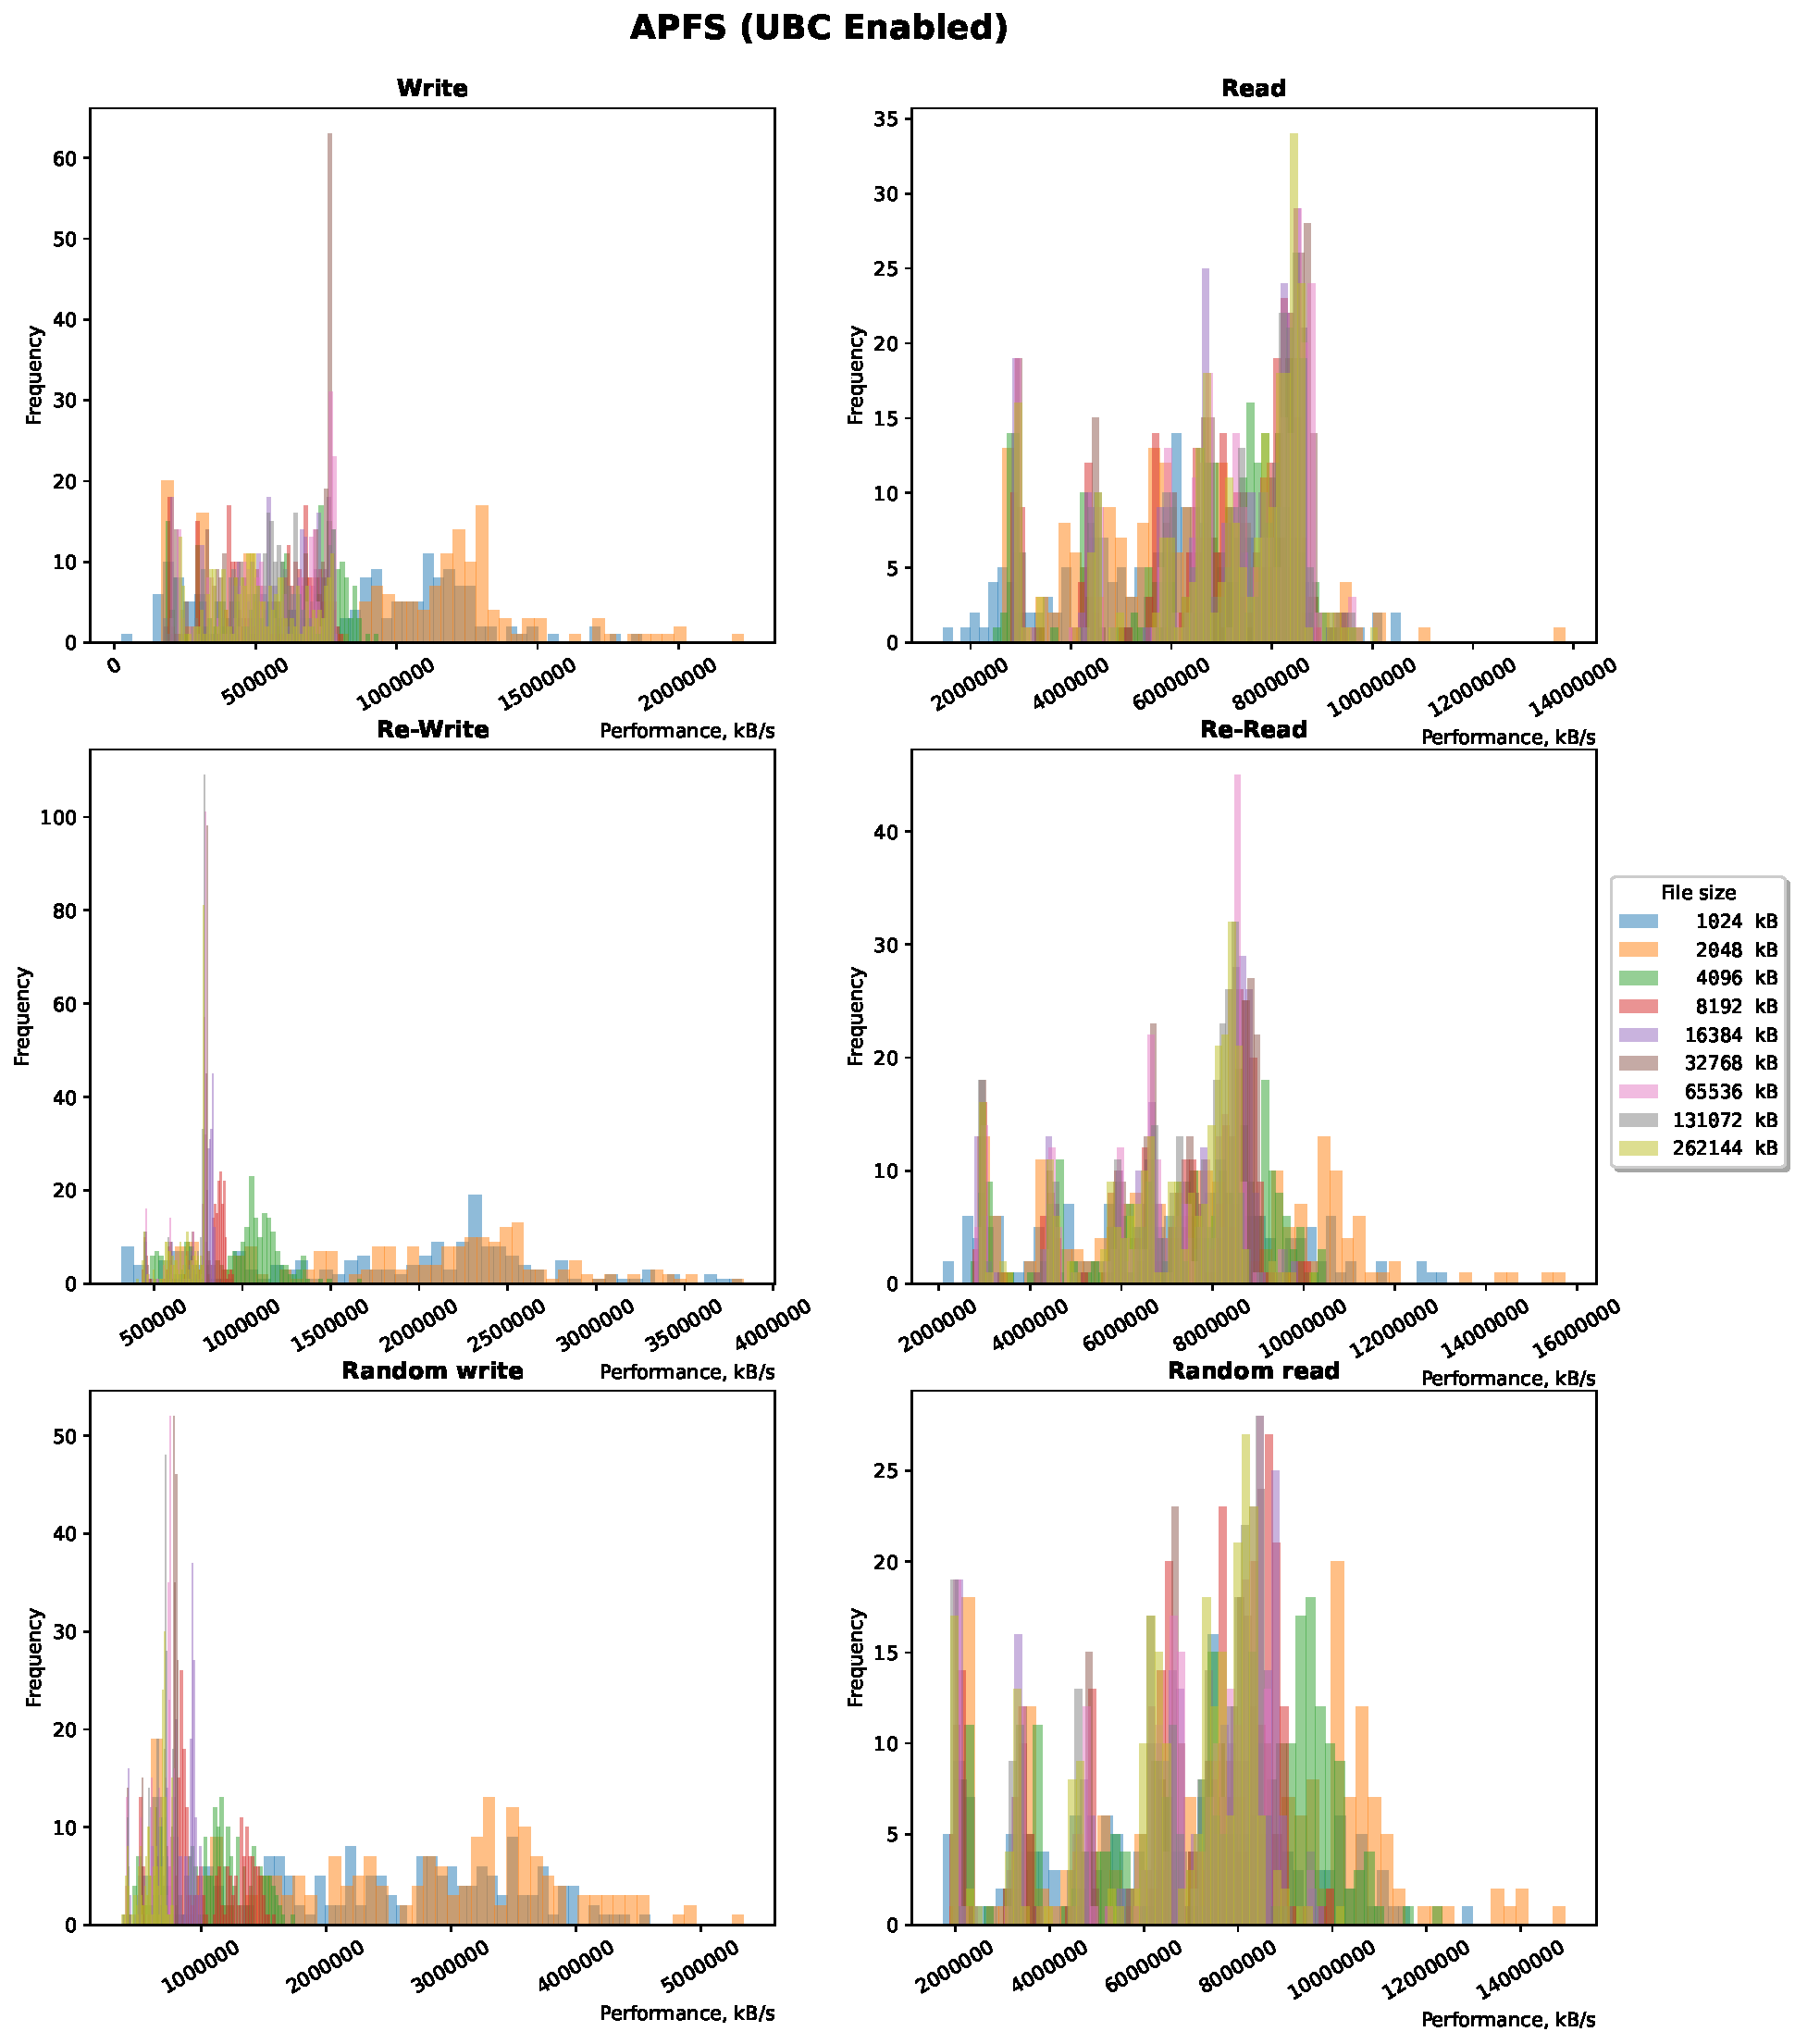
\includegraphics[width=1.0\textwidth]{figures.nosync/benchmarking/APFS/APFS-UBC Enabled-hist.pdf}
	\end{center}
	\caption[Performance comparison for APFS with the UBC enabled]{Performance comparison of different file sizes for APFS with the UBC enabled}
\end{figure}
\clearpage
\begin{figure}[!htb]
	\label{fig:bench_apfs_without_cache}
	\begin{center}
		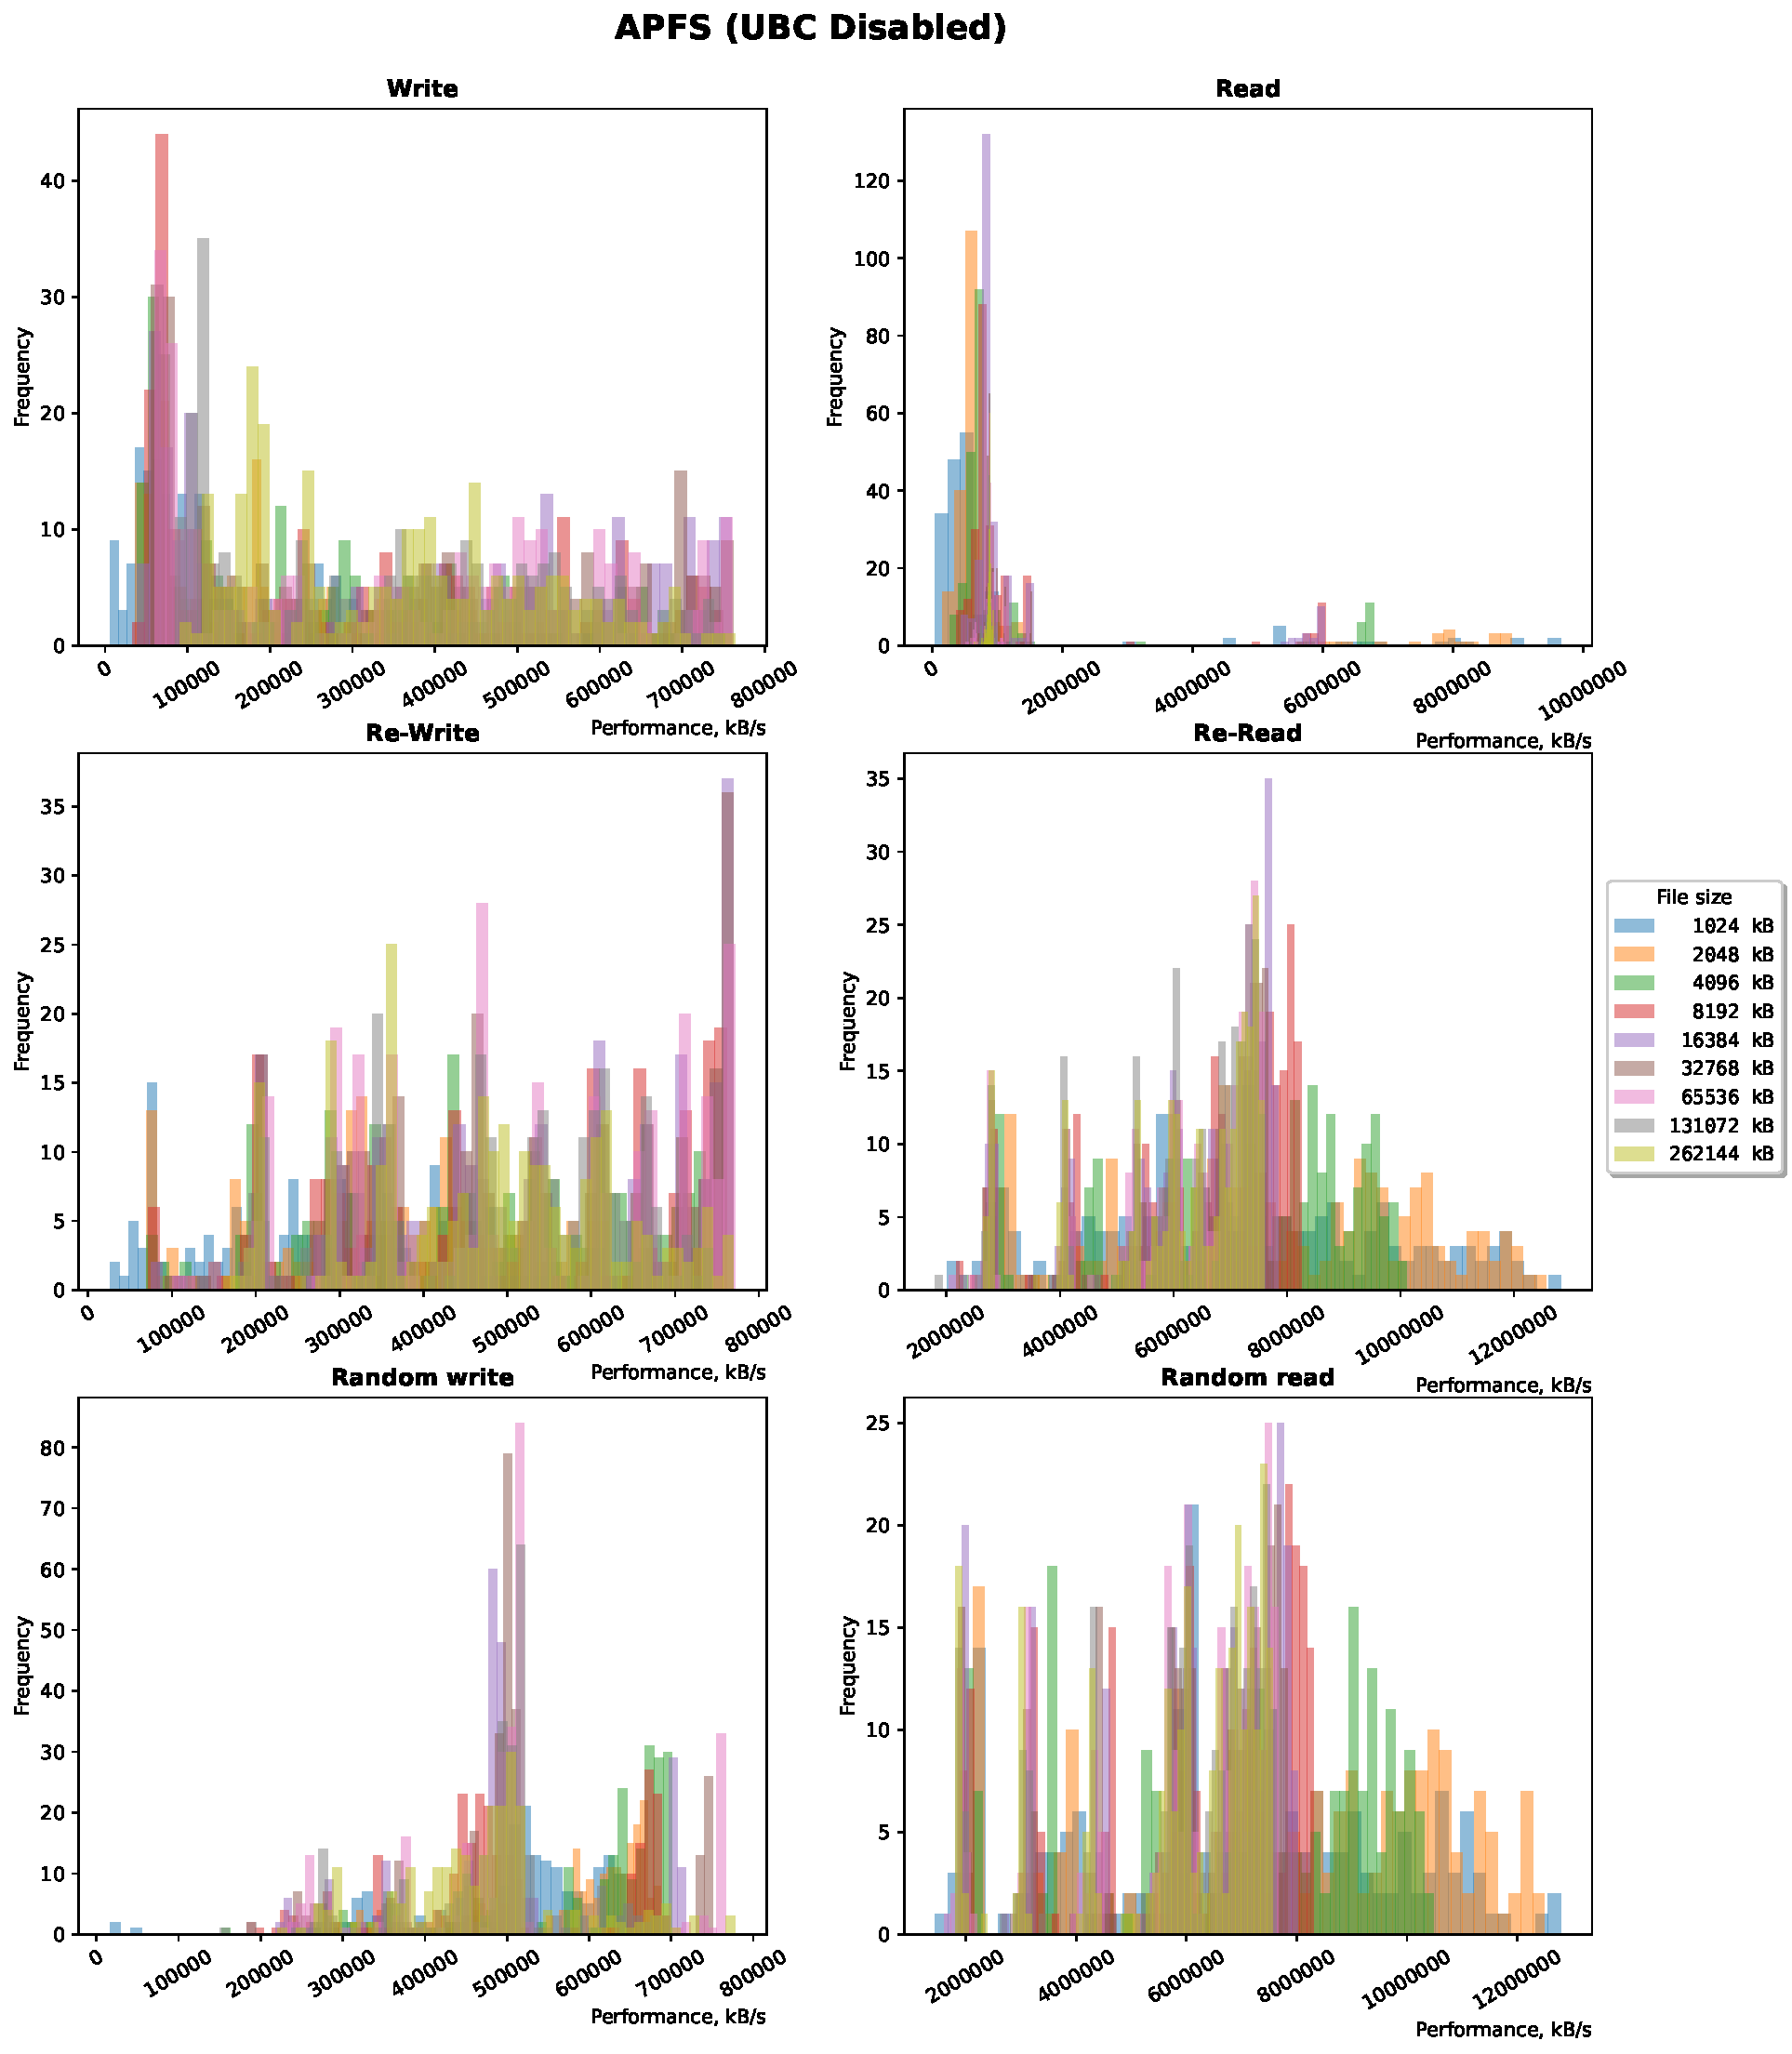
\includegraphics[width=1.0\textwidth]{figures.nosync/benchmarking/APFS/APFS-UBC Disabled-hist.pdf}
	\end{center}
	\caption[Performance comparison for APFS with the UBC disabled]{Performance comparison of different file sizes for APFS with the UBC disabled}
\end{figure}
\clearpage

If we for each filesystem, each state of the \gls{UBC}, and each file operation test consider a function $F(fis, bis)$ be the maximum performance of the 20 data points for a file size $fis$ and buffer size $bis$, we can calculate the joint mean and joint covariance of each $F$ by creating a probability mass function $PMF(x, y)$ which represents the probability that $fis$ is $x$ and $bis$ is y. Table~\ref{tbl:stat-ffs_ubc_enabled} and Table~\ref{tbl:stat-ffs_ubc_disabled} presents the joint mean and joint covariance of \gls{FFS} with the \gls{UBC} enabled and disabled, respectively. Table~\ref{tbl:stat-gcsf_ubc_enabled} and Table~\ref{tbl:stat-gcsf_ubc_disabled} presents the joint mean and joint covariance of \gls{GCSF} with the \gls{UBC} enabled and disabled, respectively. Table~\ref{tbl:stat-fffs_ubc_enabled} and Table~\ref{tbl:stat-fffs_ubc_disabled} presents the joint mean and joint covariance of \gls{FFFS} with the \gls{UBC} enabled and disabled, respectively. Table~\ref{tbl:stat-apfs_ubc_enabled} and Table~\ref{tbl:stat-apfs_ubc_disabled} presents the joint mean and joint covariance of \gls{APFS} with the \gls{UBC} enabled and disabled, respectively. In all these tables, the variance of $fis$ is higher than the variance of $bis$, indicating that higher filesystem performance is more dependant on a big file size than the buffer size. Although, as the variance of $bis$ is also a positive value, it indicates that a bigger buffer size also contributes to a better filesystem performance.


	\begin{table}
	\caption{Joint mean and joint covariance of FFS (UBC Enabled)}
	\begin{tabular}{| c | c | c |}
	\hline
	{} & \textbf{Joint mean} & \textbf{Joint covariance}\\
	\hline
	\textbf{FFS (UBC Enabled)} & {} & {} \\
Write & $\left[ \begin{array}{rr} 46282.58 & 2773.83 \end{array}\right] $ & $\left[ \begin{array}{rr} 5324082245.37 & 38883230.85 \\ 38883230.85 & 17363294.13 \end{array}\right] $\\ 
{} & {} & {} \\
Read & $\left[ \begin{array}{rr} 38673.29 & 1747.55 \end{array}\right] $ & $\left[ \begin{array}{rr} 2600175283.80 & 32445956.69 \\ 32445956.69 & 12322920.65 \end{array}\right] $\\ 
{} & {} & {} \\
Re-Write & $\left[ \begin{array}{rr} 73718.32 & 1896.79 \end{array}\right] $ & $\left[ \begin{array}{rr} 8229485734.06 & 44620204.31 \\ 44620204.31 & 14241380.43 \end{array}\right] $\\ 
{} & {} & {} \\
Re-Read & $\left[ \begin{array}{rr} 69925.03 & 1909.71 \end{array}\right] $ & $\left[ \begin{array}{rr} 7525155884.01 & 37461587.43 \\ 37461587.43 & 14587416.34 \end{array}\right] $\\ 
{} & {} & {} \\
Random write & $\left[ \begin{array}{rr} 82852.93 & 1991.52 \end{array}\right] $ & $\left[ \begin{array}{rr} 8572576873.99 & 42787661.50 \\ 42787661.50 & 15944949.79 \end{array}\right] $\\ 
{} & {} & {} \\
Random read & $\left[ \begin{array}{rr} 68896.02 & 2017.43 \end{array}\right] $ & $\left[ \begin{array}{rr} 7449720363.26 & 40221359.14 \\ 40221359.14 & 15196243.50 \end{array}\right] $\\ 
{} & {} & {} \\

	\hline
	\end{tabular}
	\label{tbl:stat-ffs_ubc_enabled}
	\end{table}

\FloatBarrier

	\begin{table}
	\caption{Joint mean and joint covariance of FFS (UBC Disabled)}
	\begin{tabular}{| c | c | c |}
	\hline
	{} & \textbf{Joint mean} & \textbf{Joint covariance}\\
	\hline
	\textbf{FFS (UBC Disabled)} & {} & {} \\
Write & $\left[ \begin{array}{rr} 49373.26 & 2114.62 \end{array}\right] $ & $\left[ \begin{array}{rr} 2166899348.58 & 22601759.84 \\ 22601759.84 & 17020309.97 \end{array}\right] $\\ 
{} & {} & {} \\
Read & $\left[ \begin{array}{rr} 38222.44 & 2105.72 \end{array}\right] $ & $\left[ \begin{array}{rr} 1945112455.48 & 27816431.75 \\ 27816431.75 & 15987101.57 \end{array}\right] $\\ 
{} & {} & {} \\
Re-Write & $\left[ \begin{array}{rr} 49246.56 & 2041.57 \end{array}\right] $ & $\left[ \begin{array}{rr} 2223646080.34 & 21394476.97 \\ 21394476.97 & 16420986.82 \end{array}\right] $\\ 
{} & {} & {} \\
Re-Read & $\left[ \begin{array}{rr} 37271.94 & 2050.28 \end{array}\right] $ & $\left[ \begin{array}{rr} 1922429155.72 & 28516377.19 \\ 28516377.19 & 15607078.80 \end{array}\right] $\\ 
{} & {} & {} \\
Random write & $\left[ \begin{array}{rr} 49068.83 & 2048.72 \end{array}\right] $ & $\left[ \begin{array}{rr} 2212105854.64 & 21326201.74 \\ 21326201.74 & 16473964.98 \end{array}\right] $\\ 
{} & {} & {} \\
Random read & $\left[ \begin{array}{rr} 19602.82 & 1139.91 \end{array}\right] $ & $\left[ \begin{array}{rr} 1264167991.96 & 24132021.45 \\ 24132021.45 & 7602541.11 \end{array}\right] $\\ 
{} & {} & {} \\

	\hline
	\end{tabular}
	\label{tbl:stat-ffs_ubc_disabled}
	\end{table}

\FloatBarrier



	\begin{table}
	\caption{Joint mean and joint covariance of GCSF (UBC Enabled)}
	\begin{tabular}{| c | c | c |}
	\hline
	{} & \textbf{Joint mean} & \textbf{Joint covariance}\\
	\hline
	\textbf{GCSF (UBC Enabled)} & {} & {} \\
Write & $\left[ \begin{array}{rr} 54647.03 & 2400.27 \end{array}\right] $ & $\left[ \begin{array}{rr} 2251861738.51 & 12174208.85 \\ 12174208.85 & 19499499.91 \end{array}\right] $\\ 
{} & {} & {} \\
Read & $\left[ \begin{array}{rr} 22046.15 & 1641.46 \end{array}\right] $ & $\left[ \begin{array}{rr} 977346154.88 & 13126458.96 \\ 13126458.96 & 11829218.19 \end{array}\right] $\\ 
{} & {} & {} \\
Re-Write & $\left[ \begin{array}{rr} 53132.30 & 2337.76 \end{array}\right] $ & $\left[ \begin{array}{rr} 2280624142.80 & 16296801.40 \\ 16296801.40 & 18856697.26 \end{array}\right] $\\ 
{} & {} & {} \\
Re-Read & $\left[ \begin{array}{rr} 37018.77 & 1752.82 \end{array}\right] $ & $\left[ \begin{array}{rr} 1870121324.37 & 21217869.17 \\ 21217869.17 & 12998670.08 \end{array}\right] $\\ 
{} & {} & {} \\
Random write & $\left[ \begin{array}{rr} 52381.62 & 2035.99 \end{array}\right] $ & $\left[ \begin{array}{rr} 2215217719.90 & 17268192.34 \\ 17268192.34 & 16650919.80 \end{array}\right] $\\ 
{} & {} & {} \\
Random read & $\left[ \begin{array}{rr} 36437.73 & 1829.68 \end{array}\right] $ & $\left[ \begin{array}{rr} 1848921543.25 & 22614156.98 \\ 22614156.98 & 13351147.54 \end{array}\right] $\\ 
{} & {} & {} \\

	\hline
	\end{tabular}
	\label{tbl:stat-gcsf_ubc_enabled}
	\end{table}

\FloatBarrier

	\begin{table}
	\caption{Joint mean and joint covariance of GCSF (UBC Disabled)}
	\begin{tabular}{| c | c | c |}
	\hline
	{} & \textbf{Joint mean} & \textbf{Joint covariance}\\
	\hline
	\textbf{GCSF (UBC Disabled)} & {} & {} \\
Write & $\left[ \begin{array}{rr} 48093.41 & 2089.56 \end{array}\right] $ & $\left[ \begin{array}{rr} 2113904153.26 & 18979810.38 \\ 18979810.38 & 16792968.48 \end{array}\right] $\\ 
{} & {} & {} \\
Read & $\left[ \begin{array}{rr} 37280.36 & 2110.41 \end{array}\right] $ & $\left[ \begin{array}{rr} 1815613473.62 & 31309295.20 \\ 31309295.20 & 13392527.66 \end{array}\right] $\\ 
{} & {} & {} \\
Re-Write & $\left[ \begin{array}{rr} 48462.87 & 2107.10 \end{array}\right] $ & $\left[ \begin{array}{rr} 2164949562.66 & 19521321.26 \\ 19521321.26 & 16914995.70 \end{array}\right] $\\ 
{} & {} & {} \\
Re-Read & $\left[ \begin{array}{rr} 36446.66 & 2133.02 \end{array}\right] $ & $\left[ \begin{array}{rr} 1883567157.35 & 28974865.64 \\ 28974865.64 & 13791810.36 \end{array}\right] $\\ 
{} & {} & {} \\
Random write & $\left[ \begin{array}{rr} 49870.39 & 1865.25 \end{array}\right] $ & $\left[ \begin{array}{rr} 2186002094.46 & 14947526.86 \\ 14947526.86 & 15288804.93 \end{array}\right] $\\ 
{} & {} & {} \\
Random read & $\left[ \begin{array}{rr} 36421.57 & 2183.24 \end{array}\right] $ & $\left[ \begin{array}{rr} 1904233213.15 & 27534818.98 \\ 27534818.98 & 14234459.33 \end{array}\right] $\\ 
{} & {} & {} \\

	\hline
	\end{tabular}
	\label{tbl:stat-gcsf_ubc_disabled}
	\end{table}

\FloatBarrier



	\begin{table}
	\caption{Joint mean and joint covariance of FFFS (UBC Enabled)}
	\begin{tabular}{| c | c | c |}
	\hline
	{} & \textbf{Joint mean} & \textbf{Joint covariance}\\
	\hline
	\textbf{FFFS (UBC Enabled)} & {} & {} \\
Write & $\left[ \begin{array}{rr} 68947.50 & 1951.14 \end{array}\right] $ & $\left[ \begin{array}{rr} 7436792834.74 & 39645552.64 \\ 39645552.64 & 15671811.85 \end{array}\right] $\\ 
{} & {} & {} \\
Read & $\left[ \begin{array}{rr} 37449.89 & 1871.20 \end{array}\right] $ & $\left[ \begin{array}{rr} 1914457655.95 & 22764249.95 \\ 22764249.95 & 14043875.41 \end{array}\right] $\\ 
{} & {} & {} \\
Re-Write & $\left[ \begin{array}{rr} 67464.03 & 1919.32 \end{array}\right] $ & $\left[ \begin{array}{rr} 7366373842.82 & 40257204.39 \\ 40257204.39 & 15389501.34 \end{array}\right] $\\ 
{} & {} & {} \\
Re-Read & $\left[ \begin{array}{rr} 70009.69 & 1906.95 \end{array}\right] $ & $\left[ \begin{array}{rr} 7665975042.67 & 35839816.45 \\ 35839816.45 & 14442682.04 \end{array}\right] $\\ 
{} & {} & {} \\
Random write & $\left[ \begin{array}{rr} 67365.42 & 1915.15 \end{array}\right] $ & $\left[ \begin{array}{rr} 7362043491.97 & 40367179.54 \\ 40367179.54 & 15351646.71 \end{array}\right] $\\ 
{} & {} & {} \\
Random read & $\left[ \begin{array}{rr} 69237.43 & 2018.64 \end{array}\right] $ & $\left[ \begin{array}{rr} 7605233191.03 & 38624832.17 \\ 38624832.17 & 15109239.14 \end{array}\right] $\\ 
{} & {} & {} \\

	\hline
	\end{tabular}
	\label{tbl:stat-fffs_ubc_enabled}
	\end{table}

\FloatBarrier

	\begin{table}
	\caption{Joint mean and joint covariance of FFFS (UBC Disabled)}
	\begin{tabular}{| c | c | c |}
	\hline
	{} & \textbf{Joint mean} & \textbf{Joint covariance}\\
	\hline
	\textbf{FFFS (UBC Disabled)} & {} & {} \\
Write & $\left[ \begin{array}{rr} 69152.27 & 1956.50 \end{array}\right] $ & $\left[ \begin{array}{rr} 7448036812.87 & 39852267.48 \\ 39852267.48 & 15719710.90 \end{array}\right] $\\ 
{} & {} & {} \\
Read & $\left[ \begin{array}{rr} 67858.44 & 2167.22 \end{array}\right] $ & $\left[ \begin{array}{rr} 7405881404.34 & 43603875.16 \\ 43603875.16 & 16758971.52 \end{array}\right] $\\ 
{} & {} & {} \\
Re-Write & $\left[ \begin{array}{rr} 67476.02 & 1920.32 \end{array}\right] $ & $\left[ \begin{array}{rr} 7363116033.56 & 40534174.12 \\ 40534174.12 & 15406184.55 \end{array}\right] $\\ 
{} & {} & {} \\
Re-Read & $\left[ \begin{array}{rr} 66213.91 & 2123.31 \end{array}\right] $ & $\left[ \begin{array}{rr} 7290497366.67 & 44044197.30 \\ 44044197.30 & 16448082.52 \end{array}\right] $\\ 
{} & {} & {} \\
Random write & $\left[ \begin{array}{rr} 66604.83 & 1906.58 \end{array}\right] $ & $\left[ \begin{array}{rr} 7312485557.20 & 41063701.96 \\ 41063701.96 & 15275024.61 \end{array}\right] $\\ 
{} & {} & {} \\
Random read & $\left[ \begin{array}{rr} 57993.96 & 1816.08 \end{array}\right] $ & $\left[ \begin{array}{rr} 6770964006.13 & 45310923.12 \\ 45310923.12 & 14139624.33 \end{array}\right] $\\ 
{} & {} & {} \\

	\hline
	\end{tabular}
	\label{tbl:stat-fffs_ubc_disabled}
	\end{table}

\FloatBarrier



	\begin{table}
	\caption{Joint mean and joint covariance of APFS (UBC Enabled)}
	\begin{tabular}{| c | c | c |}
	\hline
	{} & \textbf{Joint mean} & \textbf{Joint covariance}\\
	\hline
	\textbf{APFS (UBC Enabled)} & {} & {} \\
Write & $\left[ \begin{array}{rr} 55146.35 & 2022.43 \end{array}\right] $ & $\left[ \begin{array}{rr} 6373209287.15 & 45720332.46 \\ 45720332.46 & 15337800.11 \end{array}\right] $\\ 
{} & {} & {} \\
Read & $\left[ \begin{array}{rr} 65590.59 & 1872.16 \end{array}\right] $ & $\left[ \begin{array}{rr} 7233582970.81 & 38515007.19 \\ 38515007.19 & 13992645.66 \end{array}\right] $\\ 
{} & {} & {} \\
Re-Write & $\left[ \begin{array}{rr} 46182.55 & 1572.60 \end{array}\right] $ & $\left[ \begin{array}{rr} 5730706585.82 & 47145687.50 \\ 47145687.50 & 11847293.04 \end{array}\right] $\\ 
{} & {} & {} \\
Re-Read & $\left[ \begin{array}{rr} 62249.84 & 1801.30 \end{array}\right] $ & $\left[ \begin{array}{rr} 7028991755.50 & 39431229.41 \\ 39431229.41 & 13340049.04 \end{array}\right] $\\ 
{} & {} & {} \\
Random write & $\left[ \begin{array}{rr} 38643.77 & 1451.66 \end{array}\right] $ & $\left[ \begin{array}{rr} 4954634427.36 & 49115633.14 \\ 49115633.14 & 10597363.49 \end{array}\right] $\\ 
{} & {} & {} \\
Random read & $\left[ \begin{array}{rr} 61200.10 & 1895.03 \end{array}\right] $ & $\left[ \begin{array}{rr} 6947430246.19 & 41990504.87 \\ 41990504.87 & 13842639.11 \end{array}\right] $\\ 
{} & {} & {} \\

	\hline
	\end{tabular}
	\label{tbl:stat-apfs_ubc_enabled}
	\end{table}

\FloatBarrier

	\begin{table}
	\caption{Joint mean and joint covariance of APFS (UBC Disabled)}
	\begin{tabular}{| c | c | c |}
	\hline
	{} & \textbf{Joint mean} & \textbf{Joint covariance}\\
	\hline
	\hline
Write & $\left[ \begin{array}{rr} 74496.24 & 3449.96 \end{array}\right] $ & $\left[ \begin{array}{rr} 7833121694.94 & 49307668.52 \\ 49307668.52 & 23841549.94 \end{array}\right] $\\ 
{} & {} & {} \\ 
Read & $\left[ \begin{array}{rr} 50064.88 & 3043.59 \end{array}\right] $ & $\left[ \begin{array}{rr} 6022459844.96 & -5901443.95 \\ -5901443.95 & 22170364.18 \end{array}\right] $\\ 
{} & {} & {} \\ 
Re-Write & $\left[ \begin{array}{rr} 66685.54 & 2627.95 \end{array}\right] $ & $\left[ \begin{array}{rr} 7313451449.66 & 53636275.69 \\ 53636275.69 & 19593921.72 \end{array}\right] $\\ 
{} & {} & {} \\ 
Re-Read & $\left[ \begin{array}{rr} 56691.24 & 1694.72 \end{array}\right] $ & $\left[ \begin{array}{rr} 6684776973.38 & 44020640.65 \\ 44020640.65 & 12536573.40 \end{array}\right] $\\ 
{} & {} & {} \\ 
Random write & $\left[ \begin{array}{rr} 60414.93 & 2285.97 \end{array}\right] $ & $\left[ \begin{array}{rr} 6968437399.85 & 62133530.14 \\ 62133530.14 & 18565489.45 \end{array}\right] $\\ 
{} & {} & {} \\ 
Random read & $\left[ \begin{array}{rr} 56092.28 & 1787.26 \end{array}\right] $ & $\left[ \begin{array}{rr} 6613967187.30 & 46549432.14 \\ 46549432.14 & 13021007.73 \end{array}\right] $\\ 
{} & {} & {} \\ 

	\hline
	\end{tabular}
	\label{tbl:stat-apfs_ubc_disabled}
	\end{table}

\FloatBarrier

As none of the filesystem benchmarks show a well-defined distribution, such as a normal distribution or a exponential distribution, confidence intervals of the data can instead be calculated using bootstrapping. Bootstrapped confidence intervals using 20 bootstrap replicates with a confidence level of 80\% are presented in the tables below. \Cref{tbl:bootstrap-table-ffs,tbl:bootstrap-table-gcsf,tbl:bootstrap-table-fffs,tbl:bootstrap-table-apfs} presents the bootstrapped confidence intervals of \gls{FFS}, \gls{GCSF}, \gls{FFFS}, and \gls{APFS}, respectively.
\FloatBarrier

	\begin{table}
	\caption{80\% confidence intervals of the different benchmark test performances of FFS}
	\begin{tabular}{| c | c | c |}
	\hline
	{} & \textbf{UBC enabled} & \textbf{UBC disabled} \\
	\hline
	\hline
	Write &$\left[ \begin{array}{rr} 383.41 & 2377.39 \end{array}\right] $ &$\left[ \begin{array}{rr} 641.67 & 1574.03 \end{array}\right] $\\ 
Read &$\left[ \begin{array}{rr} 1341270.67 & 7538272.93 \end{array}\right] $ &$\left[ \begin{array}{rr} 47169.84 & 83878.36 \end{array}\right] $\\ 
Re-Write &$\left[ \begin{array}{rr} 270.04 & 2080.96 \end{array}\right] $ &$\left[ \begin{array}{rr} 362.08 & 1096.02 \end{array}\right] $\\ 
Re-Read &$\left[ \begin{array}{rr} 3849025.53 & 8006988.37 \end{array}\right] $ &$\left[ \begin{array}{rr} 42082.91 & 80268.79 \end{array}\right] $\\ 
Random write &$\left[ \begin{array}{rr} 700.32 & 2140.88 \end{array}\right] $ &$\left[ \begin{array}{rr} 523.66 & 1183.84 \end{array}\right] $\\ 
Random read &$\left[ \begin{array}{rr} 3473267.87 & 8090937.63 \end{array}\right] $ &$\left[ \begin{array}{rr} 3745.02 & 35606.68 \end{array}\right] $\\ 

		\hline
		\end{tabular}
		\label{tbl:bootstrap-table-ffs}
		\end{table}
	

	\begin{table}[ht!]
	\caption{80\% confidence intervals of the different benchmark test performances of GCSF}
	\begin{tabular}{| c | c | c |}
	\hline
	{} & \textbf{UBC enabled} & \textbf{UBC disabled} \\
	\hline
	\hline
	Write &$\left[ \begin{array}{rr} 240.06 & 2808.04 \end{array}\right] $ &$\left[ \begin{array}{rr} 428.27 & 2350.23 \end{array}\right] $\\ 
Read &$\left[ \begin{array}{rr} 222884.66 & 5778790.84 \end{array}\right] $ &$\left[ \begin{array}{rr} 488346.79 & 2280029.81 \end{array}\right] $\\ 
Re-Write &$\left[ \begin{array}{rr} 731.29 & 2360.41 \end{array}\right] $ &$\left[ \begin{array}{rr} 371.39 & 1961.11 \end{array}\right] $\\ 
Re-Read &$\left[ \begin{array}{rr} 3690780.53 & 7878976.87 \end{array}\right] $ &$\left[ \begin{array}{rr} 102391.85 & 2174746.05 \end{array}\right] $\\ 
Random write &$\left[ \begin{array}{rr} 379.20 & 3374.20 \end{array}\right] $ &$\left[ \begin{array}{rr} 427.72 & 2350.98 \end{array}\right] $\\ 
Random read &$\left[ \begin{array}{rr} 3505422.83 & 7262968.07 \end{array}\right] $ &$\left[ \begin{array}{rr} 118359.05 & 2181830.25 \end{array}\right] $\\ 

		\hline
		\end{tabular}
		\label{tbl:bootstrap-table-gcsf}
		\end{table}
	

	\begin{table}[ht!]
	\caption{80\% confidence intervals of the different benchmark test performances of FFFS}
	\begin{tabular}{| c | c | c |}
	\hline
	{} & \textbf{UBC enabled} & \textbf{UBC disabled} \\
	\hline
	\hline
	Write &$\left[ \begin{array}{rr} 5575.49 & 8901.11 \end{array}\right] $ &$\left[ \begin{array}{rr} 6652.68 & 9106.82 \end{array}\right] $\\ 
Read &$\left[ \begin{array}{rr} 2747489.83 & 7953376.07 \end{array}\right] $ &$\left[ \begin{array}{rr} 45695.20 & 92160.20 \end{array}\right] $\\ 
Re-Write &$\left[ \begin{array}{rr} 6043.06 & 7461.54 \end{array}\right] $ &$\left[ \begin{array}{rr} 5793.10 & 7358.10 \end{array}\right] $\\ 
Re-Read &$\left[ \begin{array}{rr} 3346179.80 & 8726841.30 \end{array}\right] $ &$\left[ \begin{array}{rr} 51593.83 & 89506.77 \end{array}\right] $\\ 
Random write &$\left[ \begin{array}{rr} 5679.60 & 7125.30 \end{array}\right] $ &$\left[ \begin{array}{rr} 6139.73 & 7342.77 \end{array}\right] $\\ 
Random read &$\left[ \begin{array}{rr} 3175468.27 & 8427944.33 \end{array}\right] $ &$\left[ \begin{array}{rr} 20296.83 & 32727.47 \end{array}\right] $\\ 

		\hline
		\end{tabular}
		\label{tbl:bootstrap-table-fffs}
		\end{table}
	

	\begin{table}[ht!]
	\caption{80\% confidence intervals of the different benchmark test performances of APFS}
	\begin{tabular}{| c | c | c |}
	\hline
	{} & \textbf{UBC enabled} & \textbf{UBC disabled} \\
	\hline
	\hline
	Write &$\left[ \begin{array}{rr} 162517.11 & 838770.49 \end{array}\right] $ &$\left[ \begin{array}{rr} 35991.41 & 691115.79 \end{array}\right] $\\ 
Read &$\left[ \begin{array}{rr} 4569677.13 & 9695911.97 \end{array}\right] $ &$\left[ \begin{array}{rr} 349215.85 & 1641614.55 \end{array}\right] $\\ 
Re-Write &$\left[ \begin{array}{rr} 254092.41 & 1532373.19 \end{array}\right] $ &$\left[ \begin{array}{rr} 191324.31 & 687133.09 \end{array}\right] $\\ 
Re-Read &$\left[ \begin{array}{rr} 6132939.99 & 10053118.21 \end{array}\right] $ &$\left[ \begin{array}{rr} 4005136.05 & 8986816.75 \end{array}\right] $\\ 
Random write &$\left[ \begin{array}{rr} 389294.62 & 1237453.58 \end{array}\right] $ &$\left[ \begin{array}{rr} 291738.23 & 634012.97 \end{array}\right] $\\ 
Random read &$\left[ \begin{array}{rr} 5044277.32 & 10173507.88 \end{array}\right] $ &$\left[ \begin{array}{rr} 4721144.02 & 9020239.58 \end{array}\right] $\\ 

		\hline
		\end{tabular}
		\label{tbl:bootstrap-table-apfs}
		\end{table}
	

% Plotting a scatter plot of the performance for each test per filesystem, we can visualize the distribution of values dependant on the buffer size and file size, using one axis the buffer size and the color of the scatter points as the file size. \Cref{fig:bench_ffs_ubc_scatter_read,fig:bench_ffs_ubc_scatter_write,fig:bench_ffs_ubc_scatter_re-read,fig:bench_ffs_ubc_scatter_re-write,fig:bench_ffs_ubc_scatter_rnd_read,fig:bench_ffs_ubc_scatter_rnd_write} presents a scatter plot for the Write, Read, Re-Write, Re-Read, Random Write and Random Read tests for \gls{FFS} with the \gls{UBC} enabled, respectively. \Cref{fig:bench_ffs_no_ubc_scatter_read,fig:bench_ffs_no_ubc_scatter_write,fig:bench_ffs_no_ubc_scatter_re-read,fig:bench_ffs_no_ubc_scatter_re-write,fig:bench_ffs_no_ubc_scatter_rnd_read,fig:bench_ffs_no_ubc_scatter_rnd_write} presents a scatter plot for the Write, Read, Re-Write, Re-Read, Random Write and Random Read tests for \gls{FFS} with the \gls{UBC} disabled, respectively. We can see that, for both states of the \gls{UBC}, the three read tests follow a normal distribution curve with increasing performance for the first buffer sizes, and decreasing performance after a maximum around the \SI[per-mode = symbol]{512}{\kilo\byte} buffer size. The write tests follow a constant performance distribution where the performance does not change significantly between buffer sizes. Different file sizes have different performances (increased file size generally increases the performance, as we know since previous arguments) but there is no major improvement for bigger buffer sizes, as opposed to the read tests.

% \Cref{fig:bench_gcsf_ubc_scatter_read,fig:bench_gcsf_ubc_scatter_write,fig:bench_gcsf_ubc_scatter_re-read,fig:bench_gcsf_ubc_scatter_re-write,fig:bench_gcsf_ubc_scatter_rnd_read,fig:bench_gcsf_ubc_scatter_rnd_write} presents a scatter plot for the Write, Read, Re-Write, Re-Read, Random Write and Random Read tests for \gls{GCSF} with the \gls{UBC} enabled, respectively. \Cref{fig:bench_gcsf_no_ubc_scatter_read,fig:bench_gcsf_no_ubc_scatter_write,fig:bench_gcsf_no_ubc_scatter_re-read,fig:bench_gcsf_no_ubc_scatter_re-write,fig:bench_gcsf_no_ubc_scatter_rnd_read,fig:bench_gcsf_no_ubc_scatter_rnd_write} presents a scatter plot for the Write, Read, Re-Write, Re-Read, Random Write and Random Read tests for \gls{GCSF} with the \gls{UBC} disabled, respectively. 

% \Cref{fig:bench_fffs_ubc_scatter_read,fig:bench_fffs_ubc_scatter_write,fig:bench_fffs_ubc_scatter_re-read,fig:bench_fffs_ubc_scatter_re-write,fig:bench_fffs_ubc_scatter_rnd_read,fig:bench_fffs_ubc_scatter_rnd_write} presents a scatter plot for the Write, Read, Re-Write, Re-Read, Random Write and Random Read tests for \gls{FFFS} with the \gls{UBC} enabled, respectively. \Cref{fig:bench_fffs_no_ubc_scatter_read,fig:bench_fffs_no_ubc_scatter_write,fig:bench_fffs_no_ubc_scatter_re-read,fig:bench_fffs_no_ubc_scatter_re-write,fig:bench_fffs_no_ubc_scatter_rnd_read,fig:bench_fffs_no_ubc_scatter_rnd_write} presents a scatter plot for the Write, Read, Re-Write, Re-Read, Random Write and Random Read tests for \gls{FFFS} with the \gls{UBC} disabled, respectively. 

% \Cref{fig:bench_apfs_ubc_scatter_read,fig:bench_apfs_ubc_scatter_write,fig:bench_apfs_ubc_scatter_re-read,fig:bench_apfs_ubc_scatter_re-write,fig:bench_apfs_ubc_scatter_rnd_read,fig:bench_apfs_ubc_scatter_rnd_write} presents a scatter plot for the Write, Read, Re-Write, Re-Read, Random Write and Random Read tests for \gls{APFS} with the \gls{UBC} enabled, respectively. \Cref{fig:bench_apfs_no_ubc_scatter_read,fig:bench_apfs_no_ubc_scatter_write,fig:bench_apfs_no_ubc_scatter_re-read,fig:bench_apfs_no_ubc_scatter_re-write,fig:bench_apfs_no_ubc_scatter_rnd_read,fig:bench_apfs_no_ubc_scatter_rnd_write} presents a scatter plot for the Write, Read, Re-Write, Re-Read, Random Write and Random Read tests for \gls{APFS} with the \gls{UBC} disabled, respectively.

% % FFS
% \clearpage
% \begin{figure}[!htb]
% 	\label{fig:bench_ffs_ubc_scatter_read}
% 	\begin{center}
% 		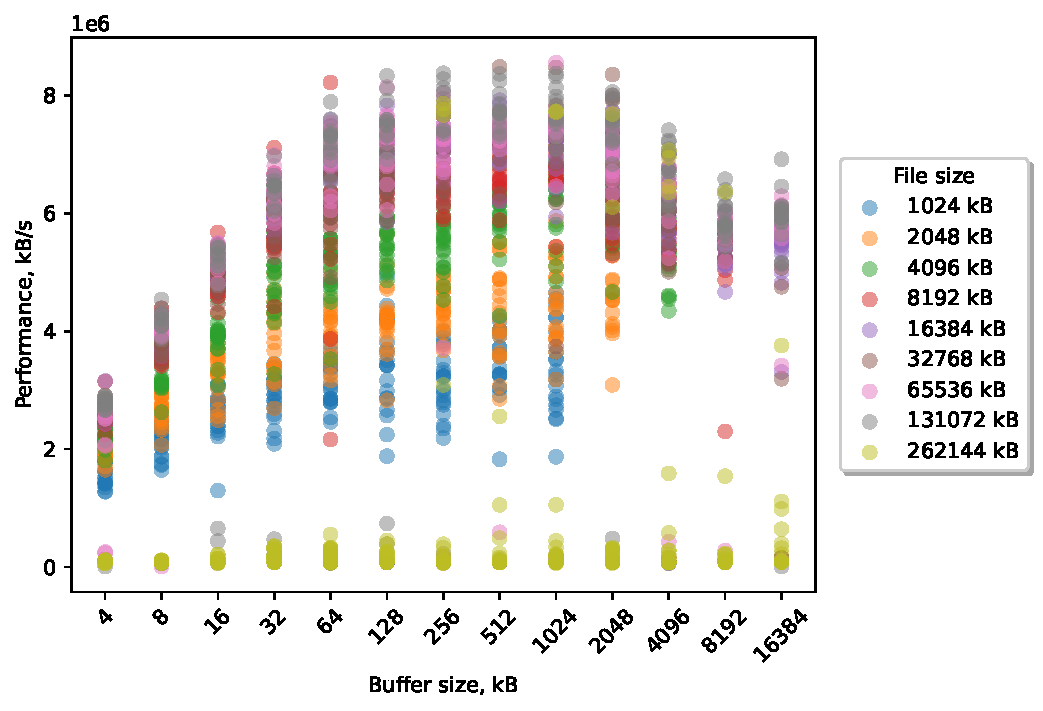
\includegraphics[width=0.8\textwidth]{figures.nosync/benchmarking/FFS/scatter-UBC Enabled-Read.pdf}
% 	\end{center}
% 	\caption[Comparison of Read performance for file size and buffer size for FFS with the UBC enabled]{Performance comparison of different file sizes and buffer sizes for FFS Read with the UBC enabled}
% \end{figure}
% \begin{figure}[!htb]
% 	\label{fig:bench_ffs_ubc_scatter_write}
% 	\begin{center}
% 		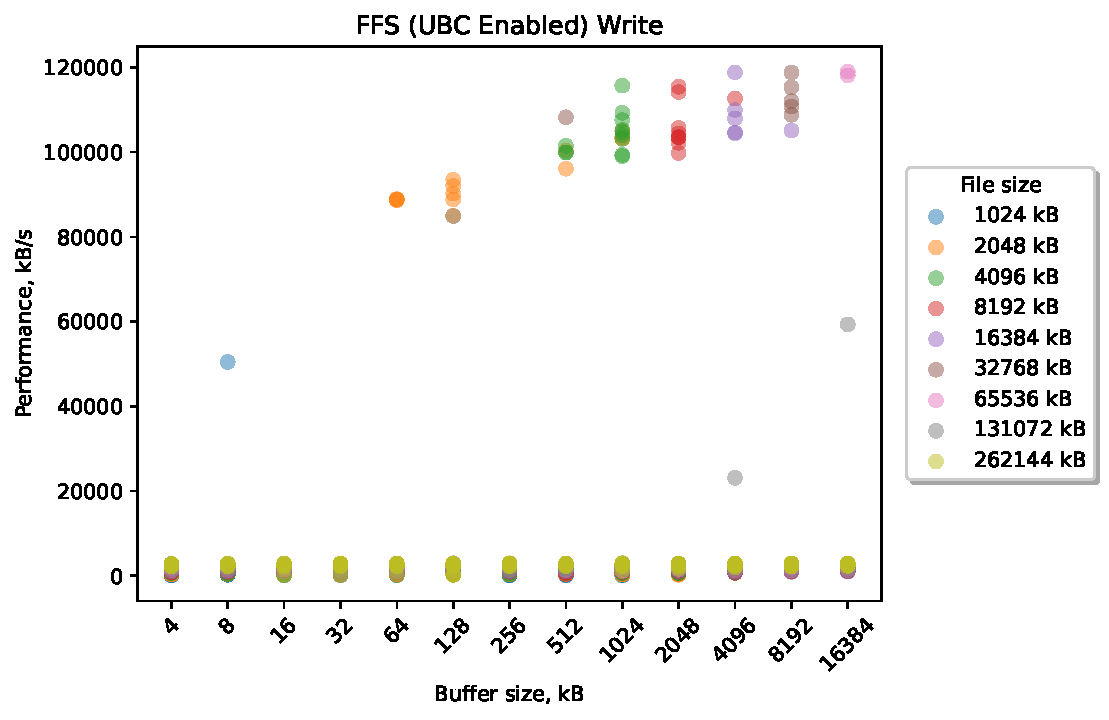
\includegraphics[width=0.8\textwidth]{figures.nosync/benchmarking/FFS/scatter-UBC Enabled-Write.pdf}
% 	\end{center}
% 	\caption[Comparison of Write performance for file size and buffer size for FFS with the UBC enabled]{Performance comparison of different file sizes and buffer sizes for FFS Write with the UBC enabled}
% \end{figure}
% \clearpage
% \begin{figure}[!htb]
% 	\label{fig:bench_ffs_ubc_scatter_re-read}
% 	\begin{center}
% 		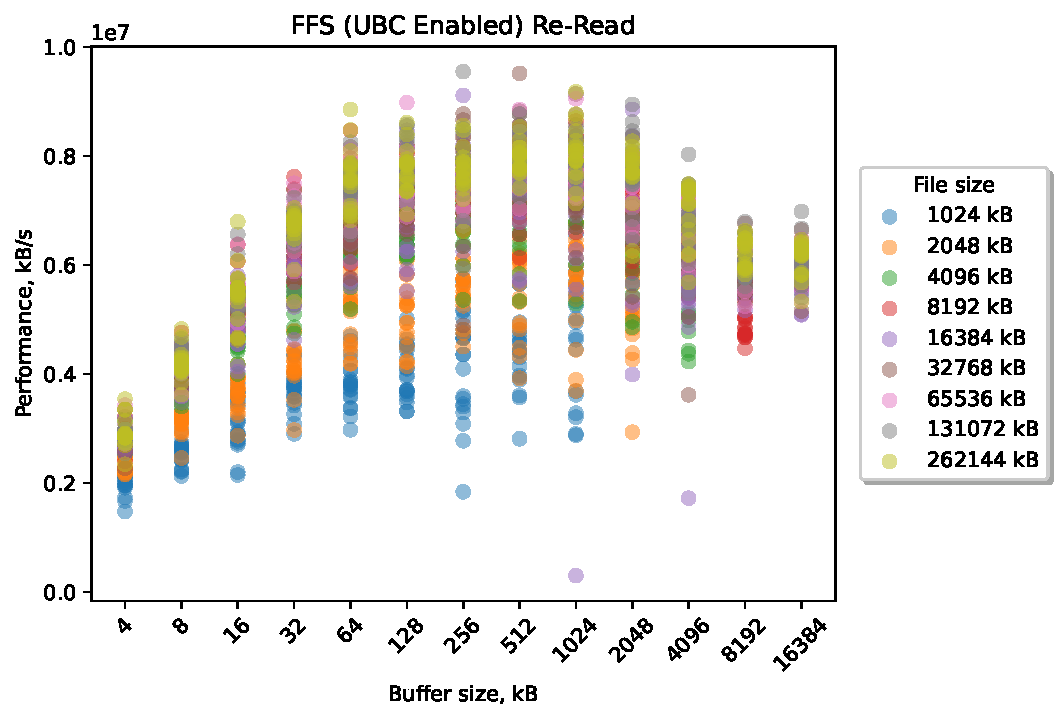
\includegraphics[width=0.8\textwidth]{figures.nosync/benchmarking/FFS/scatter-UBC Enabled-Re-Read.pdf}
% 	\end{center}
% 	\caption[Comparison of Re-Read performance for file size and buffer size for FFS with the UBC enabled]{Performance comparison of different file sizes and buffer sizes for FFS Re-Read with the UBC enabled}
% \end{figure}
% \begin{figure}[!htb]
% 	\label{fig:bench_ffs_ubc_scatter_re-write}
% 	\begin{center}
% 		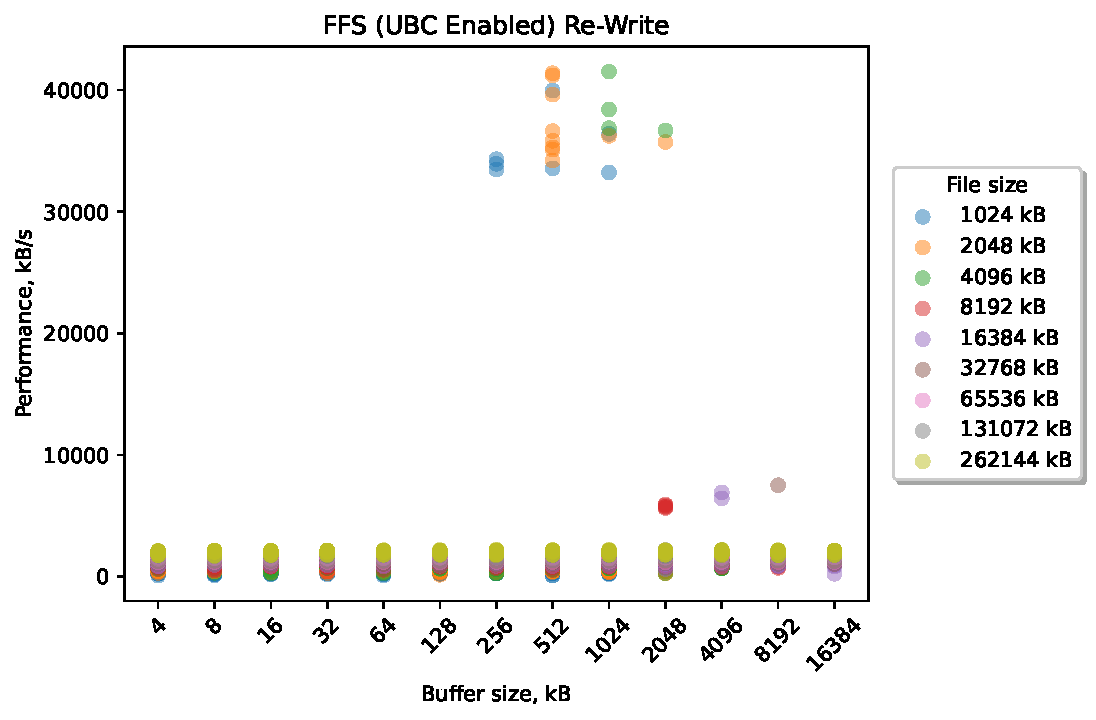
\includegraphics[width=0.8\textwidth]{figures.nosync/benchmarking/FFS/scatter-UBC Enabled-Re-Write.pdf}
% 	\end{center}
% 	\caption[Comparison of Re-Write performance for file size and buffer size for FFS with the UBC enabled]{Performance comparison of different file sizes and buffer sizes for FFS Re-Write with the UBC enabled}
% \end{figure}
% \clearpage
% \begin{figure}[!htb]
% 	\label{fig:bench_ffs_ubc_scatter_rnd_read}
% 	\begin{center}
% 		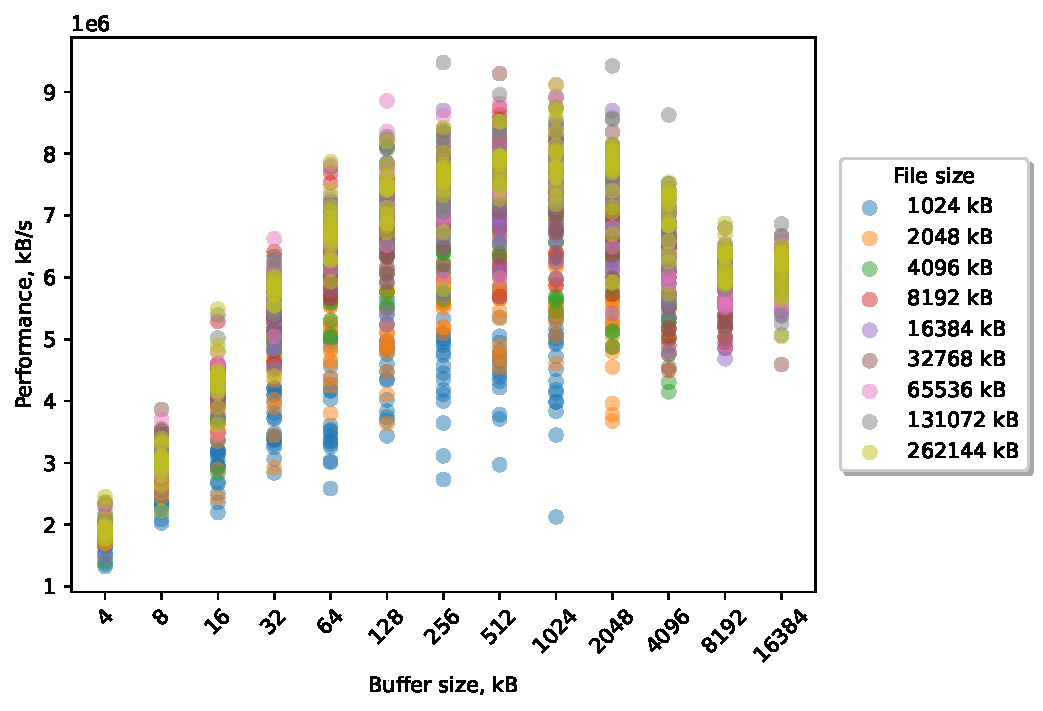
\includegraphics[width=0.8\textwidth]{figures.nosync/benchmarking/FFS/scatter-UBC Enabled-Random read.pdf}
% 	\end{center}
% 	\caption[Comparison of Random Read performance for file size and buffer size for FFS with the UBC enabled]{Performance comparison of different file sizes and buffer sizes for FFS Random Read with the UBC enabled}
% \end{figure}
% \begin{figure}[!htb]
% 	\label{fig:bench_ffs_ubc_scatter_rnd_write}
% 	\begin{center}
% 		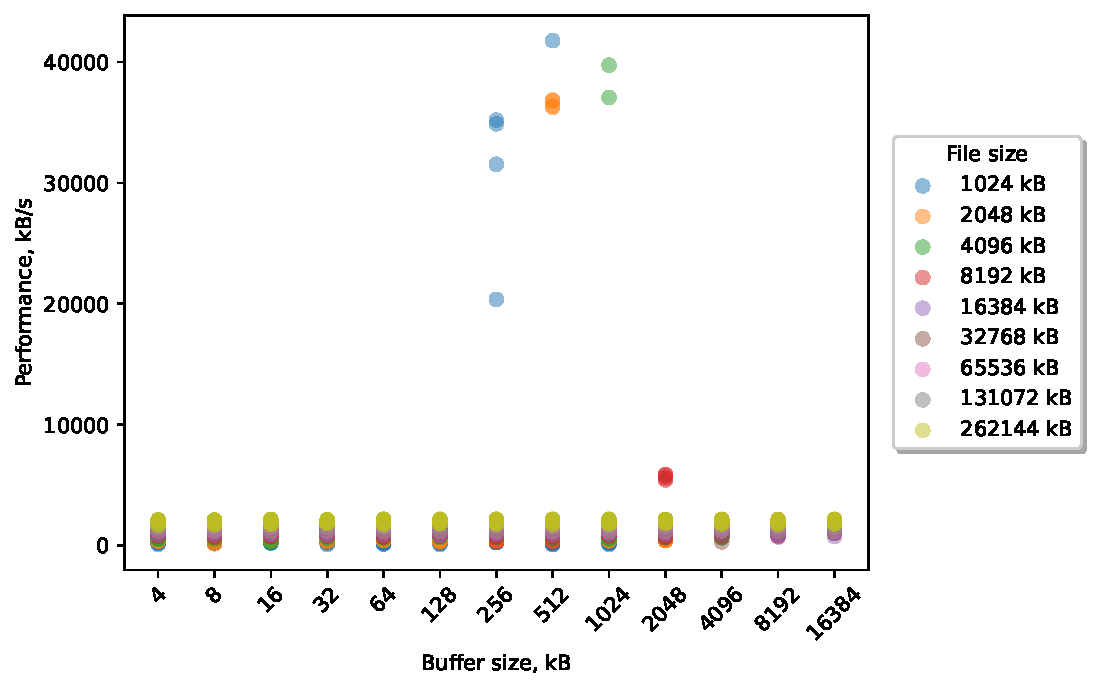
\includegraphics[width=0.8\textwidth]{figures.nosync/benchmarking/FFS/scatter-UBC Enabled-Random write.pdf}
% 	\end{center}
% 	\caption[Comparison of Random Write performance for file size and buffer size for FFS with the UBC enabled]{Performance comparison of different file sizes and buffer sizes for FFS Random Write with the UBC enabled}
% \end{figure}
% \clearpage

% \begin{figure}[!htb]
% 	\label{fig:bench_ffs_no_ubc_scatter_read}
% 	\begin{center}
% 		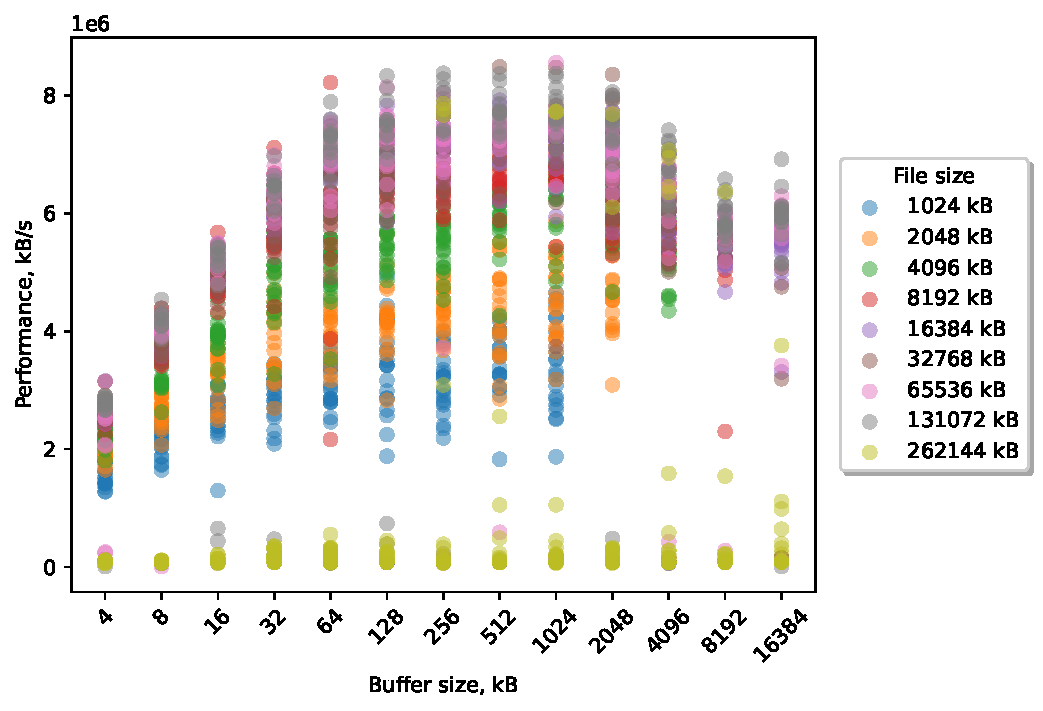
\includegraphics[width=0.8\textwidth]{figures.nosync/benchmarking/FFS/scatter-UBC Enabled-Read.pdf}
% 	\end{center}
% 	\caption[Comparison of Read performance for file size and buffer size for FFS with the UBC disabled]{Performance comparison of different file sizes and buffer sizes for FFS Read with the UBC enabled}
% \end{figure}
% \begin{figure}[!htb]
% 	\label{fig:bench_ffs_no_ubc_scatter_write}
% 	\begin{center}
% 		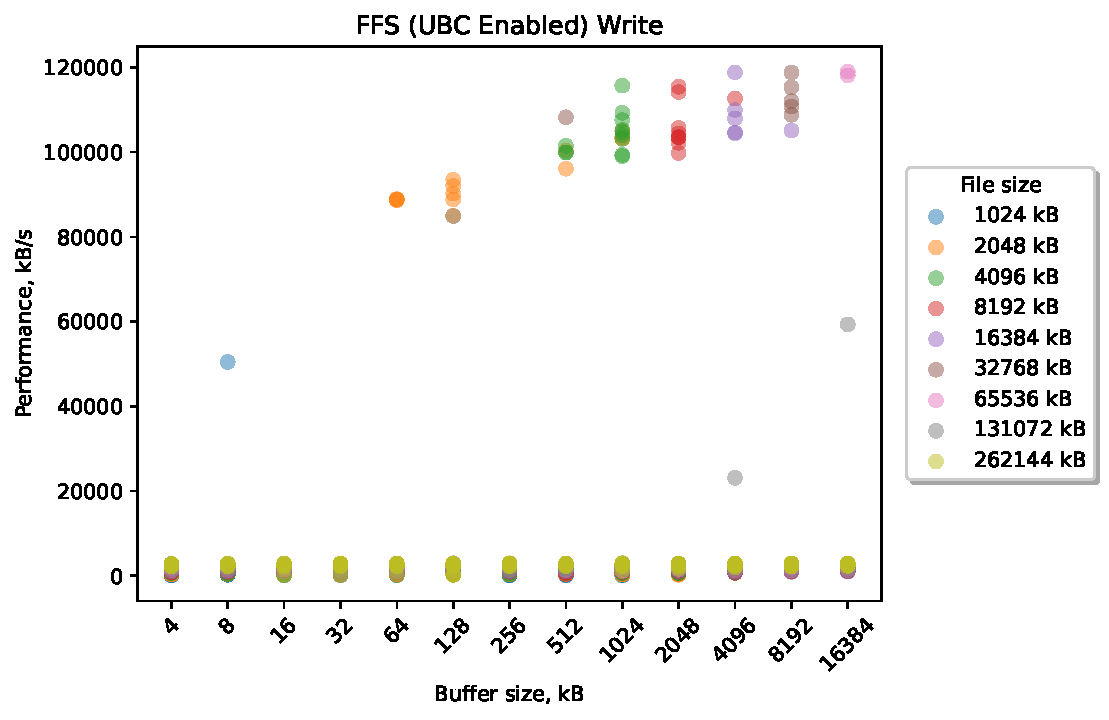
\includegraphics[width=0.8\textwidth]{figures.nosync/benchmarking/FFS/scatter-UBC Enabled-Write.pdf}
% 	\end{center}
% 	\caption[Comparison of Write performance for file size and buffer size for FFS with the UBC disabled]{Performance comparison of different file sizes and buffer sizes for FFS Write with the UBC enabled}
% \end{figure}
% \clearpage
% \begin{figure}[!htb]
% 	\label{fig:bench_ffs_no_ubc_scatter_re-read}
% 	\begin{center}
% 		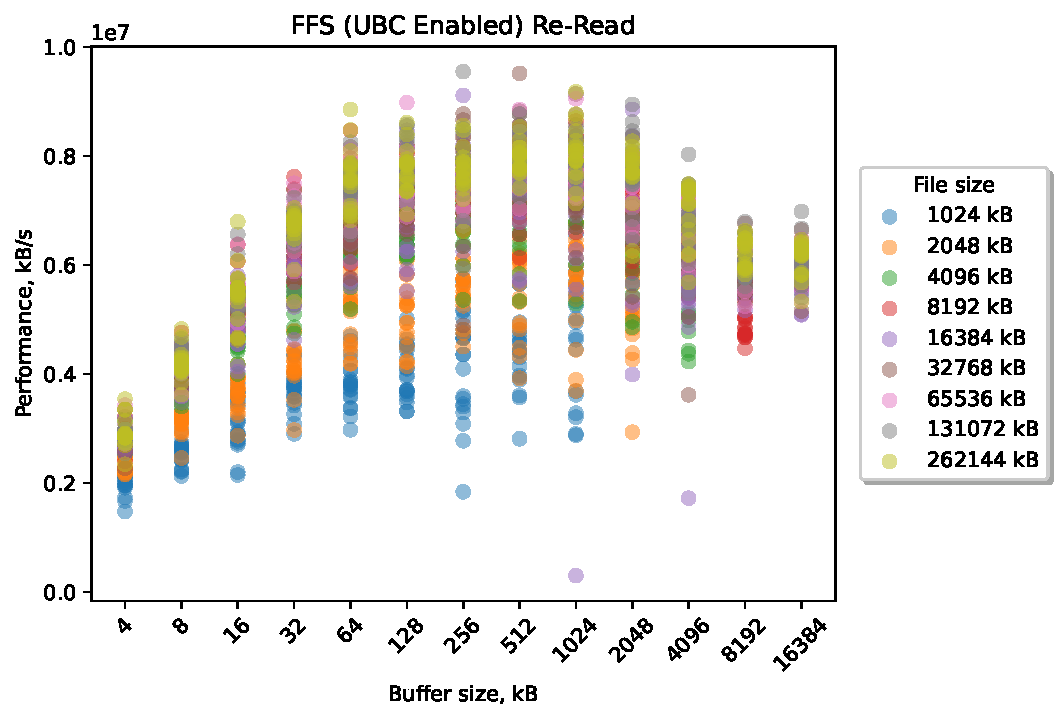
\includegraphics[width=0.8\textwidth]{figures.nosync/benchmarking/FFS/scatter-UBC Enabled-Re-Read.pdf}
% 	\end{center}
% 	\caption[Comparison of Re-Read performance for file size and buffer size for FFS with the UBC disabled]{Performance comparison of different file sizes and buffer sizes for FFS Re-Read with the UBC enabled}
% \end{figure}
% \begin{figure}[!htb]
% 	\label{fig:bench_ffs_no_ubc_scatter_re-write}
% 	\begin{center}
% 		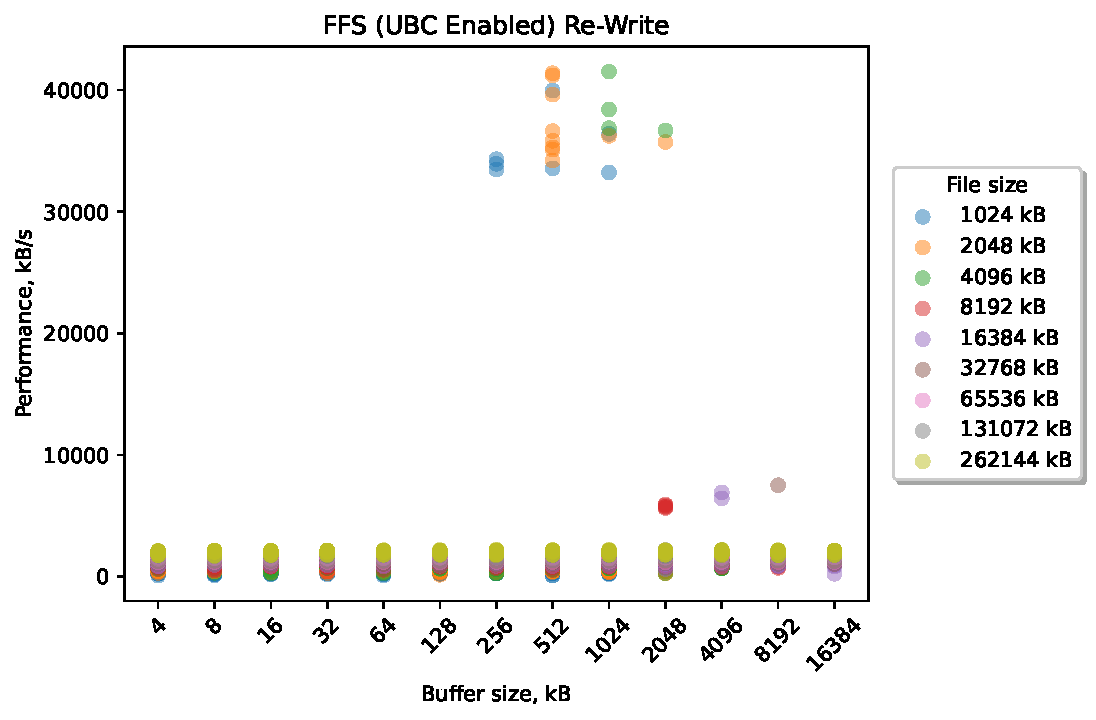
\includegraphics[width=0.8\textwidth]{figures.nosync/benchmarking/FFS/scatter-UBC Enabled-Re-Write.pdf}
% 	\end{center}
% 	\caption[Comparison of Re-Write performance for file size and buffer size for FFS with the UBC disabled]{Performance comparison of different file sizes and buffer sizes for FFS Re-Write with the UBC enabled}
% \end{figure}
% \clearpage
% \begin{figure}[!htb]
% 	\label{fig:bench_ffs_no_ubc_scatter_rnd_read}
% 	\begin{center}
% 		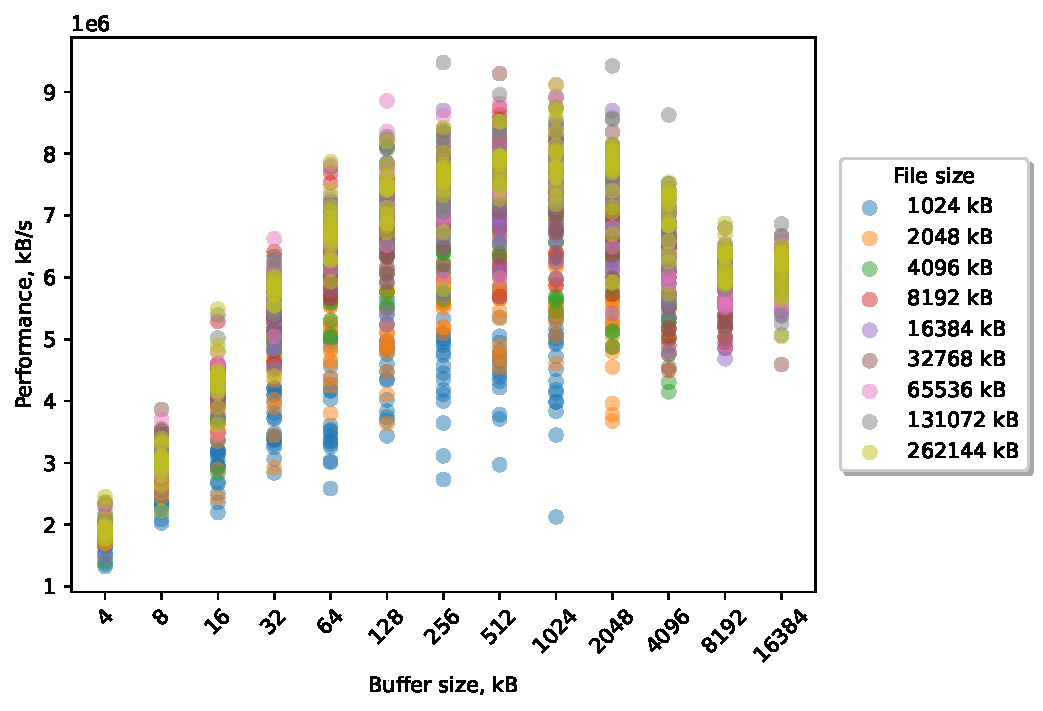
\includegraphics[width=0.8\textwidth]{figures.nosync/benchmarking/FFS/scatter-UBC Enabled-Random read.pdf}
% 	\end{center}
% 	\caption[Comparison of Random Read performance for file size and buffer size for FFS with the UBC disabled]{Performance comparison of different file sizes and buffer sizes for FFS Random Read with the UBC enabled}
% \end{figure}
% \begin{figure}[!htb]
% 	\label{fig:bench_ffs_no_ubc_scatter_rnd_write}
% 	\begin{center}
% 		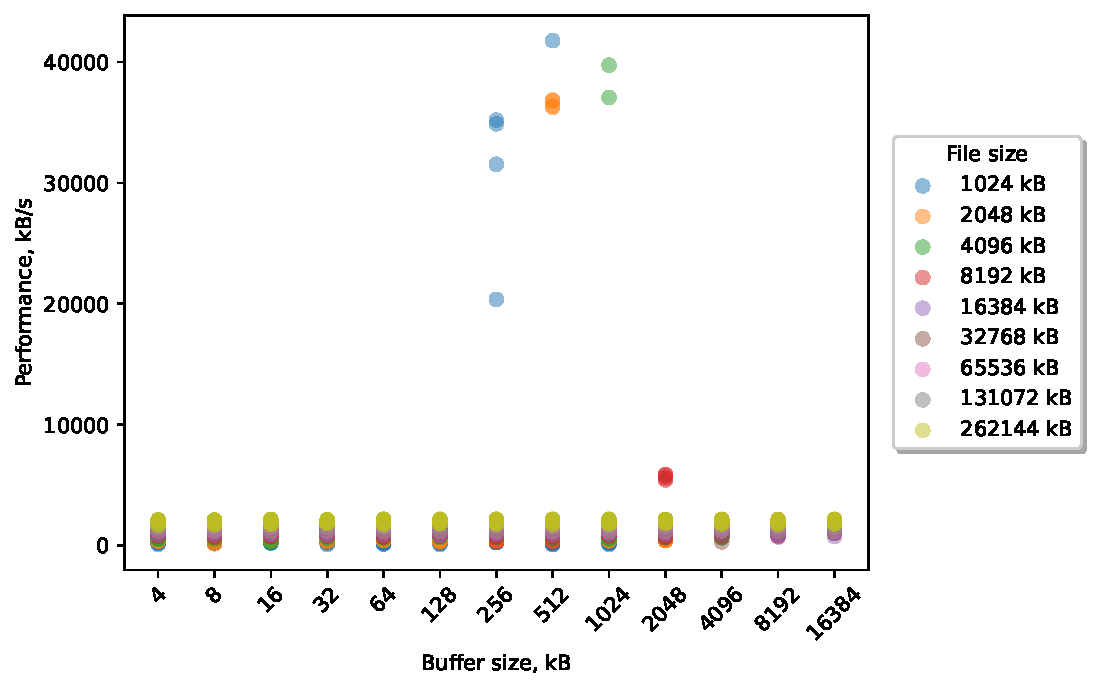
\includegraphics[width=0.8\textwidth]{figures.nosync/benchmarking/FFS/scatter-UBC Enabled-Random write.pdf}
% 	\end{center}
% 	\caption[Comparison of Random Write performance for file size and buffer size for FFS with the UBC disabled]{Performance comparison of different file sizes and buffer sizes for FFS Random Write with the UBC enabled}
% \end{figure}
% \clearpage

% % GCSF

% \begin{figure}[!htb]
% 	\label{fig:bench_gcsf_ubc_scatter_read}
% 	\begin{center}
% 		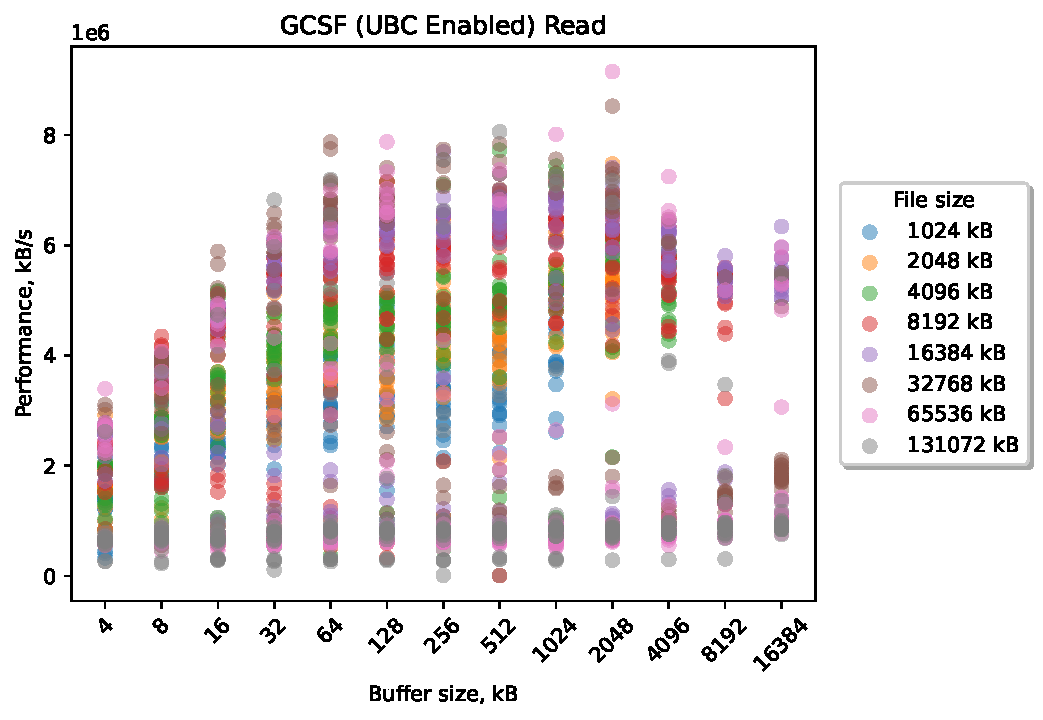
\includegraphics[width=0.8\textwidth]{figures.nosync/benchmarking/GCSF/scatter-UBC Enabled-Read.pdf}
% 	\end{center}
% 	\caption[Comparison of Read performance for file size and buffer size for GCSF with the UBC enabled]{Performance comparison of different file sizes and buffer sizes for GCSF Read with the UBC enabled}
% \end{figure}
% \begin{figure}[!htb]
% 	\label{fig:bench_gcsf_ubc_scatter_write}
% 	\begin{center}
% 		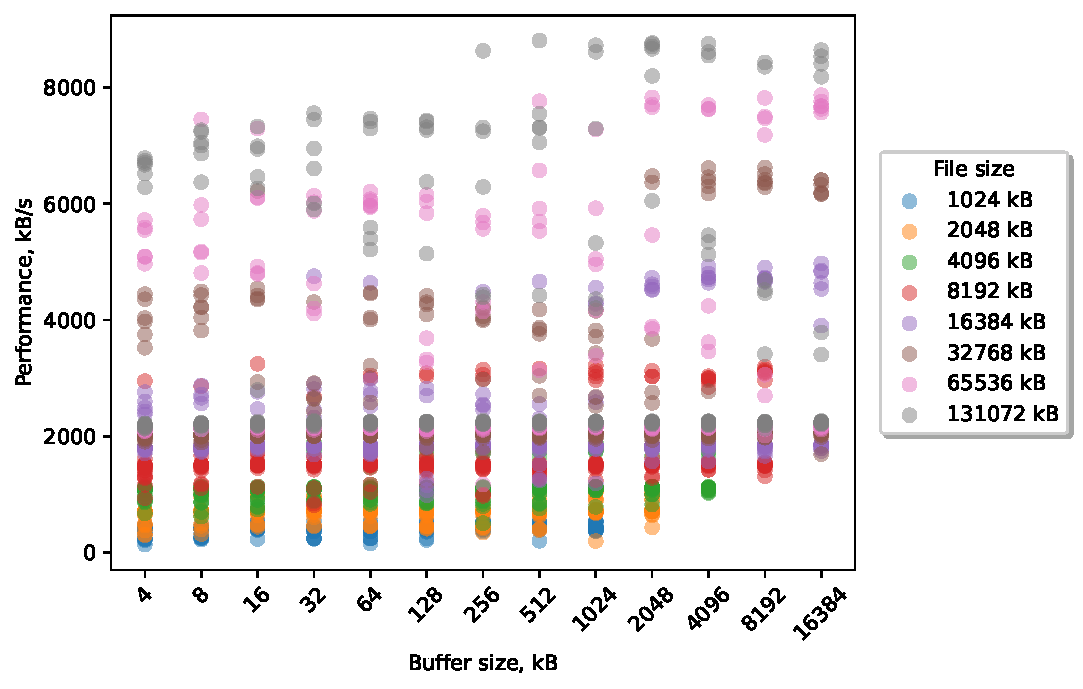
\includegraphics[width=0.8\textwidth]{figures.nosync/benchmarking/GCSF/scatter-UBC Enabled-Write.pdf}
% 	\end{center}
% 	\caption[Comparison of Write performance for file size and buffer size for GCSF with the UBC enabled]{Performance comparison of different file sizes and buffer sizes for GCSF Write with the UBC enabled}
% \end{figure}
% \clearpage
% \begin{figure}[!htb]
% 	\label{fig:bench_gcsf_ubc_scatter_re-read}
% 	\begin{center}
% 		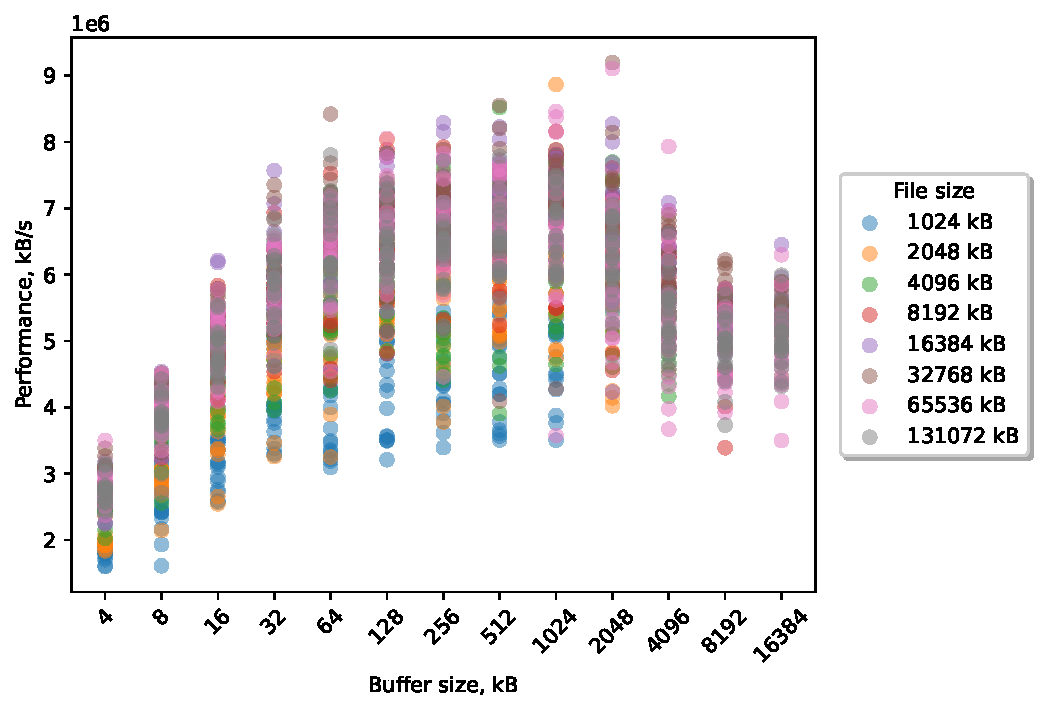
\includegraphics[width=0.8\textwidth]{figures.nosync/benchmarking/GCSF/scatter-UBC Enabled-Re-Read.pdf}
% 	\end{center}
% 	\caption[Comparison of Re-Read performance for file size and buffer size for GCSF with the UBC enabled]{Performance comparison of different file sizes and buffer sizes for GCSF Re-Read with the UBC enabled}
% \end{figure}
% \begin{figure}[!htb]
% 	\label{fig:bench_gcsf_ubc_scatter_re-write}
% 	\begin{center}
% 		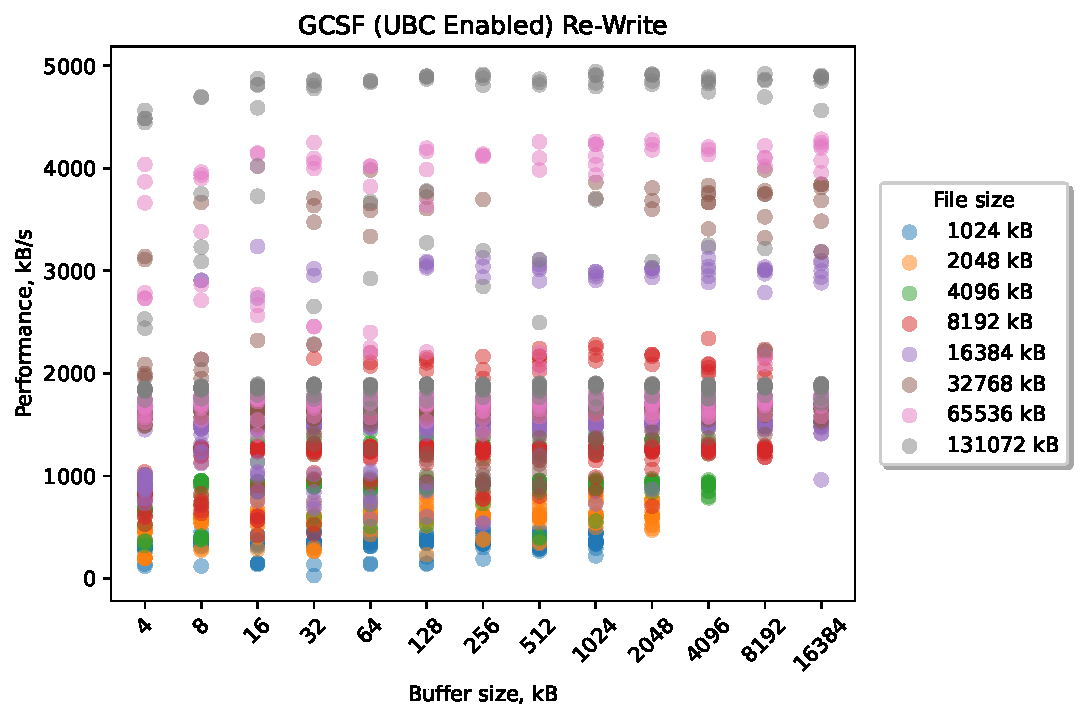
\includegraphics[width=0.8\textwidth]{figures.nosync/benchmarking/GCSF/scatter-UBC Enabled-Re-Write.pdf}
% 	\end{center}
% 	\caption[Comparison of Re-Write performance for file size and buffer size for GCSF with the UBC enabled]{Performance comparison of different file sizes and buffer sizes for GCSF Re-Write with the UBC enabled}
% \end{figure}
% \clearpage
% \begin{figure}[!htb]
% 	\label{fig:bench_gcsf_ubc_scatter_rnd_read}
% 	\begin{center}
% 		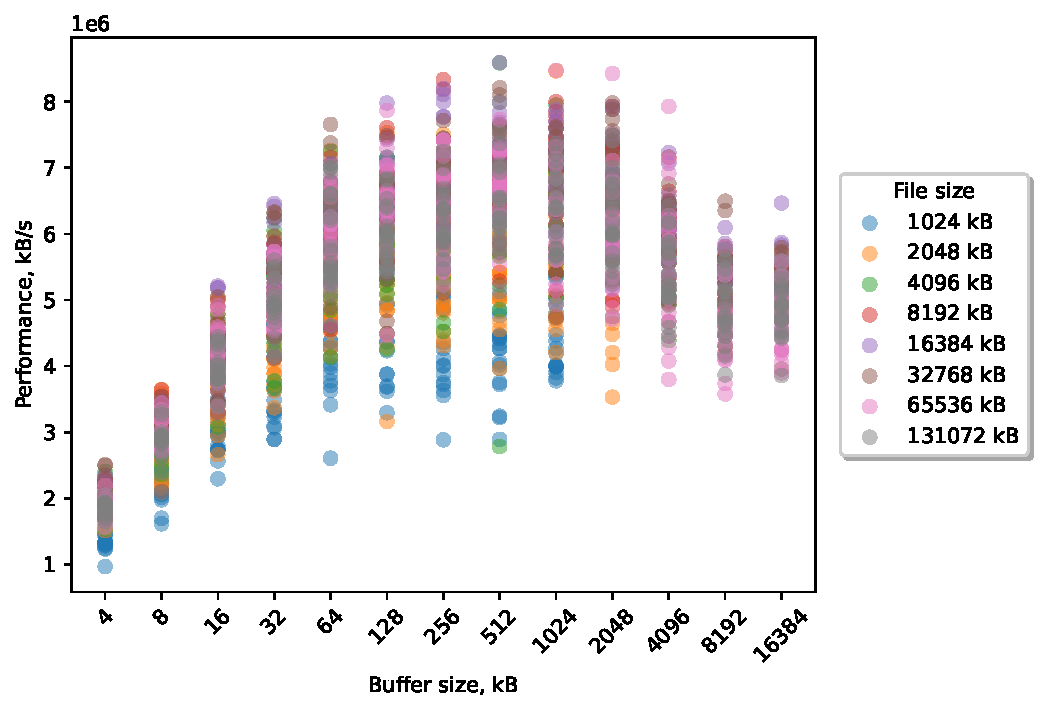
\includegraphics[width=0.8\textwidth]{figures.nosync/benchmarking/GCSF/scatter-UBC Enabled-Random read.pdf}
% 	\end{center}
% 	\caption[Comparison of Random Read performance for file size and buffer size for GCSF with the UBC enabled]{Performance comparison of different file sizes and buffer sizes for GCSF Random Read with the UBC enabled}
% \end{figure}
% \begin{figure}[!htb]
% 	\label{fig:bench_gcsf_ubc_scatter_rnd_write}
% 	\begin{center}
% 		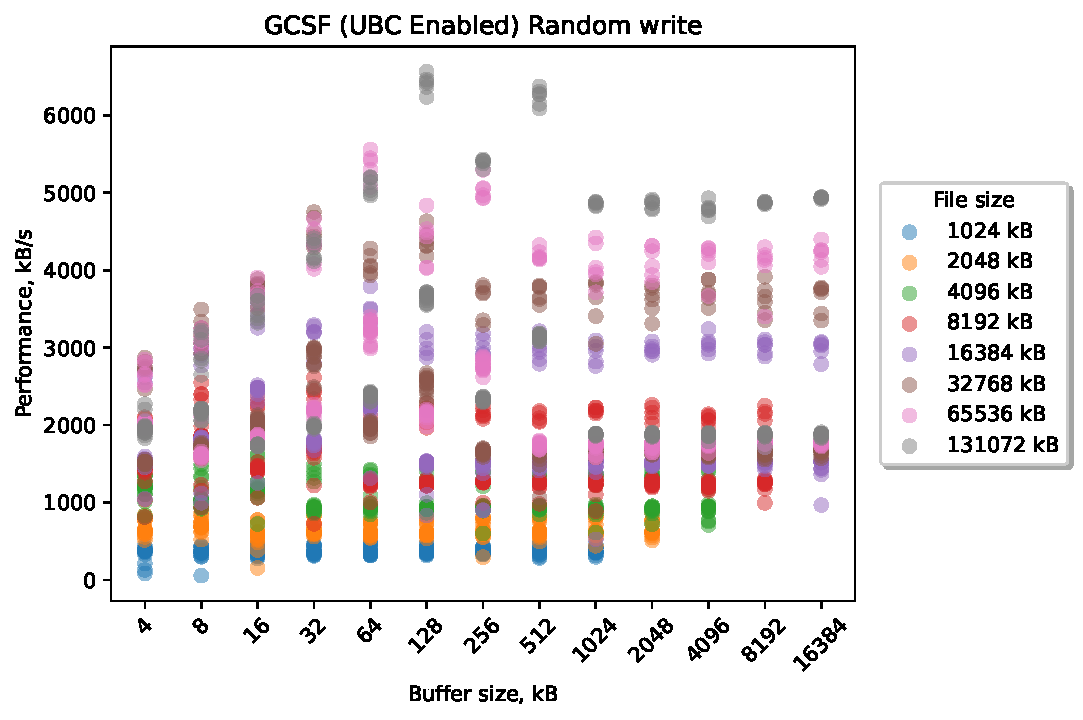
\includegraphics[width=0.8\textwidth]{figures.nosync/benchmarking/GCSF/scatter-UBC Enabled-Random write.pdf}
% 	\end{center}
% 	\caption[Comparison of Random Write performance for file size and buffer size for GCSF with the UBC enabled]{Performance comparison of different file sizes and buffer sizes for GCSF Random Write with the UBC enabled}
% \end{figure}
% \clearpage

% \begin{figure}[!htb]
% 	\label{fig:bench_gcsf_no_ubc_scatter_read}
% 	\begin{center}
% 		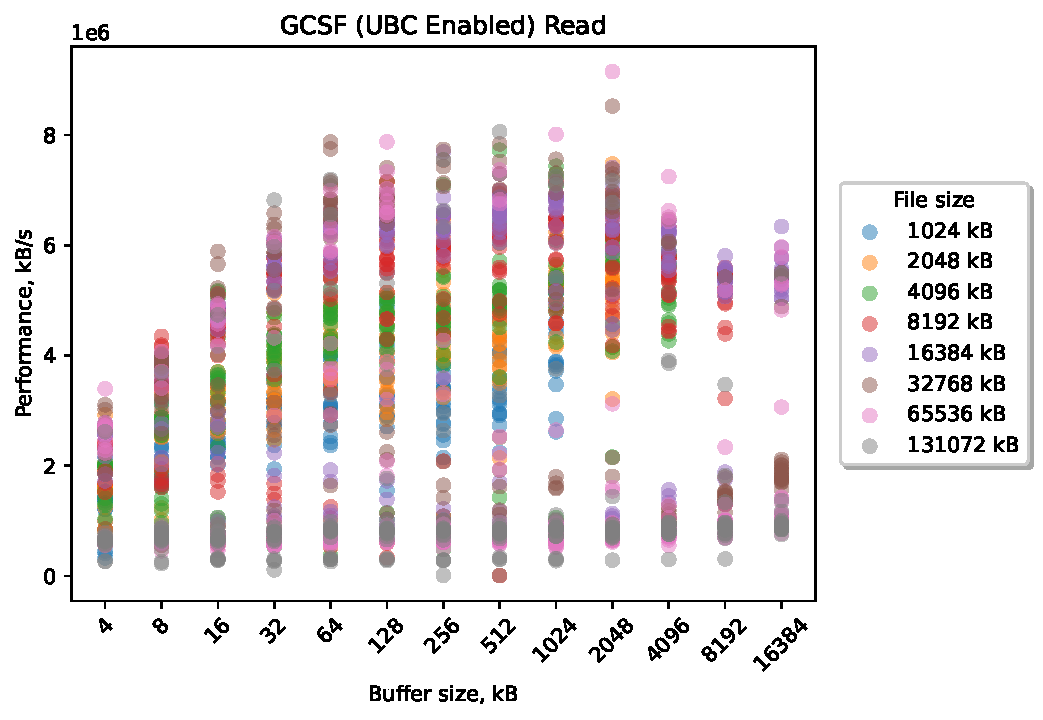
\includegraphics[width=0.8\textwidth]{figures.nosync/benchmarking/GCSF/scatter-UBC Enabled-Read.pdf}
% 	\end{center}
% 	\caption[Comparison of Read performance for file size and buffer size for GCSF with the UBC disabled]{Performance comparison of different file sizes and buffer sizes for GCSF Read with the UBC enabled}
% \end{figure}
% \begin{figure}[!htb]
% 	\label{fig:bench_gcsf_no_ubc_scatter_write}
% 	\begin{center}
% 		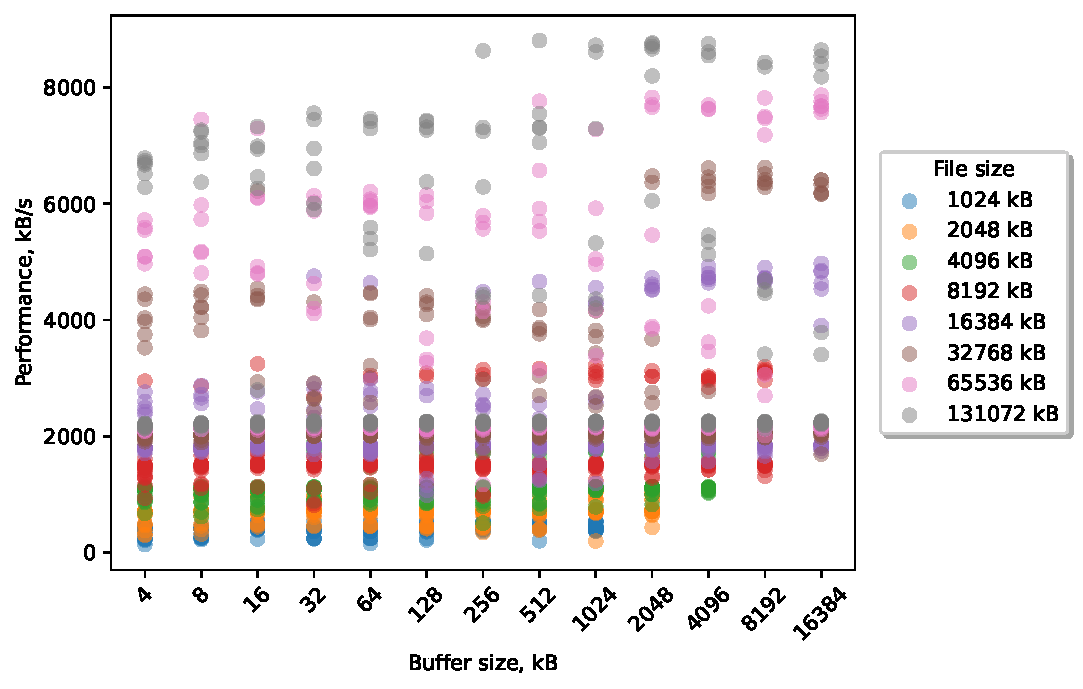
\includegraphics[width=0.8\textwidth]{figures.nosync/benchmarking/GCSF/scatter-UBC Enabled-Write.pdf}
% 	\end{center}
% 	\caption[Comparison of Write performance for file size and buffer size for GCSF with the UBC disabled]{Performance comparison of different file sizes and buffer sizes for GCSF Write with the UBC enabled}
% \end{figure}
% \clearpage
% \begin{figure}[!htb]
% 	\label{fig:bench_gcsf_no_ubc_scatter_re-read}
% 	\begin{center}
% 		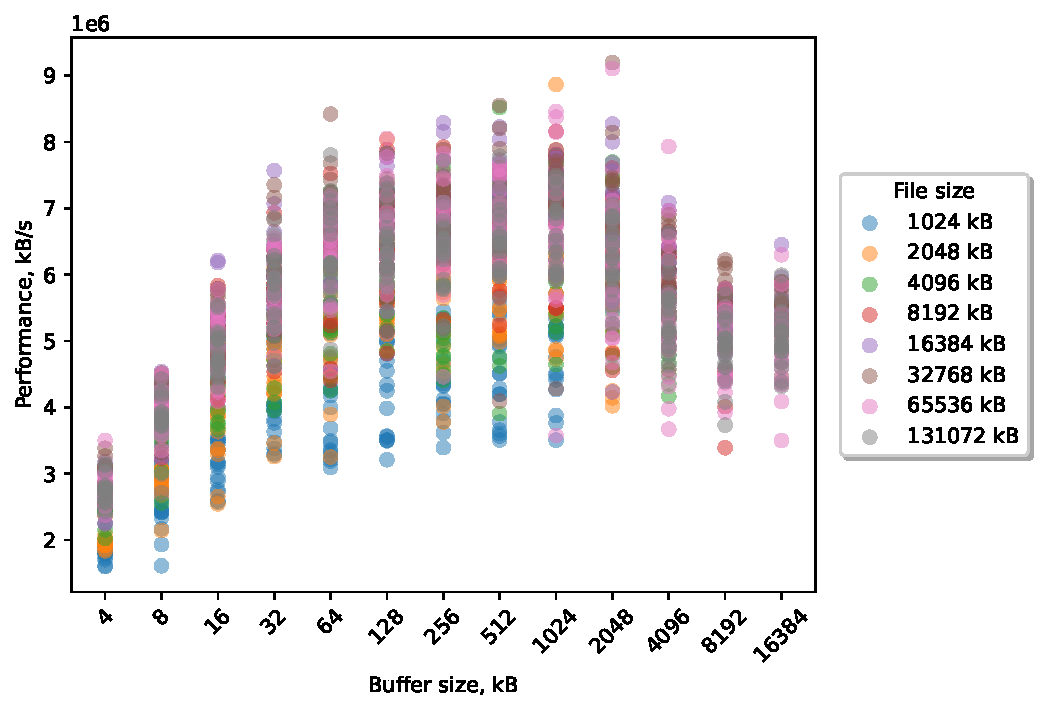
\includegraphics[width=0.8\textwidth]{figures.nosync/benchmarking/GCSF/scatter-UBC Enabled-Re-Read.pdf}
% 	\end{center}
% 	\caption[Comparison of Re-Read performance for file size and buffer size for GCSF with the UBC disabled]{Performance comparison of different file sizes and buffer sizes for GCSF Re-Read with the UBC enabled}
% \end{figure}
% \begin{figure}[!htb]
% 	\label{fig:bench_gcsf_no_ubc_scatter_re-write}
% 	\begin{center}
% 		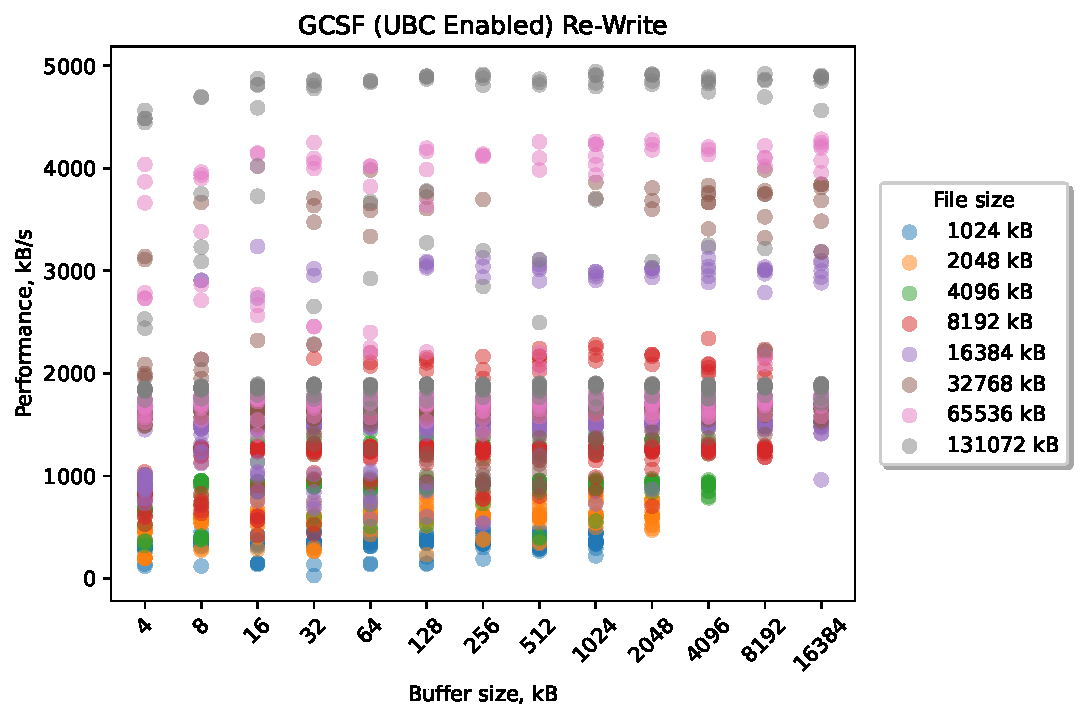
\includegraphics[width=0.8\textwidth]{figures.nosync/benchmarking/GCSF/scatter-UBC Enabled-Re-Write.pdf}
% 	\end{center}
% 	\caption[Comparison of Re-Write performance for file size and buffer size for GCSF with the UBC disabled]{Performance comparison of different file sizes and buffer sizes for GCSF Re-Write with the UBC enabled}
% \end{figure}
% \clearpage
% \begin{figure}[!htb]
% 	\label{fig:bench_gcsf_no_ubc_scatter_rnd_read}
% 	\begin{center}
% 		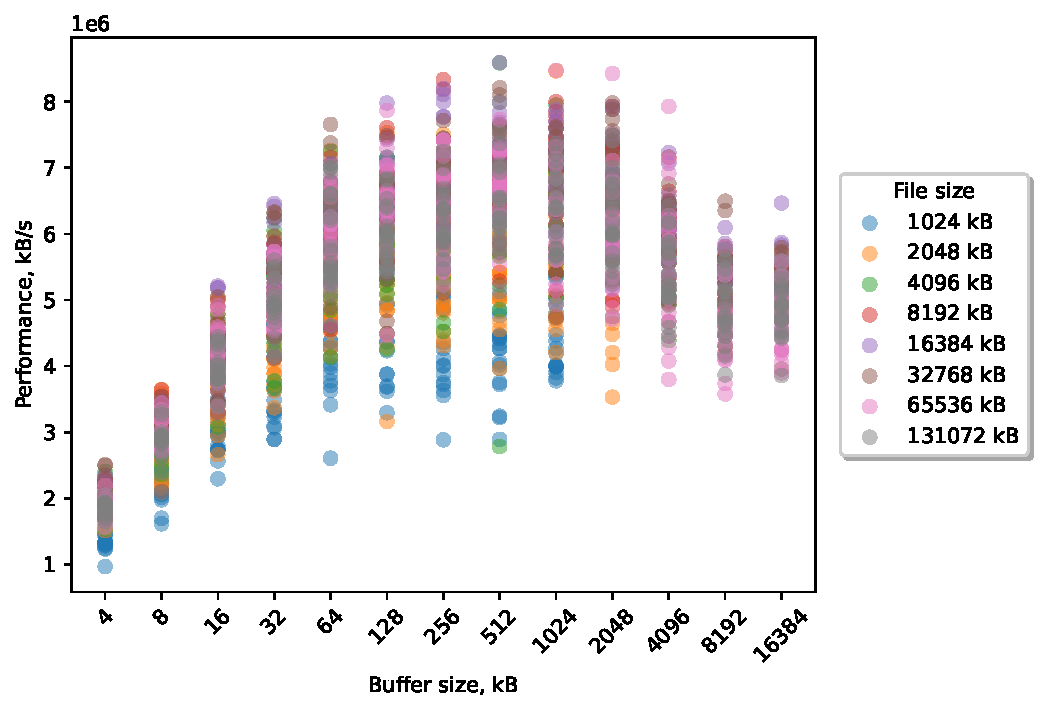
\includegraphics[width=0.8\textwidth]{figures.nosync/benchmarking/GCSF/scatter-UBC Enabled-Random read.pdf}
% 	\end{center}
% 	\caption[Comparison of Random Read performance for file size and buffer size for GCSF with the UBC disabled]{Performance comparison of different file sizes and buffer sizes for GCSF Random Read with the UBC enabled}
% \end{figure}
% \begin{figure}[!htb]
% 	\label{fig:bench_gcsf_no_ubc_scatter_rnd_write}
% 	\begin{center}
% 		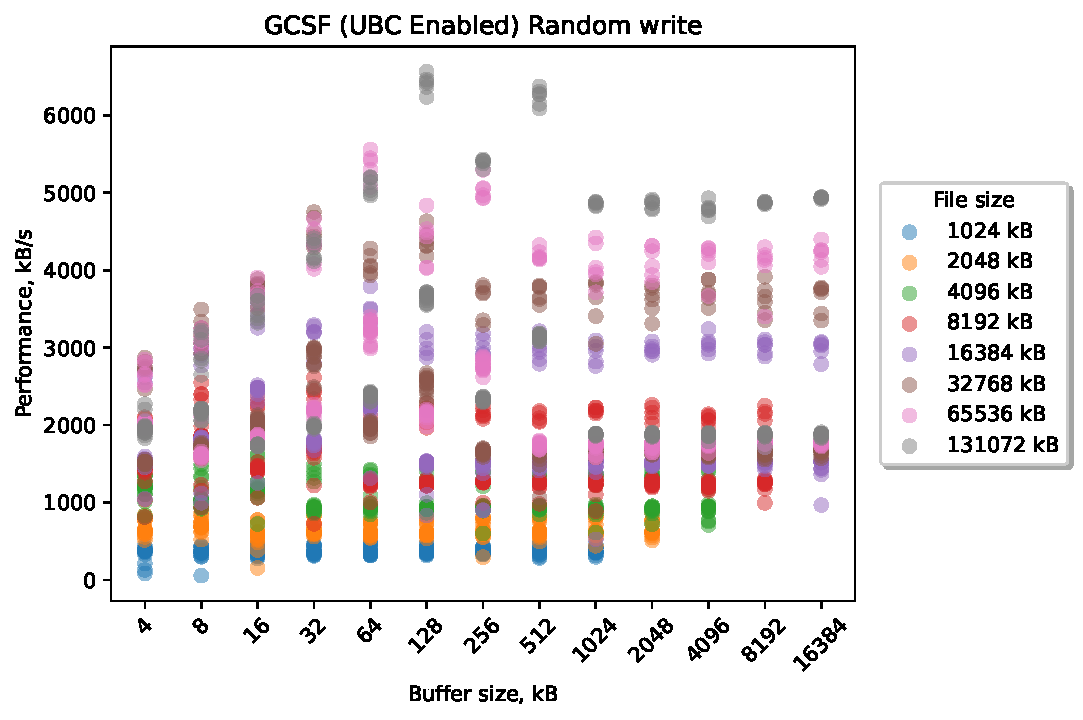
\includegraphics[width=0.8\textwidth]{figures.nosync/benchmarking/GCSF/scatter-UBC Enabled-Random write.pdf}
% 	\end{center}
% 	\caption[Comparison of Random Write performance for file size and buffer size for GCSF with the UBC disabled]{Performance comparison of different file sizes and buffer sizes for GCSF Random Write with the UBC enabled}
% \end{figure}
% \clearpage


% % FFFS

% \begin{figure}[!htb]
% 	\label{fig:bench_fffs_ubc_scatter_read}
% 	\begin{center}
% 		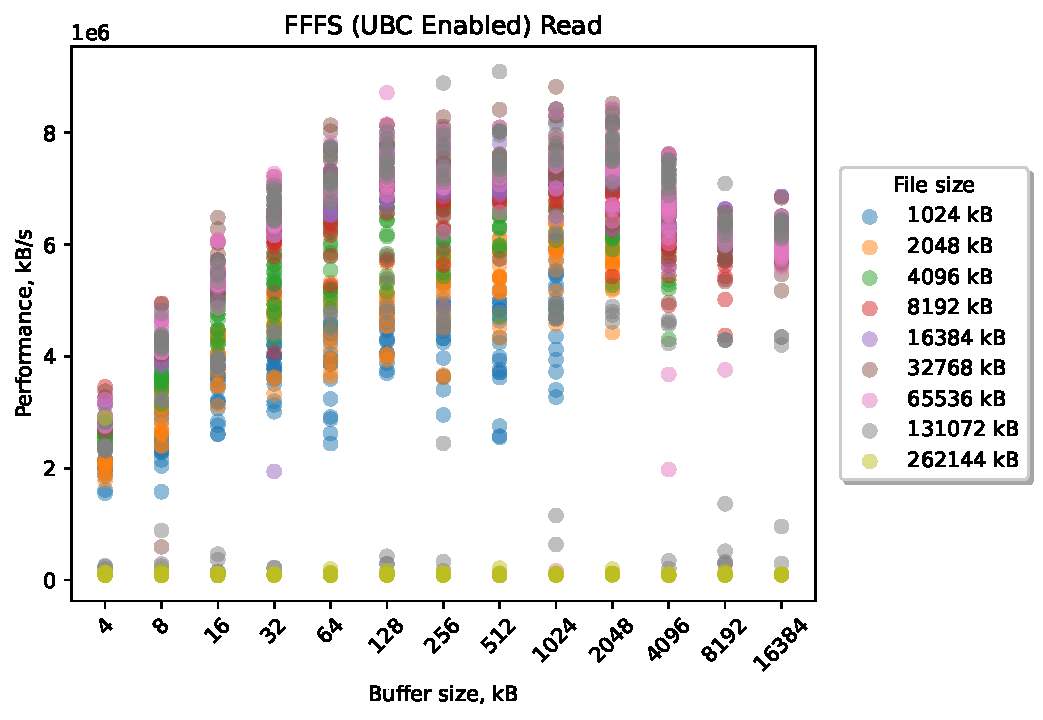
\includegraphics[width=0.8\textwidth]{figures.nosync/benchmarking/FFFS/scatter-UBC Enabled-Read.pdf}
% 	\end{center}
% 	\caption[Comparison of Read performance for file size and buffer size for FFFS with the UBC enabled]{Performance comparison of different file sizes and buffer sizes for FFFS Read with the UBC enabled}
% \end{figure}
% \begin{figure}[!htb]
% 	\label{fig:bench_fffs_ubc_scatter_write}
% 	\begin{center}
% 		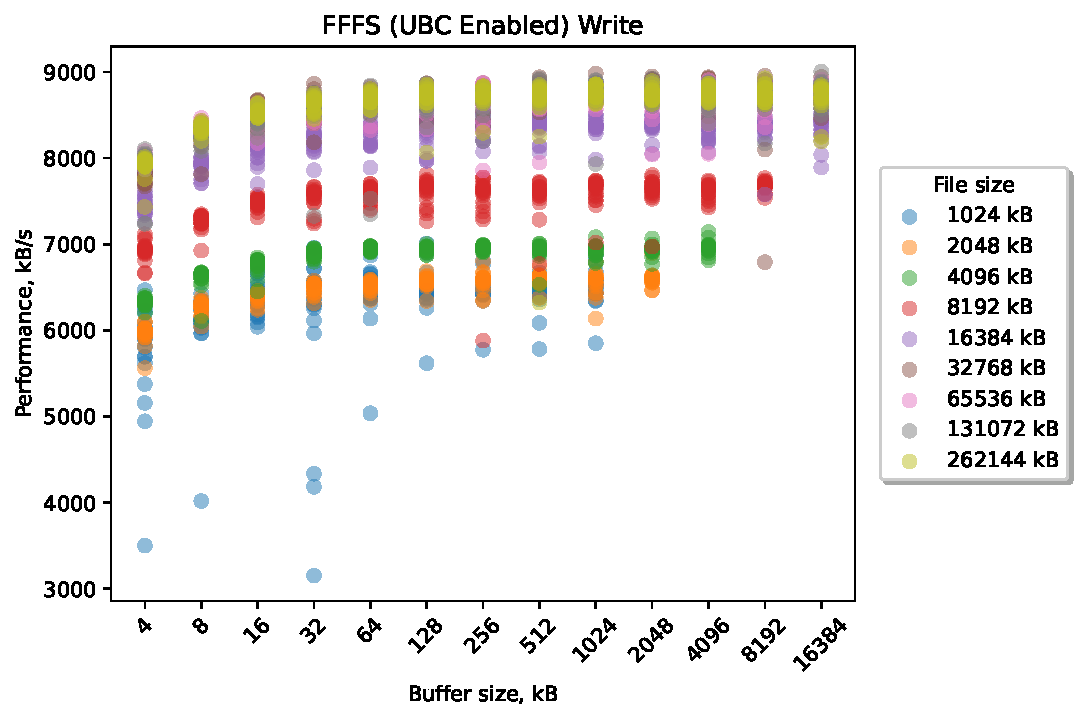
\includegraphics[width=0.8\textwidth]{figures.nosync/benchmarking/FFFS/scatter-UBC Enabled-Write.pdf}
% 	\end{center}
% 	\caption[Comparison of Write performance for file size and buffer size for FFFS with the UBC enabled]{Performance comparison of different file sizes and buffer sizes for FFFS Write with the UBC enabled}
% \end{figure}
% \clearpage
% \begin{figure}[!htb]
% 	\label{fig:bench_fffs_ubc_scatter_re-read}
% 	\begin{center}
% 		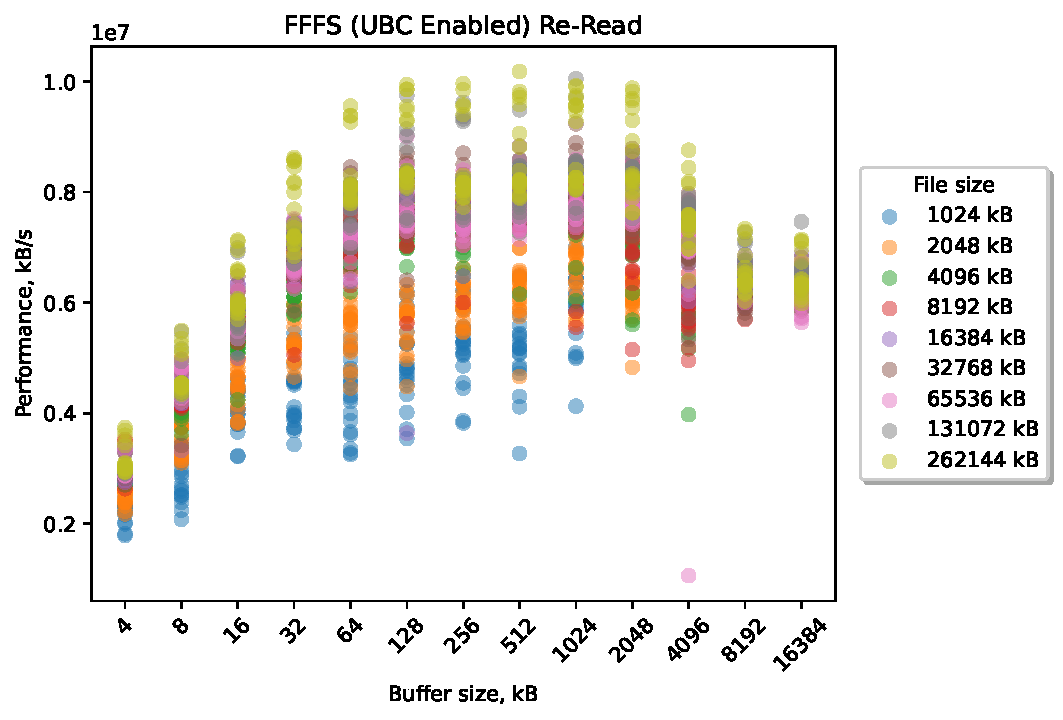
\includegraphics[width=0.8\textwidth]{figures.nosync/benchmarking/FFFS/scatter-UBC Enabled-Re-Read.pdf}
% 	\end{center}
% 	\caption[Comparison of Re-Read performance for file size and buffer size for FFFS with the UBC enabled]{Performance comparison of different file sizes and buffer sizes for FFFS Re-Read with the UBC enabled}
% \end{figure}
% \begin{figure}[!htb]
% 	\label{fig:bench_fffs_ubc_scatter_re-write}
% 	\begin{center}
% 		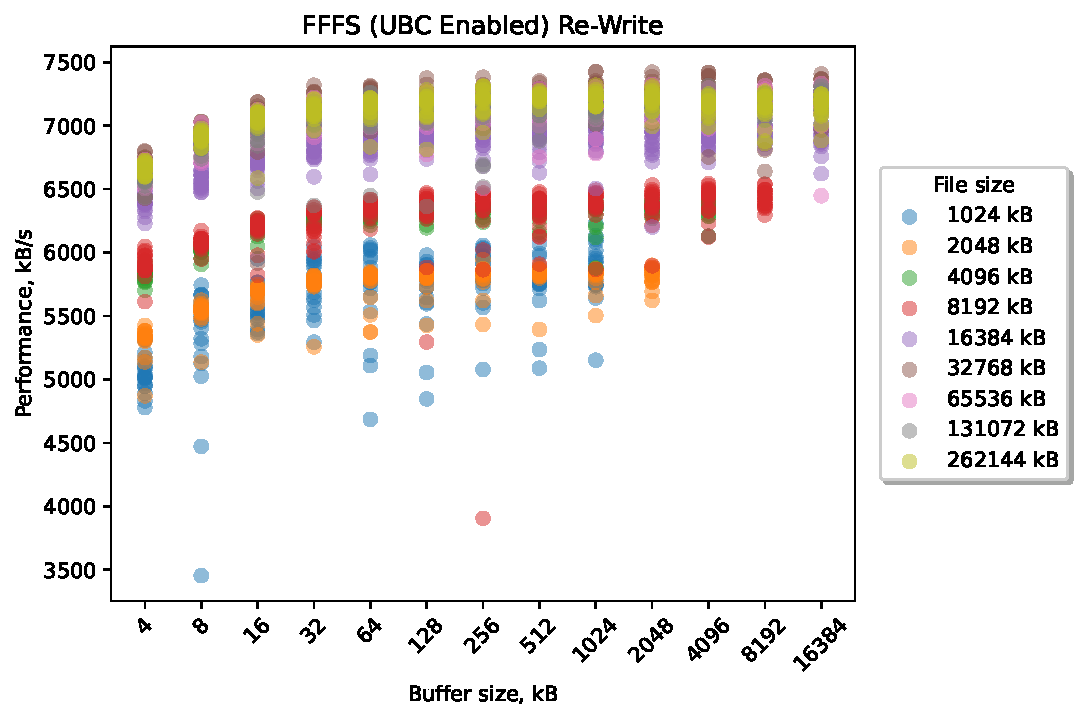
\includegraphics[width=0.8\textwidth]{figures.nosync/benchmarking/FFFS/scatter-UBC Enabled-Re-Write.pdf}
% 	\end{center}
% 	\caption[Comparison of Re-Write performance for file size and buffer size for FFFS with the UBC enabled]{Performance comparison of different file sizes and buffer sizes for FFFS Re-Write with the UBC enabled}
% \end{figure}
% \clearpage
% \begin{figure}[!htb]
% 	\label{fig:bench_fffs_ubc_scatter_rnd_read}
% 	\begin{center}
% 		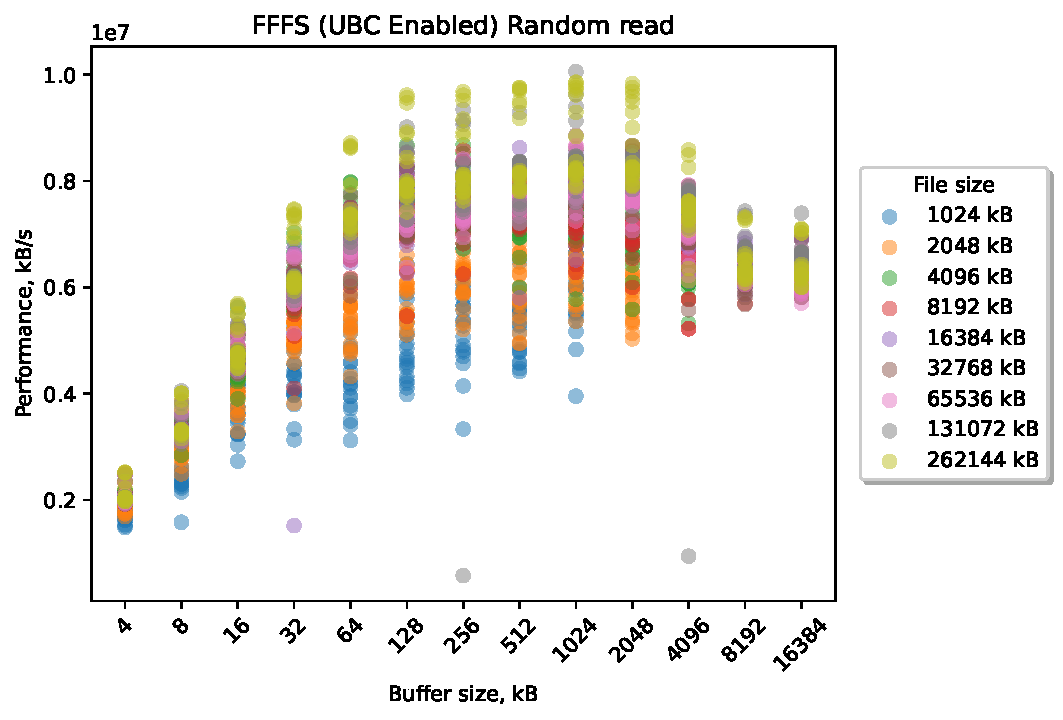
\includegraphics[width=0.8\textwidth]{figures.nosync/benchmarking/FFFS/scatter-UBC Enabled-Random read.pdf}
% 	\end{center}
% 	\caption[Comparison of Random Read performance for file size and buffer size for FFFS with the UBC enabled]{Performance comparison of different file sizes and buffer sizes for FFFS Random Read with the UBC enabled}
% \end{figure}
% \begin{figure}[!htb]
% 	\label{fig:bench_fffs_ubc_scatter_rnd_write}
% 	\begin{center}
% 		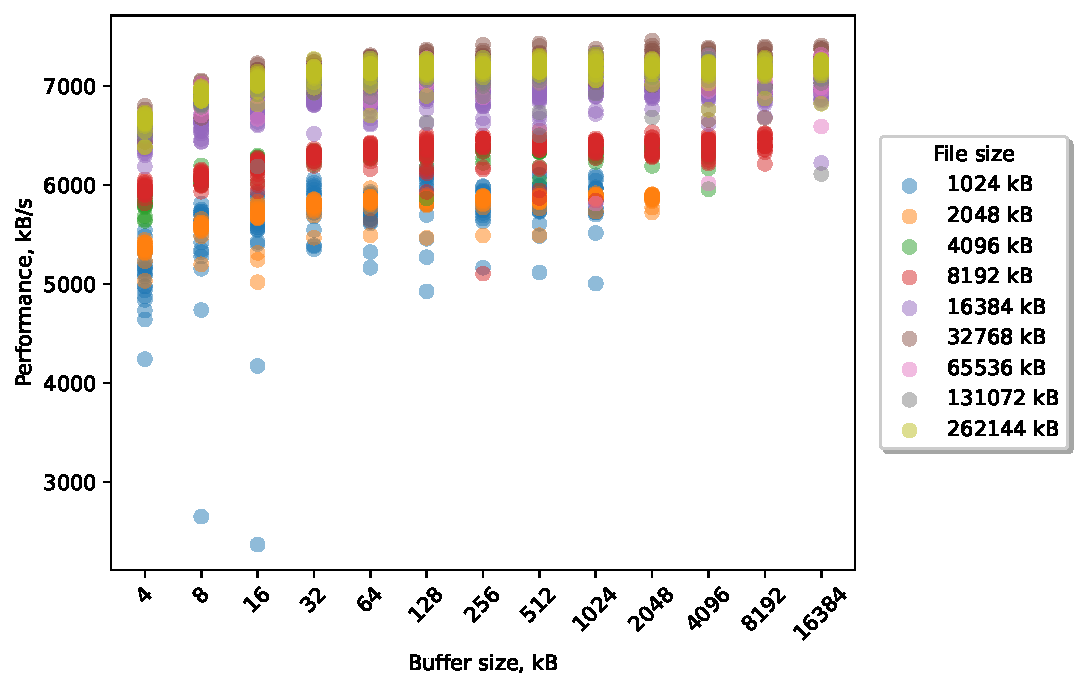
\includegraphics[width=0.8\textwidth]{figures.nosync/benchmarking/FFFS/scatter-UBC Enabled-Random write.pdf}
% 	\end{center}
% 	\caption[Comparison of Random Write performance for file size and buffer size for FFFS with the UBC enabled]{Performance comparison of different file sizes and buffer sizes for FFFS Random Write with the UBC enabled}
% \end{figure}
% \clearpage

% \begin{figure}[!htb]
% 	\label{fig:bench_fffs_no_ubc_scatter_read}
% 	\begin{center}
% 		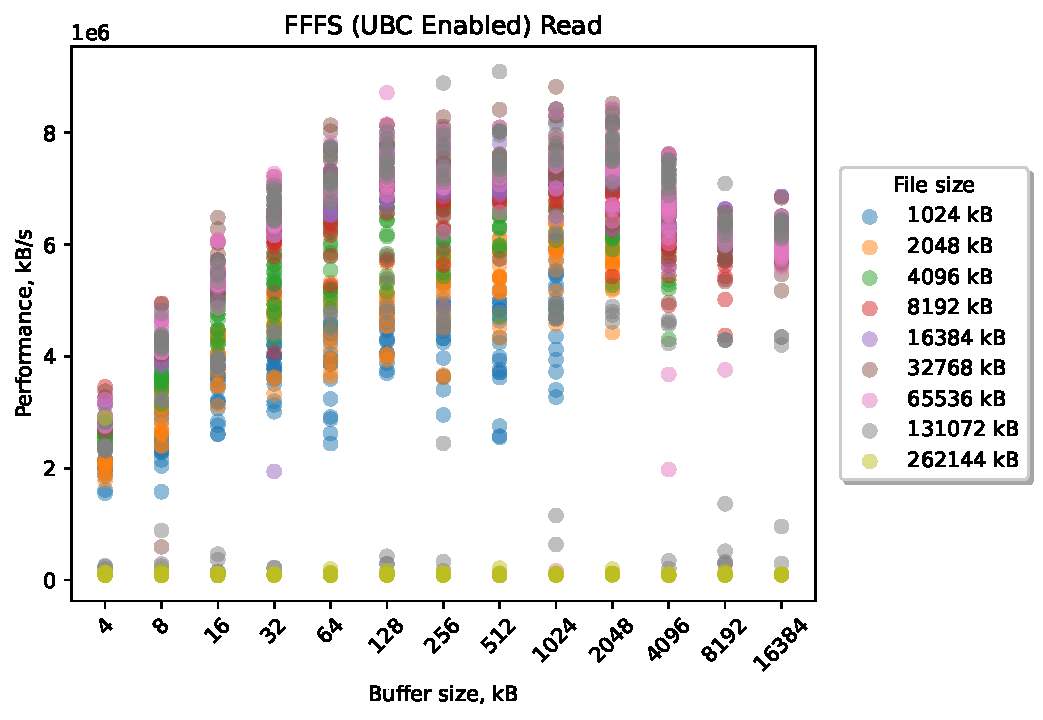
\includegraphics[width=0.8\textwidth]{figures.nosync/benchmarking/FFFS/scatter-UBC Enabled-Read.pdf}
% 	\end{center}
% 	\caption[Comparison of Read performance for file size and buffer size of FFFS with the UBC disabled]{Performance comparison of different file sizes and buffer sizes for FFFS Read with the UBC enabled}
% \end{figure}
% \begin{figure}[!htb]
% 	\label{fig:bench_fffs_no_ubc_scatter_write}
% 	\begin{center}
% 		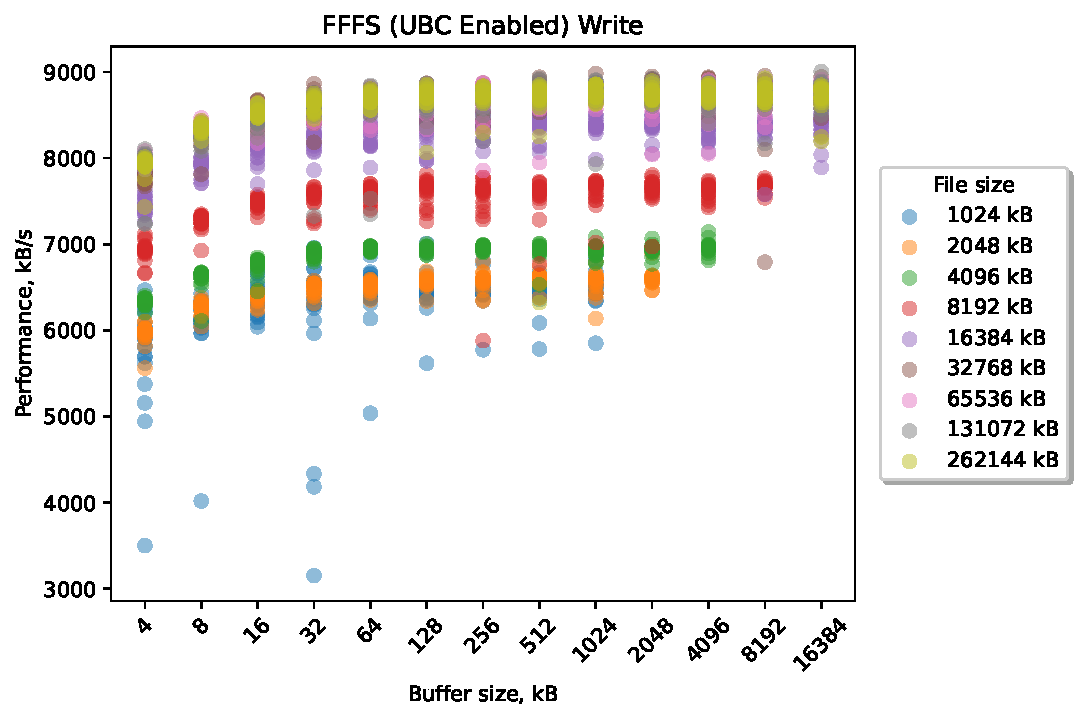
\includegraphics[width=0.8\textwidth]{figures.nosync/benchmarking/FFFS/scatter-UBC Enabled-Write.pdf}
% 	\end{center}
% 	\caption[Comparison of Write performance for file size and buffer size of FFFS with the UBC disabled]{Performance comparison of different file sizes and buffer sizes for FFFS Write with the UBC enabled}
% \end{figure}
% \clearpage
% \begin{figure}[!htb]
% 	\label{fig:bench_fffs_no_ubc_scatter_re-read}
% 	\begin{center}
% 		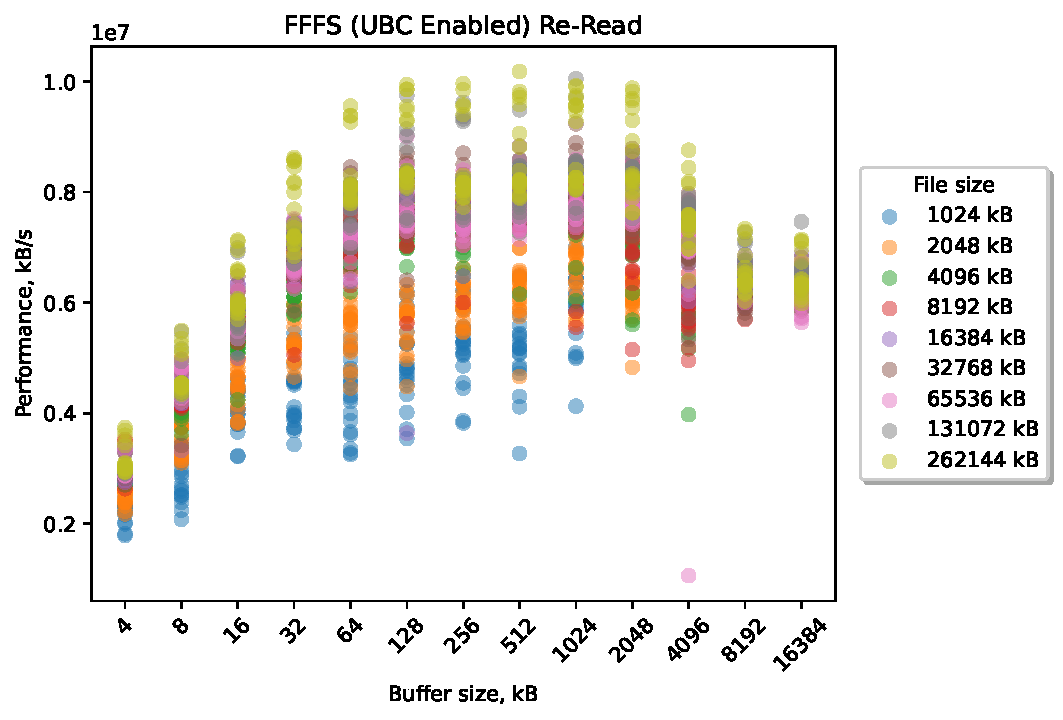
\includegraphics[width=0.8\textwidth]{figures.nosync/benchmarking/FFFS/scatter-UBC Enabled-Re-Read.pdf}
% 	\end{center}
% 	\caption[Comparison of Re-Read performance for file size and buffer size of FFFS with the UBC disabled]{Performance comparison of different file sizes and buffer sizes for FFFS Re-Read with the UBC enabled}
% \end{figure}
% \begin{figure}[!htb]
% 	\label{fig:bench_fffs_no_ubc_scatter_re-write}
% 	\begin{center}
% 		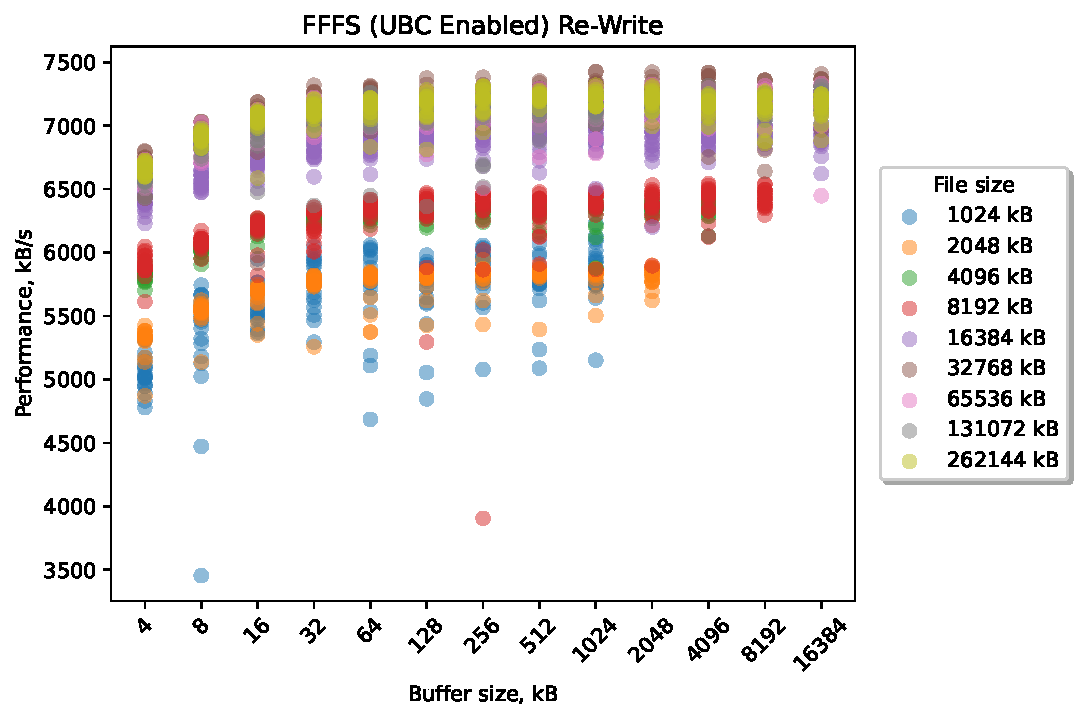
\includegraphics[width=0.8\textwidth]{figures.nosync/benchmarking/FFFS/scatter-UBC Enabled-Re-Write.pdf}
% 	\end{center}
% 	\caption[Comparison of Re-Write performance for file size and buffer size of FFFS with the UBC disabled]{Performance comparison of different file sizes and buffer sizes for FFFS Re-Write with the UBC enabled}
% \end{figure}
% \clearpage
% \begin{figure}[!htb]
% 	\label{fig:bench_fffs_no_ubc_scatter_rnd_read}
% 	\begin{center}
% 		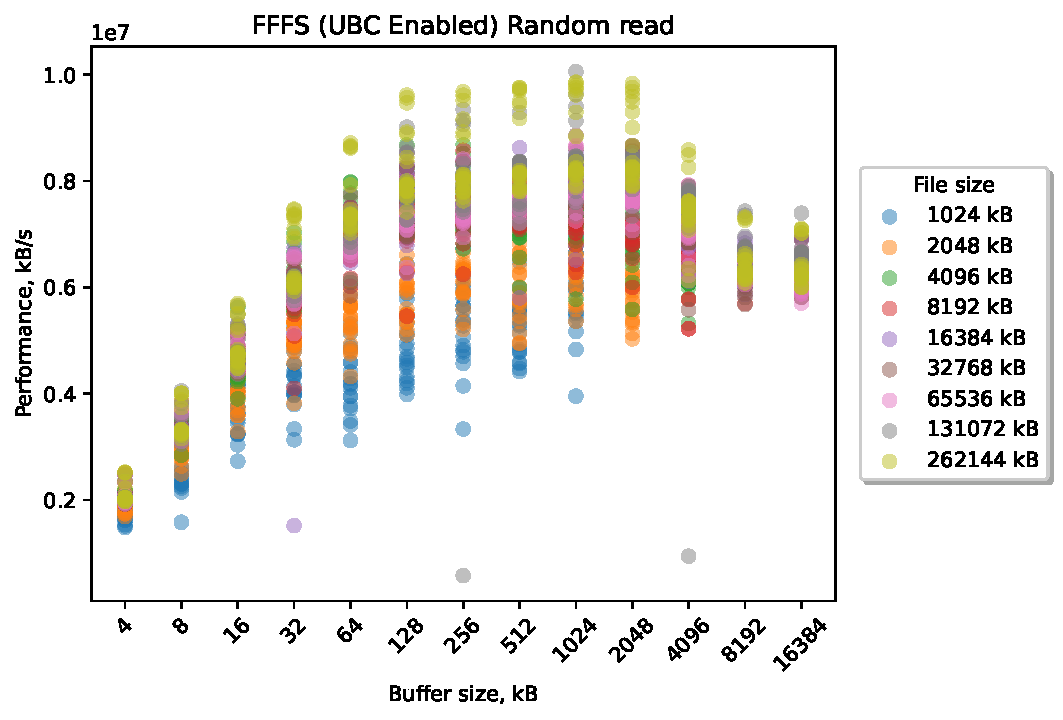
\includegraphics[width=0.8\textwidth]{figures.nosync/benchmarking/FFFS/scatter-UBC Enabled-Random read.pdf}
% 	\end{center}
% 	\caption[Comparison of Random Read performance for file size and buffer size of FFFS with the UBC disabled]{Performance comparison of different file sizes and buffer sizes for FFFS Random Read with the UBC enabled}
% \end{figure}
% \begin{figure}[!htb]
% 	\label{fig:bench_fffs_no_ubc_scatter_rnd_write}
% 	\begin{center}
% 		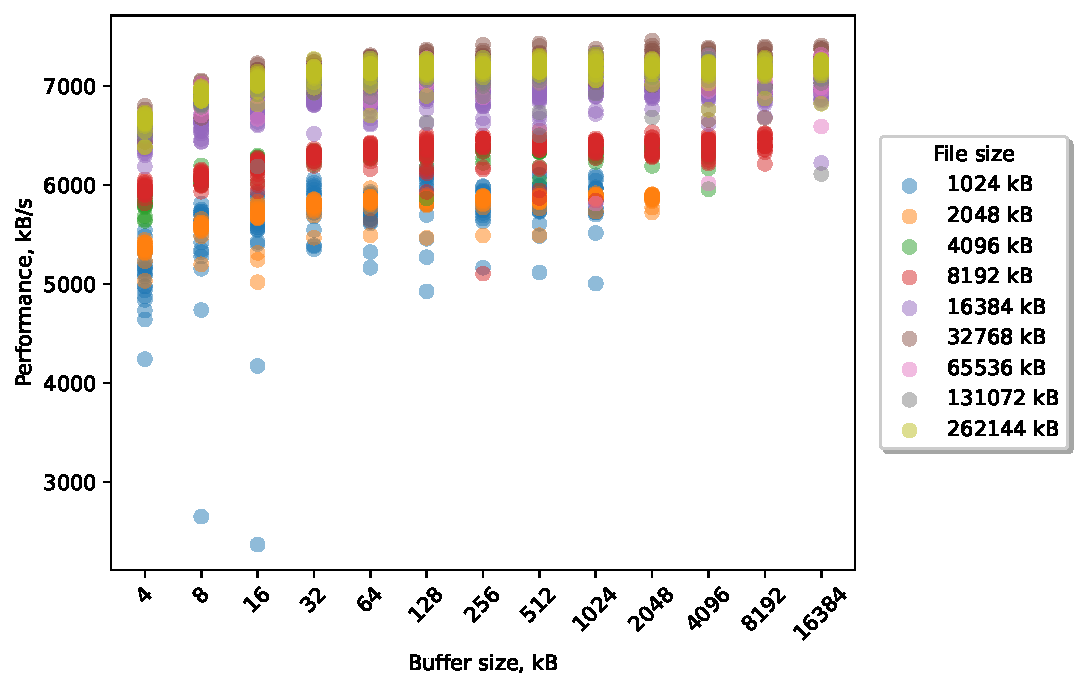
\includegraphics[width=0.8\textwidth]{figures.nosync/benchmarking/FFFS/scatter-UBC Enabled-Random write.pdf}
% 	\end{center}
% 	\caption[Comparison of Random Write performance for file size and buffer size of FFFS with the UBC disabled]{Performance comparison of different file sizes and buffer sizes for FFFS Random Write with the UBC enabled}
% \end{figure}
% \clearpage


% % APFS

% \begin{figure}[!htb]
% 	\label{fig:bench_apfs_ubc_scatter_read}
% 	\begin{center}
% 		\includegraphics[width=0.8\textwidth]{figures.nosync/benchmarking/APFS/scatter-UBC Enabled-Read.pdf}
% 	\end{center}
% 	\caption[Comparison of Read performance for file size and buffer size for APFS with the UBC enabled]{Performance comparison of different file sizes and buffer sizes for APFS Read with the UBC enabled}
% \end{figure}
% \begin{figure}[!htb]
% 	\label{fig:bench_apfs_ubc_scatter_write}
% 	\begin{center}
% 		\includegraphics[width=0.8\textwidth]{figures.nosync/benchmarking/APFS/scatter-UBC Enabled-Write.pdf}
% 	\end{center}
% 	\caption[Comparison of Write performance for file size and buffer size for APFS with the UBC enabled]{Performance comparison of different file sizes and buffer sizes for APFS Write with the UBC enabled}
% \end{figure}
% \clearpage
% \begin{figure}[!htb]
% 	\label{fig:bench_apfs_ubc_scatter_re-read}
% 	\begin{center}
% 		\includegraphics[width=0.8\textwidth]{figures.nosync/benchmarking/APFS/scatter-UBC Enabled-Re-Read.pdf}
% 	\end{center}
% 	\caption[Comparison of Re-Read performance for file size and buffer size for APFS with the UBC enabled]{Performance comparison of different file sizes and buffer sizes for APFS Re-Read with the UBC enabled}
% \end{figure}
% \begin{figure}[!htb]
% 	\label{fig:bench_apfs_ubc_scatter_re-write}
% 	\begin{center}
% 		\includegraphics[width=0.8\textwidth]{figures.nosync/benchmarking/APFS/scatter-UBC Enabled-Re-Write.pdf}
% 	\end{center}
% 	\caption[Comparison of Re-Write performance for file size and buffer size for APFS with the UBC enabled]{Performance comparison of different file sizes and buffer sizes for APFS Re-Write with the UBC enabled}
% \end{figure}
% \clearpage
% \begin{figure}[!htb]
% 	\label{fig:bench_apfs_ubc_scatter_rnd_read}
% 	\begin{center}
% 		\includegraphics[width=0.8\textwidth]{figures.nosync/benchmarking/APFS/scatter-UBC Enabled-Random read.pdf}
% 	\end{center}
% 	\caption[Comparison of Random Read performance for file size and buffer size for APFS with the UBC enabled]{Performance comparison of different file sizes and buffer sizes for APFS Random Read with the UBC enabled}
% \end{figure}
% \begin{figure}[!htb]
% 	\label{fig:bench_apfs_ubc_scatter_rnd_write}
% 	\begin{center}
% 		\includegraphics[width=0.8\textwidth]{figures.nosync/benchmarking/APFS/scatter-UBC Enabled-Random write.pdf}
% 	\end{center}
% 	\caption[Comparison of Random Write performance for file size and buffer size for APFS with the UBC enabled]{Performance comparison of different file sizes and buffer sizes for APFS Random Write with the UBC enabled}
% \end{figure}
% \clearpage

% \begin{figure}[!htb]
% 	\label{fig:bench_apfs_no_ubc_scatter_read}
% 	\begin{center}
% 		\includegraphics[width=0.8\textwidth]{figures.nosync/benchmarking/APFS/scatter-UBC Enabled-Read.pdf}
% 	\end{center}
% 	\caption[Comparison of Read performance for file size and buffer size of APFS with the UBC disabled]{Performance comparison of different file sizes and buffer sizes for APFS Read with the UBC enabled}
% \end{figure}
% \begin{figure}[!htb]
% 	\label{fig:bench_apfs_no_ubc_scatter_write}
% 	\begin{center}
% 		\includegraphics[width=0.8\textwidth]{figures.nosync/benchmarking/APFS/scatter-UBC Enabled-Write.pdf}
% 	\end{center}
% 	\caption[Comparison of Write performance for file size and buffer size of APFS with the UBC disabled]{Performance comparison of different file sizes and buffer sizes for APFS Write with the UBC enabled}
% \end{figure}
% \clearpage
% \begin{figure}[!htb]
% 	\label{fig:bench_apfs_no_ubc_scatter_re-read}
% 	\begin{center}
% 		\includegraphics[width=0.8\textwidth]{figures.nosync/benchmarking/APFS/scatter-UBC Enabled-Re-Read.pdf}
% 	\end{center}
% 	\caption[Comparison of Re-Read performance for file size and buffer size of APFS with the UBC disabled]{Performance comparison of different file sizes and buffer sizes for APFS Re-Read with the UBC enabled}
% \end{figure}
% \begin{figure}[!htb]
% 	\label{fig:bench_apfs_no_ubc_scatter_re-write}
% 	\begin{center}
% 		\includegraphics[width=0.8\textwidth]{figures.nosync/benchmarking/APFS/scatter-UBC Enabled-Re-Write.pdf}
% 	\end{center}
% 	\caption[Comparison of Re-Write performance for file size and buffer size of APFS with the UBC disabled]{Performance comparison of different file sizes and buffer sizes for APFS Re-Write with the UBC enabled}
% \end{figure}
% \clearpage
% \begin{figure}[!htb]
% 	\label{fig:bench_apfs_no_ubc_scatter_rnd_read}
% 	\begin{center}
% 		\includegraphics[width=0.8\textwidth]{figures.nosync/benchmarking/APFS/scatter-UBC Enabled-Random read.pdf}
% 	\end{center}
% 	\caption[Comparison of Random Read performance for file size and buffer size of APFS with the UBC disabled]{Performance comparison of different file sizes and buffer sizes for APFS Random Read with the UBC enabled}
% \end{figure}
% \begin{figure}[!htb]
% 	\label{fig:bench_apfs_no_ubc_scatter_rnd_write}
% 	\begin{center}
% 		\includegraphics[width=0.8\textwidth]{figures.nosync/benchmarking/APFS/scatter-UBC Enabled-Random write.pdf}
% 	\end{center}
% 	\caption[Comparison of Random Write performance for file size and buffer size of APFS with the UBC disabled]{Performance comparison of different file sizes and buffer sizes for APFS Random Write with the UBC enabled}
% \end{figure}
% \clearpage

